
\documentclass[journal,compsoc,10pt]{IEEEtran}
\usepackage[utf8]{inputenc}
\usepackage[T1]{fontenc}
\usepackage{mathptmx} % Times Roman for body + math
\usepackage[scaled=.90]{helvet} % Helvetica for sans-serif
\renewcommand{\sfdefault}{phv}
\DeclareMathAlphabet{\mathsf}{T1}{phv}{m}{n}
\usepackage{courier} % Courier for \texttt monospace
\usepackage{microtype}
\sloppy
\emergencystretch=3em
\hbadness=2000
\vbadness=2000
\hfuzz=2pt
\vfuzz=2pt
\usepackage[hyphens]{url}
\renewcommand{\UrlBreaks}{\do\/\do\-\do\_\do\.\do\:\do\?\do\&\do\=}
\def\BreakableTT#1{\seqsplit{#1}}
\usepackage{cite}
\usepackage{amsmath,amssymb,amsfonts}
\usepackage{amsthm}
\usepackage{mathtools}
\usepackage{algorithmic}
\usepackage{graphicx}
\usepackage{textcomp}
\usepackage{xcolor}
\usepackage{listings}
\usepackage{booktabs}
\usepackage{tabularx}
\usepackage{makecell}
\usepackage{seqsplit}
\usepackage{ragged2e}
\usepackage{enumitem}
\usepackage{hyperref}
\hypersetup{colorlinks=true,linkcolor=black,citecolor=black,urlcolor=black}

\renewcommand{\topfraction}{0.95}
\renewcommand{\bottomfraction}{0.95}
\renewcommand{\textfraction}{0.05}
\renewcommand{\floatpagefraction}{0.7}
\renewcommand{\dbltopfraction}{0.95}
\renewcommand{\dblfloatpagefraction}{0.7}
\setcounter{topnumber}{4}
\setcounter{bottomnumber}{4}
\setcounter{totalnumber}{6}
\setcounter{dbltopnumber}{4}

% --- TikZ (used for the lattice figure) ---
\usepackage{tikz}
\usetikzlibrary{positioning,arrows.meta,calc}

% --- Citation shims: body uses natbib-style \citep/\citet; map to
%     IEEE numeric \cite from the `cite` package. \citet renders as a
%     bare numeric reference under IEEE style. ---
\providecommand{\citep}{\cite}
\providecommand{\citet}{\cite}
\providecommand{\citealp}{\cite}

% --- Listings setup (TLA+ snippet) ---
\lstdefinelanguage{TLA}{
    morekeywords={EXTENDS,VARIABLES,CONSTANTS,ASSUME,THEOREM,DEF,
        TRUE,FALSE,IF,THEN,ELSE,LET,IN,CHOOSE},
    sensitive=true,
    morecomment=[l]{\\*},
}
\lstset{
    basicstyle=\ttfamily\footnotesize,
    columns=fullflexible,
    keepspaces=true,
    frame=single,
    xleftmargin=0pt,
    framesep=3pt,
    breaklines=true
}

% --- Theorem environments ---
\theoremstyle{definition}
\newtheorem{anomaly}{Definition}
\newtheorem{theorem}{Theorem}
% paragraphs are not numbered: a heading printed as 3.1.0.4 Title.: helps nobody
\setcounter{secnumdepth}{3}
\theoremstyle{remark}
\newtheorem*{observation}{Observation}

% --- cleveref (load after hyperref) ---
\usepackage[noabbrev]{cleveref}
\crefname{anomaly}{Definition}{Definitions}
\crefname{paragraph}{Section}{Sections}
\Crefname{paragraph}{Section}{Sections}
\Crefname{anomaly}{Definition}{Definitions}

% ============================================================================
% claims.tex: every headline number, shared with main.tex
% ============================================================================
% claims.tex -- every headline number, as a macro.  Regenerate with
%   python3 harness/macaudit/claims_to_tex.py CLAIMS.json > paper/claims.tex
% so that the paper and CLAIMS.json cannot drift.  VERIFIED-HERE = re-derived
% from committed receipts in this audit; PAPER = carried from the submitted
% artifact's receipts and gated by reproduce.sh but not re-run in this audit.

% --- formal (VERIFIED-HERE unless noted) ---
\newcommand{\VerusCurated}{371}        % PAPER: verus_count.sh under the pinned build 0.2026.09.13 (364 + the 7 of lib_l5_ledger.rs), 2026-10-13
\newcommand{\VerusFull}{392}           % PAPER: verus_count.sh --full under the pinned build
\newcommand{\VerusLoadBearing}{236}    % arithmetic on the per-file table (Sec. 5)
\newcommand{\VerusScaffold}{135}       % arithmetic on the per-file table (+7: the ledger file)
\newcommand{\VerusDetector}{24}        % PAPER
\newcommand{\TlapsHierarchy}{15}       % log committed
\newcommand{\TlapsLowerBound}{28}      % log committed
\newcommand{\TlapsCommitOrder}{60}     % PAPER; tlapm log committed 2026-10-14: formal/tla/tlaps.CommitOrder.log ("All 60 obligations proved")
\newcommand{\CommitOrderVerdicts}{15}  % VERIFIED-HERE
\newcommand{\CommitOrderHistories}{35{,}659}      % VERIFIED-HERE
\newcommand{\CommitOrderMemoryStates}{2{,}961{,}434} % VERIFIED-HERE
\newcommand{\LatticeRuns}{64}          % VERIFIED-HERE (6-run sample identical to reference; full matrix in reference json)
\newcommand{\LatticeMaxOpsThreeRuns}{16}
\newcommand{\LatticeSafeStatesMin}{380{,}920}
\newcommand{\LatticeSafeStatesMax}{2{,}015{,}279}

% --- live LangGraph A1 study (VERIFIED-HERE, incl. the outcome columns) ---
\newcommand{\LiveNPerCell}{100}
\newcommand{\LiveGptVanillaAOne}{60}
\newcommand{\LiveHaikuVanillaAOne}{91}
\newcommand{\LiveLlamaVanillaAOne}{1}
\newcommand{\LiveGptValidatedWrong}{34}
\newcommand{\LiveHaikuValidatedWrong}{7}
\newcommand{\LiveLlamaValidatedWrong}{100}
\newcommand{\LiveGptRegen}{66}
\newcommand{\LiveHaikuRegen}{93}
\newcommand{\LiveGptPinnedMean}{1.07}
\newcommand{\LiveGptPinnedMax}{3.79}
\newcommand{\LiveHaikuPinnedMean}{1.21}
\newcommand{\LiveHaikuPinnedMax}{1.96}
\newcommand{\LiveLlamaPinnedMean}{3.77}
\newcommand{\LiveLlamaPinnedMax}{9.06}
\newcommand{\LiveOffsetMs}{150}
\newcommand{\SuperstepGpt}{42}
\newcommand{\SuperstepHaiku}{72}
\newcommand{\SuperstepLlama}{26}

% --- AutoGen pilot (VERIFIED-HERE via rescore) ---
\newcommand{\PilotTriageRates}{42\%, 48\% and 52\%}
\newcommand{\PilotTriagePooled}{142/300}
\newcommand{\PilotSiEditResidual}{5}
\newcommand{\PilotSiTriageResidual}{8}

% --- cost (VERIFIED-HERE: workcost.py, realstore_metrics.py --check) ---
\newcommand{\CostRun}{20260913T0150Z}

% --- L2 / L4 / A6 (PAPER; receipts to be committed as results/*.json) ---
\newcommand{\LtwoDefThreeBaseline}{519, 624 and 563}
\newcommand{\LtwoExposedBaseline}{1{,}538, 2{,}059 and 2{,}010}
\newcommand{\LtwoExposedVerified}{402, 547 and 549}
\newcommand{\LtwoRelabeled}{767, 1{,}288 and 1{,}239}
\newcommand{\LiveLtwoRetractions}{66}
\newcommand{\LfourPhantom}{630, 505 and 387}

% --- ToolNode A6 (VERIFIED-HERE from per-turn receipts) ---
\newcommand{\ToolNodeGptBatched}{30}
\newcommand{\ToolNodeGptReordered}{22}
\newcommand{\ToolNodeGptFull}{18}
\newcommand{\ToolNodeLlamaBatched}{3}
\newcommand{\ToolNodeLlamaReordered}{2}
\newcommand{\ToolNodeBatchedTurns}{33}
\newcommand{\ToolNodeReorderings}{24}

% --- census (VERIFIED-HERE: langgraph_census.py --summary/--check) ---
\newcommand{\CensusRepos}{98}
\newcommand{\CensusSites}{407}
\newcommand{\CensusSequential}{392}
\newcommand{\CensusParallelRepos}{11}
\newcommand{\CensusUpperRepos}{8}
\newcommand{\CensusErrorStringRepos}{34}

% --- residue predicate R (artifact: A7 / NoA7) and the ledger (added 2026-10-13) ---
% VERIFIED-HERE: A7 witness (3 s), NoA7 exhaustive under G7 (5,213,012 states; 9,688,601 with G3), the full lattice32 matrix (160 runs, 0 mismatches),
% the partition A1+A7 = booking!=final on every live cell (harness/macaudit/a7_rescore.py --check).
\newcommand{\AsevenGptVanilla}{40}
\newcommand{\AsevenHaikuVanilla}{9}
\newcommand{\AsevenLlamaVanilla}{99}
\newcommand{\AsevenGptValidated}{34}
\newcommand{\AsevenHaikuValidated}{7}
\newcommand{\AsevenLlamaValidated}{100}
\newcommand{\LatticeThirtyTwoRuns}{160}
\newcommand{\LatticeThirtyTwoSafeMin}{1{,}803{,}848}   % VERIFIED-HERE (lattice32_results.reference.json)
\newcommand{\LatticeThirtyTwoSafeMax}{9{,}688{,}601}
\newcommand{\NoAsevenStates}{5{,}213{,}012}
\newcommand{\NoAsevenStatesGthree}{9{,}688{,}601}
% PENDING (your machine): verus count for lib_l5_ledger.rs; probe 303 --modes ledger outcome
\newcommand{\LfiveVerus}{7 obligations, 0 errors}   % results/verus/lib_l5_ledger.verus.log, pinned build
% short forms for the abstract / intro: replace with "verified, N obligations" once lib_l5_ledger.rs verifies
\newcommand{\LfiveVerusStatus}{verified in Verus (7 obligations, 0 errors)}
\newcommand{\LfiveVerusIntro}{verified (7 obligations)}
\newcommand{\LfiveLiveOutcome}{\textbf{[probe 303 -{}-modes ledger: pending]}}
% per-cell defaults for the verified / ledger rows of Table 3 ("--" = pending); claims_results.tex overrides
\newcommand{\Pend}{--}
\newcommand{\LiveVerifiedGptAOne}{\Pend}\newcommand{\LiveVerifiedGptR}{\Pend}\newcommand{\LiveVerifiedGptWrong}{\Pend}\newcommand{\LiveVerifiedGptRegen}{\Pend}
\newcommand{\LiveVerifiedHaikuAOne}{\Pend}\newcommand{\LiveVerifiedHaikuR}{\Pend}\newcommand{\LiveVerifiedHaikuWrong}{\Pend}\newcommand{\LiveVerifiedHaikuRegen}{\Pend}
\newcommand{\LiveLedgerGptAOne}{\Pend}\newcommand{\LiveLedgerGptR}{\Pend}\newcommand{\LiveLedgerGptWrong}{\Pend}\newcommand{\LiveLedgerGptRegen}{\Pend}
\newcommand{\LiveLedgerHaikuAOne}{\Pend}\newcommand{\LiveLedgerHaikuR}{\Pend}\newcommand{\LiveLedgerHaikuWrong}{\Pend}\newcommand{\LiveLedgerHaikuRegen}{\Pend}
\newcommand{\LiveVerifiedLlamaAOne}{\Pend}\newcommand{\LiveVerifiedLlamaR}{\Pend}\newcommand{\LiveVerifiedLlamaWrong}{\Pend}\newcommand{\LiveVerifiedLlamaRegen}{\Pend}
\newcommand{\LiveLedgerLlamaAOne}{\Pend}\newcommand{\LiveLedgerLlamaR}{\Pend}\newcommand{\LiveLedgerLlamaWrong}{\Pend}\newcommand{\LiveLedgerLlamaRegen}{\Pend}
% probe 301 / 302 defaults
\newcommand{\ToolNodeRealSqlite}{\textbf{[probe 301: pending]}}
\newcommand{\ToolNodeRealHttp}{\textbf{[probe 301: pending]}}
\newcommand{\WallclockPairedGptAvailable}{0}\newcommand{\WallclockPairedClaudeAvailable}{0}
\newcommand{\WallclockPairedGptTriagePess}{\Pend}\newcommand{\WallclockPairedGptTriageSI}{\Pend}
\newcommand{\WallclockPairedGptEditReviewPess}{\Pend}\newcommand{\WallclockPairedGptEditReviewSI}{\Pend}
\newcommand{\WallclockPairedGptPlanExecutePess}{\Pend}\newcommand{\WallclockPairedGptPlanExecuteSI}{\Pend}
\newcommand{\WallclockPairedClaudeTriagePess}{\Pend}\newcommand{\WallclockPairedClaudeTriageSI}{\Pend}
\newcommand{\WallclockPairedClaudeEditReviewPess}{\Pend}\newcommand{\WallclockPairedClaudeEditReviewSI}{\Pend}
\newcommand{\WallclockPairedClaudePlanExecutePess}{\Pend}\newcommand{\WallclockPairedClaudePlanExecuteSI}{\Pend}
\newcommand{\OffsetCurveAvailable}{0}
\newcommand{\LatticeThirtyTwoOutcome}{All \LatticeThirtyTwoRuns{} runs match their expectation (0 mismatches); the exhaustive runs range over 1{,}803{,}848--9{,}688{,}601 distinct states, and the sixty-four commit-time cells with $G_7$ off return the verdicts of \texttt{lattice16.sh} one for one.}
\newcommand{\LiveVerifiedOutcome}{\textbf{[probe 303 -{}-modes verified: pending]}}

% --- hypothesis gates (VERIFIED-HERE: harness/macaudit/hypothesis_gates.py --tex, over every committed record) ---
\newcommand{\HypRecords}{36{,}036}     % hypothesis_gates.py over results/ on 2026-10-14: 25,637 September + 9,649 probe 303 + 750 Claude op-record pilot
\newcommand{\HypTraces}{10{,}488}      % 6,588 + 3,600 + 300
\newcommand{\HypSameAgentOverlaps}{0}
\newcommand{\HypReadBeforeCommitViolations}{0}
\newcommand{\HypCampaigns}{16}
\newcommand{\HypValueUniqueCampaigns}{10}
\newcommand{\HypCollisionCells}{126}
\newcommand{\HypCollisionTraces}{105}
\newcommand{\HypLiveLtwoSessions}{600}
\newcommand{\HypLiveLtwoCollisions}{0}
\newcommand{\HypAOneWitnesses}{710}    % 292 + 418
\newcommand{\HypRestored}{0}
\newcommand{\HypBookings}{4{,}500}      % 900 + 3,600
\newcommand{\HypBasisRecovered}{4{,}500}
% two-value safety half of lattice16 on the CURRENT model (lattice16_v2.sh); filled in by finalize
\newcommand{\LatticeVtwoOutcome}{all $32$ safety runs \textsc{safe}, $2.4$--$17.3$M states}
\newcommand{\LiveLtwoHaikuThousand}{\Pend}

% a fourth API family (DeepSeek, OpenAI-compatible endpoint) -- all four arms "--" until step 2 runs
\newcommand{\LiveVanillaDeepseekAOne}{\Pend}\newcommand{\LiveVanillaDeepseekR}{\Pend}\newcommand{\LiveVanillaDeepseekWrong}{\Pend}\newcommand{\LiveVanillaDeepseekRegen}{\Pend}
\newcommand{\LiveValidatedDeepseekAOne}{\Pend}\newcommand{\LiveValidatedDeepseekR}{\Pend}\newcommand{\LiveValidatedDeepseekWrong}{\Pend}\newcommand{\LiveValidatedDeepseekRegen}{\Pend}
\newcommand{\LiveVerifiedDeepseekAOne}{\Pend}\newcommand{\LiveVerifiedDeepseekR}{\Pend}\newcommand{\LiveVerifiedDeepseekWrong}{\Pend}\newcommand{\LiveVerifiedDeepseekRegen}{\Pend}
\newcommand{\LiveLedgerDeepseekAOne}{\Pend}\newcommand{\LiveLedgerDeepseekR}{\Pend}\newcommand{\LiveLedgerDeepseekWrong}{\Pend}\newcommand{\LiveLedgerDeepseekRegen}{\Pend}
\newcommand{\LiveVanillaSonnetAOne}{\Pend}\newcommand{\LiveVanillaSonnetR}{\Pend}\newcommand{\LiveVanillaSonnetWrong}{\Pend}\newcommand{\LiveVanillaSonnetRegen}{\Pend}
\newcommand{\LiveValidatedSonnetAOne}{\Pend}\newcommand{\LiveValidatedSonnetR}{\Pend}\newcommand{\LiveValidatedSonnetWrong}{\Pend}\newcommand{\LiveValidatedSonnetRegen}{\Pend}
\newcommand{\LiveVerifiedSonnetAOne}{\Pend}\newcommand{\LiveVerifiedSonnetR}{\Pend}\newcommand{\LiveVerifiedSonnetWrong}{\Pend}\newcommand{\LiveVerifiedSonnetRegen}{\Pend}
\newcommand{\LiveLedgerSonnetAOne}{\Pend}\newcommand{\LiveLedgerSonnetR}{\Pend}\newcommand{\LiveLedgerSonnetWrong}{\Pend}\newcommand{\LiveLedgerSonnetRegen}{\Pend}

% ============================================================================
% claims_results.tex (2026-10-14): the receipt overrides generated by harness/macaudit/claims_from_results.py
% ============================================================================
% generated by harness/macaudit/claims_from_results.py -- do not edit; re-run the probes instead
% --- probe 303 (results/live_a1_outcome; *_arms150.json -> Table 3, *_sweep.json -> offset curve) ---
\renewcommand{\LiveVanillaDeepseekAOne}{$45/100$ [35.0, 55.3]}
\renewcommand{\LiveVanillaDeepseekR}{$55$}
\renewcommand{\LiveVanillaDeepseekWrong}{$100/100$ [96.4, 100.0]}
\renewcommand{\LiveVanillaDeepseekRegen}{0}
\renewcommand{\LiveValidatedDeepseekAOne}{$0/100$ [0.0, 3.6]}
\renewcommand{\LiveValidatedDeepseekR}{$63$}
\renewcommand{\LiveValidatedDeepseekWrong}{$63/100$ [52.8, 72.4]}
\renewcommand{\LiveValidatedDeepseekRegen}{37}
\renewcommand{\LiveVerifiedGptAOne}{$0/100$ [0.0, 3.6]}
\renewcommand{\LiveVerifiedGptR}{$51$}
\renewcommand{\LiveVerifiedGptWrong}{$51/100$ [40.8, 61.1]}
\renewcommand{\LiveVerifiedGptRegen}{49}
\renewcommand{\LiveLedgerGptAOne}{$0/100$ [0.0, 3.6]}
\renewcommand{\LiveLedgerGptR}{$0$}
\renewcommand{\LiveLedgerGptWrong}{$0/100$ [0.0, 3.6]}
\renewcommand{\LiveLedgerGptRegen}{55$+$45 (45/45 obl.)}
\renewcommand{\LiveVerifiedHaikuAOne}{$0/100$ [0.0, 3.6]}
\renewcommand{\LiveVerifiedHaikuR}{$2$}
\renewcommand{\LiveVerifiedHaikuWrong}{$2/100$ [0.2, 7.0]}
\renewcommand{\LiveVerifiedHaikuRegen}{98}
\renewcommand{\LiveLedgerHaikuAOne}{$0/100$ [0.0, 3.6]}
\renewcommand{\LiveLedgerHaikuR}{$0$}
\renewcommand{\LiveLedgerHaikuWrong}{$0/100$ [0.0, 3.6]}
\renewcommand{\LiveLedgerHaikuRegen}{95$+$5 (5/5 obl.)}
\renewcommand{\LiveVerifiedDeepseekAOne}{$0/100$ [0.0, 3.6]}
\renewcommand{\LiveVerifiedDeepseekR}{$52$}
\renewcommand{\LiveVerifiedDeepseekWrong}{$52/100$ [41.8, 62.1]}
\renewcommand{\LiveVerifiedDeepseekRegen}{48}
\renewcommand{\LiveLedgerDeepseekAOne}{$0/100$ [0.0, 3.6]}
\renewcommand{\LiveLedgerDeepseekR}{$0$}
\renewcommand{\LiveLedgerDeepseekWrong}{$0/100$ [0.0, 3.6]}
\renewcommand{\LiveLedgerDeepseekRegen}{47$+$53 (53/53 obl.)}
\renewcommand{\LiveVerifiedOutcome}{$A_1=0/300$; booking $\neq$ final $2$, $51$, $52$ of $100$ on haiku, gpt-4o-mini, deepseek-chat}
\renewcommand{\LfiveLiveOutcome}{booking $\neq$ final $0/100$ on all three families (5, 45, 53 obligations, all discharged)}
\providecommand{\SweepHaikuVanillaOZ}{46/5/51}
\providecommand{\SweepHaikuVanillaOOXZ}{47/4/51}
\providecommand{\SweepHaikuVanillaOXZZ}{4/40/44}
\providecommand{\SweepHaikuVanillaOOXZZ}{0/44/44}
\providecommand{\SweepHaikuValidatedOZ}{0/2/2}
\providecommand{\SweepHaikuValidatedOOXZ}{0/4/4}
\providecommand{\SweepHaikuValidatedOXZZ}{0/46/46}
\providecommand{\SweepHaikuValidatedOOXZZ}{0/42/42}
\providecommand{\SweepGptVanillaOZ}{40/11/51}
\providecommand{\SweepGptVanillaOOXZ}{36/15/51}
\providecommand{\SweepGptVanillaOXZZ}{1/43/44}
\providecommand{\SweepGptVanillaOOXZZ}{0/44/44}
\providecommand{\SweepGptValidatedOZ}{0/4/4}
\providecommand{\SweepGptValidatedOOXZ}{0/13/13}
\providecommand{\SweepGptValidatedOXZZ}{0/40/40}
\providecommand{\SweepGptValidatedOOXZZ}{0/42/42}
\providecommand{\SweepDeepseekVanillaOZ}{39/12/51}
\providecommand{\SweepDeepseekVanillaOOXZ}{20/31/51}
\providecommand{\SweepDeepseekVanillaOXZZ}{2/42/44}
\providecommand{\SweepDeepseekVanillaOOXZZ}{0/44/44}
\providecommand{\SweepDeepseekValidatedOZ}{0/17/17}
\providecommand{\SweepDeepseekValidatedOOXZ}{0/26/26}
\providecommand{\SweepDeepseekValidatedOXZZ}{0/52/52}
\providecommand{\SweepDeepseekValidatedOOXZZ}{0/42/42}
\renewcommand{\OffsetCurveAvailable}{1}
% --- verus ledger (results/verus/lib_l5_ledger.verus.log) ---
\renewcommand{\LfiveVerus}{7 obligations, 0 errors}
\renewcommand{\LfiveVerusStatus}{verified in Verus (7 obligations, 0 errors)}
\renewcommand{\LfiveVerusIntro}{verified (7 obligations)}
% --- merged from b4fca224-paper_receipts_summary.json (receipts absent in this checkout) ---
\renewcommand{\ToolNodeRealSqlite}{$126/165$}
\renewcommand{\ToolNodeRealHttp}{$112/165$}
% a regenerated claims_results.tex beside this file (run_experiments.sh step 13) overrides the block above
\IfFileExists{claims_results.tex}{% generated by harness/macaudit/claims_from_results.py -- do not edit; re-run the probes instead
% --- probe 303 (results/live_a1_outcome; *_arms150.json -> Table 3, *_sweep.json -> offset curve) ---
\renewcommand{\LiveVanillaDeepseekAOne}{$45/100$ [35.0, 55.3]}
\renewcommand{\LiveVanillaDeepseekR}{$55$}
\renewcommand{\LiveVanillaDeepseekWrong}{$100/100$ [96.4, 100.0]}
\renewcommand{\LiveVanillaDeepseekRegen}{0}
\renewcommand{\LiveValidatedDeepseekAOne}{$0/100$ [0.0, 3.6]}
\renewcommand{\LiveValidatedDeepseekR}{$63$}
\renewcommand{\LiveValidatedDeepseekWrong}{$63/100$ [52.8, 72.4]}
\renewcommand{\LiveValidatedDeepseekRegen}{37}
\renewcommand{\LiveVerifiedGptAOne}{$0/100$ [0.0, 3.6]}
\renewcommand{\LiveVerifiedGptR}{$51$}
\renewcommand{\LiveVerifiedGptWrong}{$51/100$ [40.8, 61.1]}
\renewcommand{\LiveVerifiedGptRegen}{49}
\renewcommand{\LiveLedgerGptAOne}{$0/100$ [0.0, 3.6]}
\renewcommand{\LiveLedgerGptR}{$0$}
\renewcommand{\LiveLedgerGptWrong}{$0/100$ [0.0, 3.6]}
\renewcommand{\LiveLedgerGptRegen}{55$+$45 (45/45 obl.)}
\renewcommand{\LiveVerifiedHaikuAOne}{$0/100$ [0.0, 3.6]}
\renewcommand{\LiveVerifiedHaikuR}{$2$}
\renewcommand{\LiveVerifiedHaikuWrong}{$2/100$ [0.2, 7.0]}
\renewcommand{\LiveVerifiedHaikuRegen}{98}
\renewcommand{\LiveLedgerHaikuAOne}{$0/100$ [0.0, 3.6]}
\renewcommand{\LiveLedgerHaikuR}{$0$}
\renewcommand{\LiveLedgerHaikuWrong}{$0/100$ [0.0, 3.6]}
\renewcommand{\LiveLedgerHaikuRegen}{95$+$5 (5/5 obl.)}
\renewcommand{\LiveVerifiedDeepseekAOne}{$0/100$ [0.0, 3.6]}
\renewcommand{\LiveVerifiedDeepseekR}{$52$}
\renewcommand{\LiveVerifiedDeepseekWrong}{$52/100$ [41.8, 62.1]}
\renewcommand{\LiveVerifiedDeepseekRegen}{48}
\renewcommand{\LiveLedgerDeepseekAOne}{$0/100$ [0.0, 3.6]}
\renewcommand{\LiveLedgerDeepseekR}{$0$}
\renewcommand{\LiveLedgerDeepseekWrong}{$0/100$ [0.0, 3.6]}
\renewcommand{\LiveLedgerDeepseekRegen}{47$+$53 (53/53 obl.)}
\renewcommand{\LiveVerifiedOutcome}{$A_1=0/300$; booking $\neq$ final $2$, $51$, $52$ of $100$ on haiku, gpt-4o-mini, deepseek-chat}
\renewcommand{\LfiveLiveOutcome}{booking $\neq$ final $0/100$ on all three families (5, 45, 53 obligations, all discharged)}
\providecommand{\SweepHaikuVanillaOZ}{46/5/51}
\providecommand{\SweepHaikuVanillaOOXZ}{47/4/51}
\providecommand{\SweepHaikuVanillaOXZZ}{4/40/44}
\providecommand{\SweepHaikuVanillaOOXZZ}{0/44/44}
\providecommand{\SweepHaikuValidatedOZ}{0/2/2}
\providecommand{\SweepHaikuValidatedOOXZ}{0/4/4}
\providecommand{\SweepHaikuValidatedOXZZ}{0/46/46}
\providecommand{\SweepHaikuValidatedOOXZZ}{0/42/42}
\providecommand{\SweepGptVanillaOZ}{40/11/51}
\providecommand{\SweepGptVanillaOOXZ}{36/15/51}
\providecommand{\SweepGptVanillaOXZZ}{1/43/44}
\providecommand{\SweepGptVanillaOOXZZ}{0/44/44}
\providecommand{\SweepGptValidatedOZ}{0/4/4}
\providecommand{\SweepGptValidatedOOXZ}{0/13/13}
\providecommand{\SweepGptValidatedOXZZ}{0/40/40}
\providecommand{\SweepGptValidatedOOXZZ}{0/42/42}
\providecommand{\SweepDeepseekVanillaOZ}{39/12/51}
\providecommand{\SweepDeepseekVanillaOOXZ}{20/31/51}
\providecommand{\SweepDeepseekVanillaOXZZ}{2/42/44}
\providecommand{\SweepDeepseekVanillaOOXZZ}{0/44/44}
\providecommand{\SweepDeepseekValidatedOZ}{0/17/17}
\providecommand{\SweepDeepseekValidatedOOXZ}{0/26/26}
\providecommand{\SweepDeepseekValidatedOXZZ}{0/52/52}
\providecommand{\SweepDeepseekValidatedOOXZZ}{0/42/42}
\renewcommand{\OffsetCurveAvailable}{1}
% --- probe 301 (results/a6_real_latency/sqlite.jsonl) ---
\renewcommand{\ToolNodeRealSqlite}{$126/165$}
% --- probe 301 (results/a6_real_latency/http.jsonl) ---
\renewcommand{\ToolNodeRealHttp}{$112/165$}
% --- probe 302 (results/runs/20261014T0617Z-interleaved; model gpt-4o) ---
\renewcommand{\WallclockPairedGptAvailable}{1}
% --- verus ledger (results/verus/lib_l5_ledger.verus.log) ---
\renewcommand{\LfiveVerus}{7 obligations, 0 errors}
\renewcommand{\LfiveVerusStatus}{verified in Verus (7 obligations, 0 errors)}
\renewcommand{\LfiveVerusIntro}{verified (7 obligations)}
}{}

\providecommand{\A}[1]{$A_{#1}$}
% --- Field-name macros ---
\newcommand{\fld}[1]{\mathit{#1}}
\newcommand{\rs}{\fld{read\_set}}
\newcommand{\ws}{\fld{write\_set}}
\newcommand{\rt}{\fld{read\_time}}
\newcommand{\wt}{\fld{write\_time}}
\newcommand{\rv}{\fld{read\_values}}
\newcommand{\wv}{\fld{write\_values}}
\newcommand{\rreg}{\fld{read\_registry}}
\newcommand{\wreg}{\fld{write\_registry}}
\newcommand{\pt}{\fld{planned\_tool}}

% --- Float packing: reduce float-page whitespace (typesetting only) ---
\renewcommand{\topfraction}{0.92}
\renewcommand{\bottomfraction}{0.85}
\renewcommand{\textfraction}{0.06}
\renewcommand{\floatpagefraction}{0.80}
\renewcommand{\dbltopfraction}{0.92}
\renewcommand{\dblfloatpagefraction}{0.80}
\setcounter{topnumber}{3}
\setcounter{bottomnumber}{2}
\setcounter{totalnumber}{5}
\setcounter{dbltopnumber}{3}

\usepackage{array}
\providecommand{\TLA}{TLA\textsuperscript{+}}
\begin{document}
\renewcommand{\thetable}{S\arabic{table}}
\renewcommand{\thefigure}{S\arabic{figure}}

\title{Online Appendix to:\\ Verified Detection and Prevention of Concurrency
Anomalies in Multi-Agent Large Language Model Systems}
\author{Sajjad Khan}
\markboth{Supplementary Material}{}
\maketitle

\IEEEraisesectionheading{\section*{}}

\noindent This supplement collects the raw experimental and benchmarking tables
referenced from the main paper (Tables S1--S6) and the material moved out of
it for length. Each table is referenced by
its S-number from the main text; the surrounding analysis, findings, and
interpretation remain in the main paper. Appendices~G--S hold material moved out of the main paper for length; it is the main paper's own text, with its cross-references rewritten to point into the main paper or into this appendix. The full reproducibility artifact
accompanies this appendix: \texttt{verus\_count.sh} regenerates the obligation
totals against the working tree, and \texttt{check\_tables.sh} rescores every
published cell of the main paper's Tables~3, 4 and 7 with an implementation of
Definition~1 independent of the Verus-verified detector, failing non-zero on any
disagreement.


\section*{Appendix A: Concurrent-semantics lift --- full development}

The four refinement proofs of the main paper hold under sequential interleaving:
agent operations occur one at a time, atomically. This appendix develops the
lift from sequential to concurrent semantics under an \emph{abstract} mutex
protocol.

\medskip
\noindent\textbf{What this lift now covers, and what it does not.} Since the two
guarded stores were rebuilt on \texttt{vstd}'s verified reader--writer lock, the
deployed snapshot-isolation and pessimistic-locking stores assume nothing about
a lock: their safety is established directly, on every state reachable under the
verified lock, and \texttt{parking\_lot::Mutex} is gone from both. The lift
below therefore \emph{does not describe a deployed guarded runtime}. It remains
the mechanized statement of what an abstract lock must satisfy for the
sequential refinement proofs to apply to a multi-threaded execution, and it is
retained for that purpose. What still locks with \texttt{parking\_lot::Mutex} is
the agent client's pending-operation cell and the unguarded vanilla store, which
is the $L_0$ baseline and carries no safety claim.

\medskip
\noindent\textbf{Atomic-event model.} We define a concurrent operational
semantics in which each runtime step is an atomic event of one of four kinds:
\texttt{LockAcquire(a,c,t)}, \texttt{LockRelease(a,c,t)}, \texttt{Read(a,c,t,v)}
and \texttt{Write(a,c,t,v)}, where $a$ is the agent, $c$ the cell, $t$ a
monotonic timestamp and $v$ a value. A concurrent trace is a sequence of such
events. The runtime state at any prefix is a $\langle$holders, values$\rangle$
pair: a map from cells to currently-holding agents (absent keys mean unlocked)
and a map from cells to current values.

A step function \texttt{step(s,e)} transitions the state: \texttt{LockAcquire}
adds $(c \mapsto a)$ to holders, \texttt{LockRelease} removes $c$,
\texttt{Read} leaves $s$ unchanged, \texttt{Write} updates
\texttt{values[c] := v}. The companion enabling predicate
\texttt{step\_enabled(s,e)} encodes the abstract mutex protocol:
\texttt{LockAcquire} requires the cell to be unlocked; \texttt{LockRelease} and
accesses require the acting agent to currently hold the cell's lock; a
\texttt{Read} must observe the cell's current value if one exists. A trace
$\tau$ is well-formed iff every event in $\tau$ is enabled from its preceding
state.

\medskip
\noindent\textbf{Verified theorems.} The development
(\texttt{lib\_concurrent\_semantics.rs}; 9 verified, 0 errors, 0 axioms)
establishes: prefix monotonicity; mutex exclusion (at most one holder per cell);
access implies lock held; reads observe the current value (no torn reads);
distinct-agent access separation; and a helper that a holder change requires an
intervening lock event.

\medskip
\noindent\textbf{Lift to sequential refinement.} Distinct-agent access
separation is the key result: per cell, the access events in a well-formed
concurrent trace project to a strictly serialized sequence. The per-cell
projection is exactly the sequential trace shape consumed by the refinement
proofs, so any well-formed concurrent trace is observationally equivalent (per
cell) to a sequential trace.

\medskip
\noindent\textbf{Scope, and the structural-tautology caveat.} This lift has a
structural-tautology character: well-formedness encodes the abstract protocol as
a precondition on events, and the safety consequences follow from that encoding.
It is not a verification of any concrete runtime; it is an identification, in
mechanically-verified form, of the precise abstract protocol the sequential
refinement proofs require.

\medskip
\noindent\textbf{Bounded weak-memory validation.} While the abstract lift
assumes sequential consistency, we additionally check the lock protocol under
the RC11 weak-memory model~\cite{lahav2017} with the GenMC stateless model
checker~\cite{genmc2021}. Encoding the acquire--read--generate--write--release
discipline as $N$ concurrent locked read--modify--writes on a shared cell,
GenMC exhaustively reports no lost update---a lost update being exactly an $A_1$
witness---for $N \in \{2,3,4\}$ (2, 6 and 24 complete executions). A
relaxed-ordering control, with the acquire-CAS and release-store weakened to
\texttt{memory\_order\_relaxed}, is reported as a data race with a concrete
counterexample, confirming the release/acquire ordering is load-bearing. This
does not extend to unbounded $N$, nor does it verify that any particular mutex
implements the protocol.

\section*{Appendix B: RustBelt interface specification --- full obligations}

\noindent\textbf{What this is and is not.} The file
\texttt{verus-detector/src/lib\_rustbelt\_interface.rs} is not a RustBelt proof.
RustBelt~\cite{rustbelt2018} is a verified type system for Rust built on Iris;
producing a RustBelt-grade verification of a mutex requires working inside Iris.
What the file is: an explicit, mechanized specification of the obligations such a
verification would discharge.

\medskip
\noindent\textbf{These obligations describe no deployed guarded runtime.} Both
guarded stores now run on \texttt{vstd}'s own verified reader--writer lock, so
none of the obligations below is on the path of a deployed safety claim. They
are retained as the statement of what the abstract lift of Appendix~A requires
of a lock.

\medskip
\noindent\textbf{The four obligations.}
\begin{enumerate}
\item \texttt{lock\_is\_acquire}: acquiring the lock corresponds to the abstract
      \texttt{LockAcquire} event.
\item \texttt{drop\_is\_release}: dropping the guard corresponds to
      \texttt{LockRelease}; the borrow checker ensures the guard cannot outlive
      the critical section.
\item \texttt{event\_seqcst}: the Rust memory model plus the LLVM pipeline
      preserve the total order of Acquire/Release events the event-level model
      assumes.
\item \texttt{no\_panic\_in\_critical\_section}: a property of the runtime
      source, not of any mutex. Unlike 1--3 this is not a bare stub: the same
      file proves 4a, panic-freedom of the modeled critical sections, and 4b,
      fail-safety under lock poisoning.
\end{enumerate}

\noindent Obligation 4b is moreover no longer needed by the guarded stores: both
install state only through the verified lock's release path, which requires the
invariant, so a panic inside a critical section cannot leave a torn store. The
residual stub count is therefore three, matching the trust-base accounting of
the main paper. This appendix does not close the concurrency gap; it makes the
residual auditable as three named obligations rather than a collective
assumption.

\section*{Appendix C: MAST --- topological susceptibility and dynamic
confirmation}

\noindent\textbf{Structural susceptibility across canonical topologies.} The
necessary condition for cross-agent $A_1$ has a purely structural part---two
agents scheduled in one superstep where one reads a state channel the other
writes---decidable from a graph's layers and per-node read/write channels alone,
independent of any model output. This is
\texttt{lib\_l2\_safety.rs::a1\_witness} with the value inequality existentially
relaxed, hence a sound over-approximation: a topology found non-susceptible
cannot exhibit cross-agent $A_1$ at runtime for any input or model.

We applied it to sixteen canonical, publicly documented topologies---LangGraph
supervisor fan-out, map-reduce with and without a reducer, orchestrator-workers,
parallel tool calls, routing, reflection, evaluator-optimizer, plan-and-execute,
hierarchical teams, collaboration, swarm, a memory chatbot, CrewAI sequential
staging, multi-agent debate and the classic blackboard architecture---plus two
controls. Six of sixteen are structurally susceptible: hierarchical teams,
collaboration, swarm, blackboard, competing-agents consensus and a reducer-less
map-reduce, in every case because concurrent agents read and write one shared
mutable channel within a superstep. The other ten are immune by construction:
disjoint result channels, an additive reducer, or strictly sequential staging.
The contrast is sharpest between the reducer-based map-reduce (immune) and an
identical workload with a read-modify-written shared accumulator (susceptible),
isolating the reducer---not the workload---as the safety mechanism. The positive
control is flagged and the negative control is not. The analyzer
(\texttt{prevalence\_static.py}) is deterministic and dependency-free.

\medskip
\noindent\textbf{The precision this bound requires, and what a framework
supplies.}
\label{sec:extraction-precision}
The read and write channel sets above are declared, not recovered, and the
distinction they support is fragile in a specific and measurable way.
\texttt{python/langgraph\_extract.py} builds the same four topologies as real
LangGraph graphs, scores the same structural predicate over a $2 \times 2$
matrix of declared and extracted read and write sets, and reports:

\begin{center}
\begin{tabular}{lc}
\toprule
read set / write set & susceptible \\
\midrule
declared / declared \quad (the encoding above) & 1 of 4 \\
declared / extracted & 3 of 4 \\
extracted / declared & 3 of 4 \\
extracted / extracted \quad (a real front end) & 3 of 4 \\
\bottomrule
\end{tabular}
\end{center}

Losing precision on either side collapses the split, so both are
load-bearing---but the two sides are not alike. The read set is
over-approximated by default, because a compiled node reports the whole state
schema, and it is \emph{recoverable}: annotating a node with
\texttt{add\_node(\ldots, input\_schema=S)} narrows what the framework reports
to that node's declared channels. The write set is not recoverable at any
annotation effort: LangGraph 1.2 has no per-node output schema and its
\texttt{ChannelWrite} carries \texttt{static=None}, because the channels a node
writes are whatever dictionary its body returns at run time. The obvious escape
does not work either: the reducer flag
(\texttt{BinaryOperatorAggregate} versus \texttt{LastValue}) is the one
discriminating fact the compiled object does expose, but a last-value rule
built on it reproduces the $1$-of-$4$ split only when write sets are already
known, and returns $3$ of $4$ otherwise---it needs the same missing input.

\medskip
\noindent\textbf{A shape the runtime refuses.} Running the same graphs rather
than only reading them adds one more constraint, and it cuts across the
encoding. LangGraph rejects two co-superstep nodes writing one
non-reducer channel at execution time: \texttt{LastValue.update} raises
\texttt{InvalidUpdateError}, ``At key `$c$': Can receive only one value per
step.'' Of the four graphs above, three execute and the one the encoding calls
susceptible does not. Every one of the six susceptible topologies in
\texttt{prevalence\_static.py} has two or more co-layer writers on the cell it
is flagged for---\texttt{shared\_scratch}, \texttt{messages},
\texttt{active\_agent}, \texttt{blackboard}, \texttt{proposals},
\texttt{accumulator}---so for those of them intended as LangGraph graphs, the
flagged shape is one the runtime will not run without a reducer, and a reducer
is what the encoding calls immune.

This does not make $A_1$ vacuous in LangGraph, and the distinction matters. A
reader sharing a channel with a \emph{single} co-superstep writer is
susceptible and does execute; that is the deployable shape, and it is the one
the main paper's live cross-agent stale-generation study measures. The
structural bound and the live measurement are therefore about different
shapes, and we say so rather than let the two zeros and the $k$-of-$N$ figure
be read as one body of evidence.

\medskip
\noindent\textbf{What an instrumented run recovers.} The write set is the one
input static extraction cannot supply, and it is precisely what a single
instrumented execution observes, because a node's update dictionary
\emph{is} its write set. \texttt{prevalence\_harness.instrument\_layered}
wraps every node of a graph, derives each node's superstep from the graph's
own edges, and records an operation per node; on the three runnable graphs
above the observed write sets matched the declared ones exactly. That is why
the corpus instrument (\texttt{python/prevalence\_corpus.py}) wraps nodes
rather than reading the compiled object, and it is the method a third-party
corpus study would use.

We therefore state the bound's scope rather than leave it to be discovered.
The $k$-of-$N$ figure characterizes \emph{documented architectures under a
declared encoding}. Turning it into a design-time analysis over third-party
graphs requires one framework affordance that does not exist today and that is
symmetric with one that does: a per-node write declaration to match the
per-node \texttt{input\_schema}. That is a concrete request to framework
authors, and it is the gating item for the static robustness procedure the main
paper's future-work section describes, rather than an engineering detail of
it.

\medskip
\noindent\textbf{Dynamic confirmation, and exactly what it confirms.} Each
susceptible topology is instantiated in its unconditionally-concurrent form in a
small BSP/superstep executor in which each node is a real model call
(\texttt{prevalence\_dynamic\_run.py}), and all nine instantiations were run for
$n = 20$ trials on each of the two model families whose $360$ session records
the artifact carries: \texttt{gpt-4o-mini} and \texttt{claude-haiku-4-5}. The
outcome is identical on both: every structurally-immune topology and the
negative control fired in $0/20$, while every susceptible instantiation and the
positive control fired in $20/20$ (exact 95\,\% Clopper--Pearson
$[0.83, 1.00]$). Scored with the \emph{superstep} form of the predicate---a
co-superstep write of a different value by another agent---since each round is a
single superstep whose commits land at one tick.

Two limits of that run are load-bearing and we state them rather than let the
$20/20$ carry more than it can. First, the superstep form is a \emph{different}
relaxation of Definition~1 from the structural predicate above: the structural
analyzer drops the value conjunct and keeps the ordering, while the executor
keeps the value conjunct and drops the window. Because the executor stamps each
record's read and commit as consecutive ticks, all $1{,}320$ committed records
have window width one, and rescoring the same records under the full
Definition~1 yields $0/360$---the identical width-one limitation the
cookbook-derived and MAST-Data tables below declare for their own corpora. Second, the executor
pre-populates every cell with a sentinel so that first-layer reads are recorded
at all, and all $520$ superstep firings are reads of that sentinel; none is an
agent reading a value another agent produced. Both facts are recomputable from
the committed records in \texttt{python/dynamic\_oprecords}.

What the run therefore establishes is that a superstep executor does schedule
the structurally susceptible topologies concurrently on a shared channel, and
the immune ones not---the structural precondition exercised rather than
inferred. It is not an independent measurement of value-conflicting $A_1$, and
the main paper does not use it as one. This demarcates the \emph{structural}
scope of $A_1$ rather than estimating prevalence: absent by construction from
reducer- and fan-out-structured deployments, structurally present in
shared-mutable-cell designs run concurrently. The value-conflicting measurement
is the live study of the main paper's Section~6.1, where the window is real.

\medskip
\noindent\textbf{Superseded as a prevalence instrument.} The main paper's Section~6.8 replaces this bound with a static census of public repositories, which recovers per-node write sets from source rather than asking the framework for them: $407$ graph sites in $98$ sampled repositories, none with a confirmed co-scheduled reader and writer of a last-value channel.

\section*{Appendix D: Locating contemporary runtimes on the chain --- full
placements}

Offered as illustrative discussion, not a formal contribution. Each placement is
approximate, based on published descriptions rather than source analysis, and
conditional on workload assumptions made explicit per runtime. We report each
runtime's avoidance set as a subset of $\{A_1,A_2,A_3,A_6\}$, naming a chain
level only when the set is on-chain.

\medskip
\noindent\textbf{SagaLLM~\cite{sagallm}: avoidance set $\{A_3\}$ (off-chain) on
compensable workloads.} Saga-style compensation addresses $A_3$ by retracting
external effects when their basis is invalidated (conditional on reversibility).
It does not address $A_1$ (no read-set tracking), $A_2$ (no registry stability)
or $A_6$ (no intra-operation write atomicity). The set is $\{A_3\}$ on
compensable workloads, $\emptyset$ ($L_0$) where effects are irreversible, and
$\{A_1,A_3\}$ ($L_2$) with a complementary OCC layer.

\medskip
\noindent\textbf{Atomix~\cite{atomix}: avoidance set varies by workload.} Atomix
tags tool calls with epochs, tracks per-resource frontiers and commits only when
progress predicates indicate safety; the frontier-gated commit prevents
intra-operation reordering ($\neg A_6$) and compensation handles retraction
($\neg A_3$, modulo irreversibility). $A_1$ prevention depends on whether
read-sets are frontier-tracked: yes for explicit dependencies, no for implicit.
The set is $\{A_1,A_3,A_6\}$ ($L_3$, on-chain) on explicit-dependency
compensable workloads, and $\{A_3,A_6\}$ or $\{A_6\}$ (off-chain) otherwise.

\medskip
\noindent\textbf{CodeCRDT~\cite{codecrdt}: avoidance set $\emptyset$ ($L_0$)
under our model.} CRDT merging incorporates every concurrent write into the
final state---a different contract from ours. Under our single-store,
global-commit-log model, merging admits $A_1$. This is not a quality ranking:
merge-convergence is an axis orthogonal to the serializability lattice, and
reading $L_0$ as ``worst'' is a category error. Supported by two TLC runs:
\texttt{MC\_CodeCRDT\_AdmitsA1} exhibits the witness (2{,}997 states, depth 5),
and \texttt{MC\_CodeCRDT\_RYW} explores read-your-writes without a violation
(exhaustive at small bounds: 9{,}348{,}770 states; partial at $|A|=3$ up to
$1.52 \times 10^8$)---the latter bounded, not a proof.

\medskip
\noindent\textbf{What the placements show.} Of five distinct placements, two are
on the chosen chain and three are off-chain. That is itself informative: the
chain cannot name every guarantee real runtimes provide, which is why the
lattice is primary and the chain one linearization. None reaches $L_4$.

\section*{Appendix E: Reference Rust runtime --- full safety proofs}

The reference crate \texttt{mac-consistency-runtime} implements the three
runtimes (vanilla, pessimistic locking, snapshot isolation with an optional SSI
mode) over a common \texttt{Store} trait, emitting \texttt{OpRecord} traces
classified by the ported verified detectors. Its integration tests reproduce the
behaviors of the main paper: vanilla edit-review produces an $A_1$ witness;
pessimistic locking blocks at \texttt{begin} and produces a clean trace;
snapshot isolation aborts on validation when committing writes; default-SI
misses the no-write stale-read pattern---the silent residual of $5\,\%$ on
edit-review and $8\,\%$ on triage reported in the main paper's Table~4---and SSI
mode closes it.

\medskip
\noindent\textbf{Which code is verified.} Four components of the crate are the verified bytes themselves, compiled by plain \texttt{cargo} with proofs erased:
\texttt{si\_concurrent.rs} and \texttt{pess\_concurrent.rs}, byte-identical to
their \texttt{verus-detector} originals and carrying the deployed guarded
stores; and \texttt{l2\_exec.rs}, byte-identical to
\texttt{lib\_l2\_exec.rs}, which carries the $L_2$ runtime and
\texttt{can\_commit}, a decision procedure verified two-sided against \texttt{commit\_valid}; and \texttt{l4\_exec.rs}, byte-identical to \texttt{lib\_l4\_exec.rs}, which carries the validated dispatcher of $L_4$. The vanilla store and the agent client are not verified
and carry no safety claim.

\medskip
\noindent\textbf{Verification status.} The abstract state machines of the three
strategies verify under Verus with forty obligations closed across three files
(\texttt{lib.rs}, 23, pessimistic; \texttt{lib\_ssi.rs}, 8, SSI;
\texttt{lib\_default\_si.rs}, 9, default-SI), zero errors, zero \texttt{assume}
in proof bodies, zero \texttt{external\_body} in safety-theorem bodies and zero
added axioms.

\medskip
\noindent\textbf{Pessimistic safety theorem.} Under sequential interleavings of
atomic \texttt{begin\_step} and \texttt{commit\_step} transitions,
\[\begin{array}{@{}l@{}}\texttt{theorem\_pessimistic\_prevents\_a1}:\\ \quad \forall s.\; \mathit{reachable}(s) \Rightarrow \neg A_1(s.\mathit{trace}).\end{array}\]
The proof maintains seven inductive invariants. Four decompose the natural
two-conjunct lock-uniqueness predicate into single-conjunct foralls; the
decomposition is forced by SMT trigger matching, which is unreliable on the
conjoined form and discharges cleanly on the splits. Reachability is expressed
over state sequences rather than as a recursive predicate, since the recursive
form fails to unfold under Verus's fact-mode resolution.

\medskip
\noindent\textbf{SSI safety theorem.} Under sequential interleavings of
\texttt{ssi\_begin\_step}, \texttt{ssi\_commit\_success\_step} and
\texttt{ssi\_commit\_abort\_step} with \texttt{validate\_no\_write = true},
\[\begin{array}{@{}l@{}}\texttt{theorem\_ssi\_prevents\_a1}:\\ \quad \forall s.\; \mathit{reachable}(s) \Rightarrow \neg A_1(s.\mathit{trace}).\end{array}\]
Seven invariants, of which the load-bearing one is
\texttt{inv\_no\_intervening\_write}: for records $r_i, r_j$ and cell $c$, $c$
does not simultaneously lie in $r_i.\mathit{read\_set}$ and
$r_j.\mathit{write\_set}$ with $r_i.\mathit{read\_time} <
r_j.\mathit{write\_time} < r_i.\mathit{write\_time}$.

\medskip
\noindent\textbf{Default-SI conditional safety theorem.} The bypass transition
is the no-write gap: it appends a record with empty write-set without
revalidating reads. The conditional theorem is
\[
\forall s.\;\bigl(\mathit{reachable}(s) \wedge
\mathit{all\_records\_have\_writes}(s.\mathit{trace})\bigr)
\Rightarrow \neg A_1(s.\mathit{trace}).
\]
It is not an unconditional safety theorem: default-SI admits $A_1$ by design
when a caller exercises the bypass under contention, which is the measured
residual of $5\,\%$ on edit-review and $8\,\%$ on triage. It is a Verus
characterization of the workload class on which default-SI is safe---those in
which the agent layer never issues a no-write commit. That class is exactly the
one in which the main paper measures no firing at all: plan-execute, where the
pooled rate across three runs is $0/300$. The design rationale is the
\texttt{validate\_no\_write} toggle: a deployer who cannot guarantee the
all-writers workload runs SSI; one who can may run default-SI as an
optimization.

\medskip
\noindent\textbf{Scope, and what the refinements cover.} The three theorems
establish $\neg A_1$ for traces produced by the three abstract state machines:
unconditionally for pessimistic and SSI, conditionally for default-SI. Vanilla
is not covered; it admits $A_1$ by design and is the control.

The four spec--runtime refinement proofs relate those abstract machines to
\emph{models of the representations the runtime shipped before the guarded
stores were rebuilt on the verified lock}---the \texttt{BTreeMap} version chain
and the \texttt{HashMap} hold table---not to the flat version chain and hold
table the stores deploy today. The safety of the deployed guarded stores does
not rest on them: it is established directly, as the absence of a
stale-generation window on every state reachable under the verified lock. The
main paper's Theorem L1j closes the remaining step on the emission side, proving
that a faithful emission of a window-free store trace contains no Definition-1
witness; refining the two concurrent stores to the abstract machines, so that
both routes meet, remains open.

\section*{Appendix F: TLAPS coherence check and the $A_1$ generation-phase lower
bound}

The chain definitions are subjected to a mechanical consistency check in TLAPS
(\texttt{Hierarchy.tla}). The check is shallow by design: it verifies that the
textual conjunction structure of the level predicates yields the implications
$L_{i+1}(h) \Rightarrow L_i(h)$ we claim, and that the definitions contain no
typo or accidental redundancy. It is not a substantive verification result, and
we state the limitation up front because the substantive mechanization is the
Verus chain of the main paper.

Eleven theorems are stated: four adjacent-pair containments, six transitive
soundness results, and one aggregate. TLAPS decomposes them into 15 atomic
obligations, all discharged by definitional unfolding.

\medskip
\noindent\textbf{A second result: same-agent exclusion, stated as an
equivalence.} Writing $\mathit{ReadSetLock}(h,i)$ for ``no operation commits a
write to a cell of $h[i].\mathit{read\_set}$ within the window
$(h[i].\mathit{read\_time}, h[i].\mathit{write\_time})$'' and
$\mathit{ValueAgreement}(h,i)$ for ``every such intervening write matches
$h[i]$'s recorded read value'', \texttt{A1LowerBound.tla} proves in TLAPS
(28 atomic obligations, no \texttt{assume} and no \texttt{omitted}):

\begin{quote}
For every $h \in \mathit{Seq}(\mathit{OpRecord})$ satisfying the two
well-formedness invariants below, $\neg\textsc{StaleGeneration}(h)$ implies
$\forall i:\; \mathit{ReadSetLock}(h,i) \vee \mathit{ValueAgreement}(h,i)$.
\end{quote}

An earlier version of this appendix called that a generation-phase lower bound
that constrains every stale-generation-free execution. It is not, and
\texttt{tla/MC\_A1LowerBound.tla} with \texttt{tla/check\_a1lowerbound.sh}
settles what it is, by TLC over $83{,}233$ traces at $|\mathit{Agents}|=2$,
$|\mathit{Cells}|=1$, $|\mathit{Values}|=1$, length $\leq 2$ and times in
$0..2$. Three facts.

First, the disjunction is degenerate: $\mathit{ReadSetLock}(h,i) \Rightarrow
\mathit{ValueAgreement}(h,i)$ holds on every trace with no hypothesis at all,
because when no intervening write meets the read set, $\mathit{ValueAgreement}$'s
inner universal ranges over the empty set. So the conclusion is
$\mathit{ValueAgreement}$ alone and there is one mechanism, not a choice of two.
Second, the implication runs both ways---$\forall i\,
\mathit{ValueAgreement}(h,i) \Rightarrow \neg\textsc{StaleGeneration}(h)$, and
that direction needs \emph{neither} hypothesis---so the result is an
equivalence with asymmetric hypotheses rather than a bound. A statement
equivalent to the definition does not constrain executions the definition does
not; it says under which condition one exists.

Third, the hypotheses are load-bearing, and for exactly one reason.
(i) $\mathit{NonOverlappingAgent}(h)$: no two operations of the same agent
overlap in $[\mathit{read\_time}, \mathit{write\_time}]$. (ii)
$\mathit{MonotonicOp}(h)$: every operation reads no later than it writes.
Dropping either yields a TLC counterexample, and in both the witness is a
single agent conflicting with \emph{itself}---a configuration
\textsc{StaleGeneration} cannot witness, since it requires
$h[i].\mathit{agent} \neq h[j].\mathit{agent}$. Excluding that case is what the
proof's step $\langle 1 \rangle 5$ does and is the theorem's whole content. We
therefore describe the result as a same-agent exclusion lemma, which is what it
is, rather than as a bound on executions.

\medskip
\noindent\textbf{A third result: $L_1$ is commit-order serializability.} \texttt{CommitOrder.tla} proves the main paper's Theorem~1 in TLAPS ($60$ obligations, no omitted step; \texttt{tlapm --toolbox 0 0 CommitOrder.tla}, log \texttt{formal/tla/tlaps.CommitOrder.log}, 2026-10-14: ``All 60 obligations proved''): under the store axiom, read-before-commit and per-agent non-overlap, a history with no \textsc{StaleGeneration} witness is serializable in commit order. \texttt{check\_commitorder.sh} runs fifteen TLC claims that pin down what the statement says: it holds over all $35{,}659$ histories of length at most three, is not vacuous, fails when either droppable hypothesis is removed, its relational definitions equal \texttt{Memory.tla}'s \texttt{CHOOSE}-based helper and a literal serial replay, its converse fails (a value overwritten and then restored), \textsc{StaleGeneration} also fires on a history serializable in another order, and its three hypotheses are invariants of \texttt{Memory.tla} over $2{,}961{,}434$ reachable states. The shared definitions are byte-identical across the proof module and the two TLC harnesses, and the round's script diffs them, so TLC cannot silently check other definitions than the ones TLAPS proved about.

\section*{Raw experimental and benchmarking tables}

\begin{table}[h]
\centering
\caption{Per-session token cost by runtime and workload, captured from OpenAI
usage callbacks across 900 sessions (100 per cell). Pricing: \$2.50/M input,
\$10.00/M output. 95\,\% bootstrap CIs (1{,}000 resamples). Cost in
milli-dollars. \textbf{These are per-session costs.} The three runtimes do not
complete the same work in a session, so the main paper re-prices them per
\emph{sound} committed operation in its Finding~6; read that table alongside
this one.}
\label{tab:s1}
\small
\resizebox{\columnwidth}{!}{%
\begin{tabular}{lccc}
\toprule
Runtime & edit-review & plan-execute & triage \\
\midrule
Vanilla       & \$3.13\,m [3.11, 3.16] & \$1.93\,m [1.88, 1.98] & \$3.23\,m [2.93, 3.55] \\
Pessimistic   & \$3.28\,m [3.21, 3.38] & \$1.91\,m [1.85, 1.97] & \$5.21\,m [4.90, 5.54] \\
Snapshot iso. & \$3.11\,m [3.09, 3.13] & \$1.95\,m [1.91, 1.99] & \$3.13\,m [2.83, 3.46] \\
\bottomrule
\end{tabular}}
\end{table}

\begin{table}[h]
\centering
\caption{Per-session token cost, Anthropic usage fields, 900 sessions. Pricing:
\$3.00/M input, \$15.00/M output. Same per-session caveat as Table~S1.}
\label{tab:s2}
\small
\resizebox{\columnwidth}{!}{%
\begin{tabular}{lccc}
\toprule
Runtime & edit-review & plan-execute & triage \\
\midrule
Vanilla       & \$16.21\,m [16.14, 16.29] & \$9.44\,m [9.41, 9.47] & \$12.36\,m [12.33, 12.38] \\
Pessimistic   & \$16.43\,m [16.39, 16.47] & \$9.44\,m [9.41, 9.47] & \$27.73\,m [25.39, 30.33] \\
Snapshot iso. & \$16.25\,m [16.18, 16.33] & \$9.44\,m [9.41, 9.47] & \$12.34\,m [12.31, 12.36] \\
\bottomrule
\end{tabular}}
\end{table}

\begin{table}[h]
\centering
\caption{Cookbook-derived sessions: the structural \emph{precondition} of $A_1$,
not $A_1$ itself. 600 sessions, gpt-4o, AutoGen \texttt{RoundRobinGroupChat},
unmodified framework. The verified detector fires in $0/600$: the adapter stamps
each record's read and commit as consecutive ticks, so every window has width
one and Definition~1 cannot fire on any of them. What these columns report is
the precondition---a slot one agent read is later rewritten with a different
value by a different agent. Five stateless scenarios show none across 500
sessions; the typed-shared-state scenario shows it in $89/100$.}
\label{tab:s3}
\small
\resizebox{\columnwidth}{!}{%
\begin{tabular}{lccc}
\toprule
Scenario & precondition & cross-agent & mean events \\
\midrule
\texttt{research\_collab}   & 0.0\,\% [0, 3.6] & 0.0\,\% [0, 3.6] & 5.7 \\
\texttt{supervisor}         & 0.0\,\% [0, 3.6] & 0.0\,\% [0, 3.6] & 6.8 \\
\texttt{hierarchical}       & 0.0\,\% [0, 3.6] & 0.0\,\% [0, 3.6] & 7.5 \\
\texttt{code\_review}       & 0.0\,\% [0, 3.6] & 0.0\,\% [0, 3.6] & 5.6 \\
\texttt{customer\_triage}   & 0.0\,\% [0, 3.6] & 0.0\,\% [0, 3.6] & 7.0 \\
\texttt{shared\_workspace}  & 89.0\,\% [81.2, 94.4] & 89.0\,\% [81.2, 94.4] & 9.1 \\
\midrule
\multicolumn{4}{l}{\emph{Definition-1 firings, all scenarios: $0/600$, by
construction.}} \\
\bottomrule
\end{tabular}}
\end{table}

\begin{table}[h]
\centering
\caption{MAST-Data projection by framework. The zero is \emph{by construction},
not a measurement: the adapter stamps each record's read and commit as
consecutive steps, so every window has width one and Definition~1 cannot fire.
The corpus therefore cannot show $A_1$ either way; what the projection measures
is a structural audit of which architectures expose the read-before-write
pattern at all. AppWorld's task-block format was not parsed by the generic
fallback and is excluded from the denominator rather than imputed.}
\label{tab:s4}
\small
\resizebox{\columnwidth}{!}{%
\begin{tabular}{lcccc}
\toprule
Framework & $n_{\mathrm{parsed}}$ & $n_{\mathrm{total}}$ & events/sess & Def.-1 firings \\
\midrule
ChatDev    & 130 & 130   & 18.2 & 0 (width-one) \\
MetaGPT    & 230 & 230   & 1.0  & 0 (width-one) \\
Magentic   & 195 & 195   & 11.8 & 0 (width-one) \\
OpenManus  & 30  & 30    & 2.9  & 0 (width-one) \\
HyperAgent & 2   & 30    & 34.5 & 0 (width-one) \\
AG2        & 13  & 597   & 1.4  & 0 (width-one) \\
AppWorld   & 0   & 30    & ---  & --- \\
\midrule
Total      & 600 & 1{,}242 & --- & 0 (width-one) \\
\bottomrule
\end{tabular}}
\end{table}

\begin{table}[h]
\centering
\caption{\textbf{The aborts in this study are injected} at fixed probabilities (pessimistic $0.20$, SSI $0.05$) and the stores do not run; it prices a retry, not a discipline (Appendix~O; wall-clock on the real stores is the main paper's Section~6.6). Within-model (gpt-4o) wall-clock cost by workload and strategy, 270
sessions. All pessimistic/SSI intervals overlap the vanilla interval: no
strategy overhead is statistically separable from API-latency noise at $n=30$.
``Ab.'' is total aborts across the 30-session cell.}
\label{tab:s5}
\small
\begin{tabular}{llcc c}
\toprule
Workload & Strategy & wall-clock (s) & 95\,\% CI & Ab. \\
\midrule
edit-review  & vanilla     & 9.16 & [8.31, 10.03] & 0 \\
             & pessimistic & 8.24 & [7.22, 9.41]  & 7 \\
             & SSI         & 7.01 & [6.43, 7.71]  & 0 \\
plan-execute & vanilla     & 6.49 & [5.61, 7.75]  & 0 \\
             & pessimistic & 7.44 & [5.60, 10.19] & 6 \\
             & SSI         & 6.76 & [5.88, 7.97]  & 0 \\
triage       & vanilla     & 4.81 & [4.57, 5.07]  & 0 \\
             & pessimistic & 5.12 & [4.82, 5.49]  & 14 \\
             & SSI         & 5.74 & [4.97, 7.10]  & 1 \\
\bottomrule
\end{tabular}
\end{table}

\begin{table}[h]
\centering
\caption{\textbf{The aborts in this study are injected} at fixed probabilities (pessimistic $0.20$, SSI $0.05$) and the stores do not run; it prices a retry, not a discipline (Appendix~O; wall-clock on the real stores is the main paper's Section~6.6). Open-weights (Llama-3.2 via Ollama) within-model wall-clock cost, 270
sessions. All pessimistic/SSI intervals overlap vanilla; point ratios lie in
$[0.82, 1.04]\times$.}
\label{tab:s6}
\small
\begin{tabular}{llcc c}
\toprule
Workload & Strategy & wall-clock (s) & 95\,\% CI & Ab. \\
\midrule
edit-review  & vanilla     & 38.44 & [34.51, 43.57] & 0 \\
             & pessimistic & 35.67 & [33.45, 38.24] & 23 \\
             & SSI         & 34.35 & [33.23, 35.55] & 5 \\
plan-execute & vanilla     & 30.28 & [25.38, 35.32] & 0 \\
             & pessimistic & 30.68 & [25.31, 36.14] & 11 \\
             & SSI         & 24.75 & [20.50, 29.37] & 2 \\
triage       & vanilla     & 25.54 & [21.64, 29.41] & 0 \\
             & pessimistic & 26.49 & [23.01, 29.55] & 23 \\
             & SSI         & 23.29 & [19.84, 26.79] & 5 \\
\bottomrule
\end{tabular}
\end{table}


\clearpage

\section*{Appendix G: Verus development: helper lemmas, gate lemmas and the combined scorecard}

\paragraph{Flat-trace residue: what it detects, and what it does not.}
A flat operation history that exposes neither $\fld{preds}$ nor
$\fld{aborted}$---a black-box trace from an un-instrumented runtime---cannot
decide Definition~4 of the main paper directly. For that setting we retain the \emph{residue}
predicate
\begin{multline*}
  \fld{Residue}(h) \;\equiv\; \exists\, j,\; \exists\, c \in h[j].\rs:\; \\
  v = h[j].\rv[c] \neq \mathrm{NULL} \;\wedge\; \forall k \neq j: \\
  \neg\bigl(c \in h[k].\ws \;\wedge\; h[k].\wt \le h[j].\rt \;\wedge\\
  h[k].\wv[c] = v\bigr),
\end{multline*}
evaluated on the \emph{projected} flat history: exactly the reads and writes
of committed, unaborted operations, with their values and times, and nothing
else. Earlier versions of this paper used that phrase without defining it and
asserted $A_3 \Rightarrow \fld{Residue}$ on it. The implication is false, and
five mechanized results (\texttt{lib\_a3\_residue.rs}, 6 verified, 0 errors)
replace it. \texttt{projects} states the projection; then:
\begin{itemize}[leftmargin=1.2em,itemsep=2pt]
  \item \textbf{R1, not sound in general.} A surviving writer of the
    \emph{same} value before the read hides the aborted writer's value. A
    three-operation history satisfies the projection and the cascade while the
    residue stays silent
    (\texttt{\seqsplit{lemma\_residue\_misses\_a\_cascade\_on\_repeated\_values}}).
  \item \textbf{R2, sound under unique writes.} If no two committed operations
    write the same value to a cell, a surviving reader of an aborted writer
    always leaves a residue witness
    (\texttt{\seqsplit{lemma\_residue\_sound\_for\_direct\_cascades\_under\_unique\_writes}}).
    This is the assumption black-box checkers already make: Elle requires
    uniquely identifiable writes~\citep{Aphyr2020Elle} and Cobra's inference
    keys on write identity~\citep{TanEtAl2020Cobra}.
  \item \textbf{R3, chains.} The same holds along a chain of reads ending at an
    aborted writer---the causal-closure form---through its first aborted link
    (\texttt{\seqsplit{lemma\_residue\_sound\_for\_cascade\_chains\_under\_unique\_writes}}).
  \item \textbf{R4, not complete.} A read of a value no logged operation wrote
    leaves a residue with no cascade at all
    (\texttt{\seqsplit{lemma\_residue\_fires\_without\_a\_cascade}}); a deployment that
    logs cell initialization as a write removes this class.
  \item \textbf{R5, blind to relabeled effects.} When a cascade flags a
    dependent \emph{after} its effects are out, the projection drops that
    operation and the residue sees nothing, while Definition~4 of the main paper fires
    (\texttt{\seqsplit{lemma\_residue\_blind\_to\_relabeled\_effects}}). Section~6.3 of the main paper counts this class on a runnable arm: $767$ to
    $1{,}288$ dependents per $1{,}000$ scenarios under the superseded design.
\end{itemize}
The residue is therefore a screen for the superseded surviving-dependent form
under a uniqueness assumption, not a sound over-approximation of
Definition~4 of the main paper. A deployment that needs the cataloged predicate must expose
provenance and externalization, as the runtimes of Section~5.3 of the main paper do.


\medskip
\noindent\textbf{Helpers (sound and complete).}
The primitive predicates and lookup operations are verified as
exec--spec equivalences:
\begin{itemize}
    \item \texttt{reads(op,\,c)} returns \texttt{true} iff
    $\exists k.\ 0 \le k < |\fld{op.read\_set}| \land
    \fld{op.read\_set}[k] = c$;
    \item \texttt{writes(op,\,c)} satisfies the analogous equivalence
    over the write set;
    \item \texttt{contains\_tool(v,\,t)} satisfies the analogous
    equivalence over a tool sequence;
    \item \texttt{first\_value\_exec(s,\,c)} agrees with a
    deterministic first-match spec function $\fld{first\_value}$
    over $\mathrm{Seq}(\fld{CellId} \times \fld{Value})$, supported
    by a uniqueness lemma showing that the first-match index is
    unique.
\end{itemize}
The first-match uniqueness lemma is required to make the spec-level
value lookup well-defined under Verus's \texttt{choose} semantics:
without it, the existential witness used to define
$\fld{first\_value}$ could be any matching index, breaking
exec--spec agreement.


\medskip
\noindent\textbf{Refinement structure.}
For each strategy we define a concrete-side state record
mirroring the relevant fields of the deployed Rust
\texttt{Inner} struct (\texttt{data}, \texttt{locks},
\texttt{agent\_holds}, \texttt{clock}, \texttt{trace} for
pessimistic; \texttt{store}, \texttt{last\_write},
\texttt{clock}, \texttt{trace} for SSI), an abstraction function
$\alpha$ mapping concrete states to instances of the abstract
state machine of Section~5.2 of the main paper, and concrete-side
transitions corresponding to each abstract transition. Each
refinement lemma has the shape
\[
  \mathrm{concrete\_step}(c, c') \;\Longrightarrow\;
    \mathrm{abstract\_step}(\alpha(c), \alpha(c')),
\]
together with an initial-state correspondence
$\alpha(c_0) = a_0$. Composed with the safety theorems of
Section~5.2 of the main paper, this establishes that every concrete
execution maps to an abstract execution satisfying $\neg A_1$.

\medskip
\noindent\textbf{The four refinements.}
Each refinement discharges, for its strategy's concrete transitions
(begin/commit and, for SSI/default-SI, abort), an initial-state
correspondence and the structural helpers---Map-insert, snapshot-build,
trace-push, and lock-release commutativity---that lift each concrete step
to its abstract image; the per-helper detail is in the reproducible
artifact. The counts are 31 (pessimistic), 18 (SSI projection), 19 (SSI version-chain), and 18 (default-SI). Two points are load-bearing rather
than mechanical. The version-chain refinement
(\texttt{lib\_refinement\_ssi\_chain.rs}) targets the literal deployed
\texttt{BTreeMap<CellId, Vec<(Time,Value)>>} and takes chain-monotonicity
(every chain non-empty with strictly increasing times bounded by
$\fld{clock}$) as a precondition; we discharge its preservation across all
reachable states (\texttt{lib\_si\_commit\_invariant.rs}: 4 verified, no
\texttt{assume}/\texttt{admit}), so the invariant holds by induction rather
than by assumption. The default-SI refinement
(\texttt{lib\_refinement\_default\_si.rs}) covers the bypass branch
(empty write-set, validation skipped) unconditionally---the refinement
itself imposes no workload restriction; only the safety theorem does---and
the new technical piece is that an empty concrete write-set maps to an
empty abstract one under the $\fld{Set::map}$ abstraction.

\noindent\textbf{In-the-loop verification of the SI validation gate.}
For the snapshot-isolation validation decision we go beyond
refinement to direct execution-level verification: we lift the deployed
\texttt{SnapshotIsolationStore::commit} read-set check into a Verus
\texttt{exec} function, prove it sound and complete against the freshness
predicate (\texttt{validate}: 5 verified, no
\texttt{assume}/\texttt{admit}/\texttt{external\_body}), and the deployed
commit now invokes that exact function (confirmed by the unchanged test
suite). The procedure that selects commit versus abort at run time is
therefore the proven function itself; the unverified remainder is only the
marshalling that flattens the version map into the gate's input; since
the integration of Section~5.2 of the main paper, the gate runs inside
the verified concurrent store, under \texttt{vstd}'s verified lock rather
than a \texttt{parking\_lot::Mutex}. The $A_1$ detector is verified in the
same \texttt{exec} style (9 verified). For these two procedures the
spec--runtime residual is reduced from a refinement argument to a
marshalling correspondence: the executable code that runs is the verified
code.

\medskip
\noindent\textbf{Pessimistic acquisition: gate and exclusivity invariant.}
The pessimistic enforcer is verified to the same depth: its begin-time
acquisition check is an \texttt{exec} function proved sound and complete
against the no-foreign-holder predicate (\texttt{can\_acquire}: 5
verified), and we prove that acquisition and release preserve consistency
of the two holder views (\texttt{lib\_pessimistic\_invariant.rs}: 3
verified, no \texttt{assume}/\texttt{admit}), so each cell has at most one
holder in every reachable state---the property that excludes concurrent
same-cell operation and hence $A_1$ at this layer. Both deployed enforcers
thus carry an exec-verified decision gate and a mechanically-proved
state-machine invariant, not only a refinement to an abstract model.


\medskip
\noindent\textbf{Trust base: two foundational axioms.}
The four refinement files share a trust base of two axioms,
disclosed here in full:

\begin{itemize}
\item \texttt{axiom\_string\_to\_int\_injective}:
    $\forall s_1, s_2.\;
    \fld{string\_to\_int}(s_1) = \fld{string\_to\_int}(s_2) \Rightarrow s_1 = s_2$.
    This formalizes that the abstraction function for string
    identifiers (cell IDs, agent IDs, value strings) is
    injective. In the deployed runtime, identifiers are
    arbitrary \texttt{String}s and the corresponding abstract
    type is $\mathbb{Z}$; injectivity of any well-defined
    encoding is required for the abstraction to commute with
    Map-insertion. This is a structural assumption about the
    alphabet, not a domain claim.

\item \texttt{axiom\_null\_sentinel}:
    $\fld{value\_alpha}(\langle\text{'N','U','L','L'}\rangle) =
    0$. The concrete runtime uses the string $\texttt{"NULL"}$
    as a sentinel for absent values returned from reads on
    uninitialized cells; the abstract specification uses the
    integer $0$ as the corresponding null. The axiom asserts that
    these correspond under the abstraction function. This is a
    one-line constant-folding assumption.
\end{itemize}

\noindent
Both are structural properties of the encoding alphabet, asserting nothing
about the lattice, catalog, or strategies (see the consolidated trust base
of Section~5.2 of the main paper). A natural candidate for a third
axiom---$\fld{finite}(s)\Rightarrow\fld{finite}(s.\mathrm{map}(f))$, used
for the finite-domain conjunct of the abstract commit step---is instead a
proven Verus lemma (\texttt{lemma\_set\_map\_preserves\_finite}, by
induction on $|s|$), keeping it out of the trust base.


\medskip
\noindent\textbf{Relating the projection and chain refinements.}
The projection refinement (latest version per cell) and the chain
refinement (full $\fld{Seq}(\fld{Time},\fld{Value})$ history) refine to the
same abstract SSI machine: the projection is the minimal abstraction
sufficient for the safety theorem, the chain is the literal deployed Rust
shape. Distributing both makes that trade-off explicit.


\medskip
\noindent\textbf{Combined formal scorecard.}
The Verus mechanization comprises (all counts live-confirmed by
\texttt{verus\_count.sh}; all zero \texttt{assume}, zero \texttt{admit}):
24 for the detector exec--spec equivalence chain
(Section~5.1 of the main paper); 40 across the three strategy safety
theorems; 86 across the four refinement files (under the two shared axioms); 9 for the concurrent-semantics lift
(Section~5.2 of the main paper); 33 for the $L_2$ safety theorem
(Section~5.3 of the main paper, with $\mathit{pred\_closed}$ proved inductive and
Theorems $L_2$g/i/i$^+$); 40 net for the exec-mode $L_2$ runtime
(Section~6.3 of the main paper, on natively-injective \texttt{u64} interning, no
added axiom, and now carrying \texttt{can\_commit}, a decision procedure
verified two-sided against \texttt{commit\_valid}; its self-contained file
verifies at 73 end to end, and every entry point checking its own
precondition); 9 for the
$A_4$ formalization (Appendix~J); 4 for the RustBelt
interface (Section~5.2 of the main paper, including panic-freedom and
poisoning fail-safety, with the 3 \texttt{RUSTBELT\_OBLIGATION} stubs); 6
for the $L_3$ saga theorem and 5 for the commit-order sequencer (Theorem
$L_3$g); 9 for the $L_4$ validation-at-dispatch theorem; 6 for the $A_3$
residue characterization (\texttt{lib\_a3\_residue.rs},
Appendix~G); 3 for the $L_2$
state-to-trace projection (Theorem $L_2$j); 7 for the LangGraph reducer-channel theorem; and 8 for the ETag/OCC read-validation channel
(Appendix~Q); 5 for the joint-composition root
(\texttt{lib\_consistency\_lattice.rs}, beyond its three re-included
component modules, Section~5.4 of the main paper); 7 for the exec-mode $L_3$
sequencer (\texttt{lib\_l3\_exec.rs}); 11 for the exec-mode $L_4$
dispatcher (\texttt{lib\_l4\_exec.rs}, Section~6.3 of the main paper); 18 for the
concurrent SI store over the verified reader--writer lock
(\texttt{lib\_si\_concurrent.rs}); and 31 for the concurrent pessimistic
store over the same lock (\texttt{lib\_pess\_concurrent.rs}), both in
Section~5.2 of the main paper; and 3 for the $L_1$ projection
(\texttt{lib\_si\_projection.rs}, Theorem L1j in the same section), which
transports the concurrent SI store's structural guarantee to a
Definition~1 of the main paper guarantee on the emitted history.
Finally 7 for the basis ledger model (\texttt{lib\_l5\_ledger.rs}, Appendix~U), counted as scaffolding.
\textbf{Total: \VerusCurated{} distinct verified obligations} (0 errors), all unconditional under the two
foundational axioms; the stochastic case is
left open at the specification level (Appendix~I) and the
artifact carries no probabilistic obligation or axiom. Every named lattice
point $L_0$--$L_4$ is backed by a mechanically-verified realizing runtime
model: deployed and refined to Rust at $L_0$/$L_1$; at $L_2$ and $L_4$ the
verified exec-mode bytes themselves are executed and measured ($A_3$:
$0/1000$ versus $519$--$624/1000$ for a baseline that releases at commit;
$A_2$: $0/1000$ versus $387$--$630/1000$ for live and for snapshot
resolution alike); $L_3$ is exec-verified and measured on a separate twin
($A_6$: $0/1000$ versus $487$--$1000/1000$). Counting every verified source
file and subtracting module/textual re-inclusion, the development verifies
\textbf{\VerusFull{} distinct obligations}; the 21 between the \VerusCurated{} curated headline
and \VerusFull{} are independent invariant lemmas and exec runtimes
(\texttt{lib\_detect\_a1\_exec.rs} 9, \texttt{lib\_pessimistic\_exec.rs} 5,
\texttt{lib\_pessimistic\_invariant.rs} 3, \texttt{lib\_si\_commit\_invariant.rs}
4) that support the named results without being lattice points.
\texttt{verus\_count.sh} regenerates both figures (\VerusCurated{} curated; \VerusFull{} with
\texttt{--full}), measuring the working tree and printing its revision.


\section*{Appendix H: Concurrent stores: what the open refinement step must say, and what the verified lock costs}

Three properties distinguish this from Theorem L2j and we state them rather
than let the shared name imply more. First, the emission relation is
\emph{index-preserving and total}---one \texttt{OpRecord} per store record,
in order, filtering nothing---which is what \texttt{SiStore} does, since it
appends exactly one record per commit. Theorem L2j's relation instead
quantifies over committed-clean transactions and therefore presupposes that
the emitter has already dropped every aborted record. Second, the cell
conjuncts are containments rather than equalities, so an emitter that
publishes fewer cells than its record holds is still faithful; that weakens
the hypothesis and strengthens the theorem, at the price of admitting a
degenerate emitter that publishes nothing and is trivially clean. The
theorem therefore bounds what a faithful emitter can leak, not what it must
report; emitter completeness is a separate property we do not prove. Third,
the relation constrains nothing about the \emph{values} an emitter writes
and the theorem still holds---which matters because \texttt{begin} carries
no postcondition on the values it returns. Definition~1 of the main paper's value conjunct
only makes a witness harder to satisfy, so leaving values unconstrained
strengthens the result rather than weakening it. Two witnesses pin
non-vacuity in both directions: a window-free trace whose faithful emission
is clean, and a windowed trace whose faithful emission does fire
Definition~1 of the main paper. What remains trusted is the carrier correspondence---the
theorem restates \texttt{a1\_struct} over \texttt{int} and \texttt{Seq}
where the deployed record uses \texttt{usize} and \texttt{Vec}, checked by
inspection, the same link Theorem L2j discloses---and that no emitter in the
artifact is itself proved faithful. \texttt{begin} snapshots the clock under a read handle;
\texttt{commit} acquires the write handle, runs the same verified
validation gate the deployed commit calls (Section~5.2 of the main paper),
and either aborts or advances the clock, appends the versions, and appends
the record---with the invariant as its postcondition. Because
\texttt{acquire\_write} ensures the predicate of the value it hands out and
\texttt{release\_write} requires it of the value it takes back, every state
any thread observes, under any interleaving of begins and commits by any
number of threads, satisfies the invariant; \texttt{trace\_is\_a1\_free}
states exactly this at a read handle, and a two-record witness shows the
excluded window is satisfiable. Nothing is assumed about the lock: this
artifact's trust base is Verus and \texttt{vstd} alone, and the three
obligations of Section~5.2 of the main paper are not part of it. Two
limits are stated rather than hidden: \texttt{vstd}'s lock specification
does not verify deadlock-freedom (safety only, as throughout), and the
values \texttt{begin} returns carry no specification, the theorem being
about read and commit times. \emph{This store is the deployed
snapshot-isolation store.} The same file is compiled by plain cargo into
the reference runtime (Section~5.2 of the main paper) as
\texttt{si\_concurrent.rs}, with proofs erased by the \texttt{verus!}
macro, and \texttt{SnapshotIsolationStore}'s critical section is its
lock: \texttt{parking\_lot::Mutex} is gone from that store, the public
API and both modes (default-SI's no-write bypass, which \texttt{tick}
realizes; SSI's validation of every commit) are unchanged, and the
integration tests pass unchanged, together with two new tests that drive
the store from eight and from two contending OS threads. What remains
outside the verified store is the interning of cell and value names to
identifiers (an append-only bijection under its own lock, never held
across the verified lock) and the abort counter, neither of which decides
a commit. Two consequences are stated rather than hidden. The lock is a
compare-and-swap spinlock (\texttt{vstd::rwlock}), adequate at the pilot's
contention and not a general-purpose replacement for a parking lock.
And the SI runtime's verification status changes shape: its $A_1$ freedom
is now proved directly, as the structural form of Definition~1 of the main paper on the
emitted trace under a verified lock, with no mutex assumption, whereas
the refinements of Section~5.2 of the main paper link the \emph{previous}
representation of the store (the \texttt{BTreeMap} version chain) to the
abstract SSI machine of Section~5.2 of the main paper; refining the concurrent
store to that abstract machine, so that both routes meet, is the
remaining proof step.

\smallskip
\noindent\emph{What that step will have to say.} Before writing the proof we
established that the theorem is true, and under which hypotheses, by
exhaustive simulation. \texttt{python/l1\_refinement\_mock.py} transcribes
both sides from their sources and checks every transition of the deployed
store against the abstract machine over $506{,}880$ transitions in four
configurations. Begin, a successful commit and a validation abort simulate
with \emph{zero} counterexamples. Every failure is the store's guard
refusal, and the guard is reachable only at the clock ceiling: the other
disjunct, a snapshot whose read time exceeds the clock, occurs $0$ times,
because \texttt{begin\_step} sets the read time to the clock and the clock is
monotone. The refinement therefore holds under two hypotheses---the snapshot
came from \texttt{begin\_step} on this store, and
$\mathit{clock} < \texttt{u64::MAX}$---with the abstraction function that
reads \texttt{store} and \texttt{last\_write} off the flat version chain by
taking, per cell, the greatest-time version, and \texttt{pending} from the
outstanding snapshots.

Two limits are structural and no choice of abstraction function removes
them, so the refinement theorem must state both. The concrete \texttt{Rec}
carries no values---it is
$\{\textit{agent}, \textit{read\_cells}, \textit{read\_time},
\textit{write\_cells}, \textit{write\_time}\}$---while the abstract
\texttt{OpRecord} carries the read and write values Definition~1 of the main paper ranges
over, so the target is the value-erased projection of the abstract machine
rather than its trace. And \texttt{pending} lives in the abstract state but
not in \texttt{SiStore}, which hands a \texttt{Snapshot} to its caller and
retains nothing, so the concrete side of the relation is the pair
(\texttt{SiStore}, outstanding snapshots). This is a bounded check at one to
two cells, two values, one to two agents and a clock ceiling of two or
three---evidence that the proof is worth writing and a specification of what
it must carry, not a substitute for it.

\smallskip
\noindent\emph{And whether the invariant is inductive.} Simulation is
necessary and not sufficient: a Verus refinement also needs an invariant
$\mathit{Inv}$ on the concrete state that is preserved from \emph{any}
$\mathit{Inv}$-state, not merely from reachable ones, since the verifier
discharges the step obligation from $\mathit{Inv}$ alone with no reachability
to lean on. An invariant true of every reachable state but not inductive is
true and unprovable by induction, and finding that out inside a proof attempt
is expensive. \texttt{python/l1\_invariant\_mock.py} enumerates states
satisfying $\mathit{Inv}$ without regard to reachability and reports zero
violations on both obligations: $89{,}759$ $\mathit{Inv}$-states satisfy
$\mathit{Inv}(c) \Rightarrow \mathit{all\_invariants}(\alpha(c))$, and
$520{,}008$ transitions out of arbitrary $\mathit{Inv}$-states preserve
$\mathit{Inv}$.

It also settles which conjuncts carry weight, which matters because one of
them is not in the source and cannot be. Three of \texttt{SiStore::inv}'s four
are load-bearing: \texttt{trace\_times} discharges
\texttt{inv\_clock\_monotone} and \texttt{inv\_record\_writetime\_le\_clock},
\texttt{link} discharges \texttt{inv\_last\_write\_dominates}, and
$\neg\texttt{a1\_struct}$ discharges \texttt{inv\_no\_intervening\_write}.
\texttt{versions\_le\_clock} is not: nothing in \texttt{all\_invariants} bounds
\texttt{last\_write} by the clock, and preservation survives its removal---it
may serve other properties of the store, but it does no work here. The fourth
requirement has no counterpart in \texttt{SiStore::inv} at all, because
\texttt{SiStore} does not hold the outstanding snapshots: every such
snapshot's read time must be at or below the clock, or
\texttt{inv\_pending\_read\_time\_le\_clock} fails under $\alpha$. That is the
second structural constraint above, now confirmed against the abstract
invariants rather than inferred from the types, and it fixes the refinement
invariant as a predicate on the pair rather than on the store.


\noindent\textbf{The pessimistic store, the same way.}
\texttt{lib\_pess\_concurrent.rs} (31 verified, 0 errors; no axiom, no
\texttt{assume}, no \texttt{admit}, no \texttt{external\_body}) does for
the lock-based discipline what the store above does for validation, and is likewise the deployed code
(\texttt{pess\_concurrent.rs} in the reference runtime, with
\texttt{pessimistic.rs} on top of it). Its lock predicate is the
conjunction of the store's well-formedness with three facts about the
lock table: holders are exclusive (no cell is held twice), every hold
began at or before the clock, and \emph{no agent other than the holder has
written a held cell since the hold began}. The last is what makes
window-freedom inductive rather than assumed: a committing operation is
checked to have held each of its read cells since no later than its read
time, so any other agent's write to such a cell is a version bounded by
the hold's start and therefore outside the window, while the operation's
own writes land at $\mathit{clock}+1$, after every record already
committed. The excluded predicate is Definition~1 of the main paper without only its
value-inequality conjunct---cross-agent kept, so it is implied by
Definition~1 of the main paper and stronger to exclude---and a two-record witness shows it
satisfiable. \texttt{begin}, \texttt{commit}, \texttt{release} and
\texttt{tick} each preserve the predicate, so the lock's
\texttt{release\_write} obligation is discharged at every step. With this
store no deployed \emph{guarded} runtime locks with
\texttt{parking\_lot::Mutex}: what remains on it are the agent client's
pending-operation cell and the vanilla store, which is the unguarded
$L_0$ baseline and proves nothing. The three obligations of
Section~5.2 of the main paper therefore cover no deployed guarded runtime;
they are retained as the specification of what a lock must satisfy, for
the abstract lift of the sequential refinements.


\noindent\textbf{What the verified lock costs.}
Two properties changed with the primitive and are stated rather than
measured away. \texttt{vstd}'s lock is a compare-and-swap spinlock, where
the previous \texttt{parking\_lot::Mutex} parked its waiters; both stores
hold it only for the duration of a \texttt{begin} or \texttt{commit} step
(microseconds---the cell holds of the pessimistic discipline span an
agent's generation phase, but the \emph{lock} does not), so at the pilot's
contention the difference is not observable, while under heavy contention a
waiting thread spins. And the hold table is a vector scanned linearly, so
\texttt{begin} is $O(|\mathit{cells}|\cdot|\mathit{holds}|)$ and release
rebuilds the table; correct and verified, but not the data structure a
production runtime would choose.

% =====================================================================

\section*{Appendix I: Probabilistic refinement of $A_1$: the construction}

\subsection*{Probabilistic refinement of $A_1$}

The deterministic $A_1$ predicate of Section~3.1 of the main paper compares recorded
values syntactically: a witness fires when
$r_1.\textit{read\_values}[c] \neq r_2.\textit{write\_values}[c]$.
Under stochastic generation that comparison and the operationally meaningful
notion of \emph{stale-read disagreement} diverge. Identical inputs induce
identical output \emph{distributions}---not identical outputs, since sampling
alone separates two draws---while different inputs need not induce different
distributions: a fresh re-read might leave the downstream behavior unchanged.
This is the dominant objection to the determinism assumption, and we consider
it sound. We treat it as a scope separation (Appendix~I);
this subsection records the specification-level construction and is explicit
about the direction it does \emph{not} establish.

\medskip
\noindent\textbf{Construction.}
We introduce an abstract spec function
$\mathit{disagreement\_probability}: \mathit{PromptId} \times \mathit{Value} \times \mathit{Value} \to \mathbb{N}_{[0,100]}$:
the total-variation distance, in percent, between the distribution of the
agent's downstream decision in prompt-context $p$ having observed
$v_{\textit{stale}}$ for cell $c$ and its distribution had it observed
$v_{\textit{fresh}}$. The definition matters. Defined as the probability that
two single runs differ---as an earlier version had it---the quantity is
positive even at $v_{\textit{stale}} = v_{\textit{fresh}}$, and the bridge
below is false. It is left uninterpreted at the specification level and
estimated operationally by re-running the prompt under each value;
Section~6.7 of the main paper carries out the population-level
counterpart of that estimate for a categorical decision (the decision changes
in $75\%$ of flagged mismatches). The probabilistic $A_1$ predicate at
threshold $\theta \ge 0$ leaves the structural conjuncts unchanged and replaces
the value-mismatch conjunct with
$\mathit{disagreement\_probability}(p, v_{\textit{stale}}, v_{\textit{fresh}}) > \theta$.
The construction is not mechanized in Verus. It uses one property,
(b)~$\mathit{disagreement\_probability}(p,v,v)=0$, which holds because the
distance between a distribution and itself is zero.

\medskip
\noindent\textbf{What is and is not established.}
$A_1^{\textit{prob}}(t,\theta) \Rightarrow A_1^{\textit{det}}(t)$ for every
$\theta \ge 0$: it is the contrapositive of (b), a one-line argument. The
deterministic detector therefore flags every trace the probabilistic predicate
flags, monotonically in $\theta$. That is the \emph{wrong} direction for a
safety guarantee and the right one for a screen: the converse
$A_1^{\textit{det}}(t) \Rightarrow A_1^{\textit{prob}}(t,\theta)$ fails,
because traces exist where the recorded strings differ and the decision
distribution does not. The deterministic detector is a sound
\emph{candidate-anomaly screen}---every probabilistically real event is in the
audit set---and it over-reports by the factor
Section~6.7 of the main paper measures.

Estimating the quantity from $k$ re-prompts needs a concentration bound, and
the relevant one is classical, not open: for the mean of $k$ independent
$[0,1]$-valued samples, Hoeffding's inequality~\citep{Hoeffding1963} gives
$\Pr(|\hat{p}-p| \ge \varepsilon) \le 2e^{-2k\varepsilon^{2}}$. The budget an
earlier version quoted---$k \ge 100$ at a ten-point margin---evaluates to
$2e^{-2} \approx 0.27$, that is, $73\%$ confidence and not the $95\%$ a reader
would assume; $95\%$ at that margin needs $k \ge 185$. We do not mechanize the
bound: Verus has no real-analysis development in which to state
it~\citep{HawblitzelEtAl2015IronFleet,Lattuada2023Verus}. That is a limitation
of the toolchain, and Appendix~I states the resulting
position.

% =====================================================================

\subsection*{Probabilistic case: a soundness-only screen}

We do not claim a probabilistic refinement among this paper's contributions;
framing one as a contribution would overstate what is achievable. The accurate
position is a scope separation between two distinct questions, plus an open
problem the current toolchain cannot close.

The deterministic detector answers a \emph{per-trace} question exactly: did a
stale read occur in \emph{this} execution? It fires iff the trace contains a
read whose observed value differs from a later committed write on the same
cell, and for that question it is sound \emph{and} complete---the
characteristic function of the property (Section~5.1 of the main paper), with
no false-negative concern, because the property is decidable from the trace.
The \emph{distributional} question---would re-executing the
read--generate--write window diverge with probability exceeding
$\theta$?---is a counterfactual property of the prompt's output distribution,
not of any single trace, and a non-firing detector on one trace does not
certify it ($\neg\mathrm{det}$ may simply not have exercised the divergence on
this run). We therefore use the deterministic detector as a per-execution
\emph{exact} detector and a per-prompt \emph{candidate-anomaly screen}, and do
not conflate the two.

Certifying the distributional property quantitatively---``the empirical
estimate is within $\varepsilon$ of the true rate with probability
$1-\delta$ at $k = O((1/\varepsilon^2)\log(1/\delta))$ samples''---is
Hoeffding's inequality~\citep{Hoeffding1963}, a textbook result within reach
of any proof assistant with a measure-theoretic probability library. What is
missing is not the mathematics but its expression in Verus, which has no
real-number probability theory; a count bound (the empirical count is at most
the sample size) is all the current toolchain states, and it is not a
concentration guarantee. We therefore make no probabilistic refinement claim,
the mechanized development contains no probabilistic obligation and no
probabilistic axiom, and an earlier version's description of the bound as an
open problem is withdrawn: it is unmechanized here, not open. Carrying it into
a Verus-style development---by IronFleet-style
infrastructure~\citep{HawblitzelEtAl2015IronFleet} or a probabilistic program
logic (Appendix~R)---is formalization follow-up.

% =====================================================================

\section*{Appendix J: $A_4$ split-view: the Verus formalization}

\subsection*{$A_4$ split-view formalization}

Deferring $A_4$ (split-view under replication) would be a critical
structural omission, because replication is central to deployed
multi-agent infrastructure. A weak closure is available but worthless:
``read-from-primary suppresses $A_4$'' follows from the observation
that $A_4$ requires two distinct replica ids while read-from-primary uses
one---a structural tautology, since if only one replica is ever read, two
replicas cannot be observed to disagree. This subsection gives an
argument with content instead: a safety property of the replication
\emph{mechanism}, proved from an append-only invariant rather than read off
the arity of the predicate.

\medskip
\noindent\textbf{Construction.}
The model (\texttt{verus-detector/\allowbreak src/lib\_a4\_\allowbreak split\_view.rs}) represents the
primary as an append-only, monotone-versioned log over a single cell (the
per-cell argument carries split-view without loss, as $A_4$ is a per-cell
predicate): the value committed at version $k$ occupies log position $k-1$,
the head version is the log length, and a write appends one entry and
advances the version. A read records the replica it was served by, the
version and value it observed, and its trace position; a primary read
observes the head, while a secondary replicates the primary only up to some
log index, and a \emph{lagging} secondary serves an older index than the
current head. The $A_4$ predicate is unchanged: a trace exhibits $A_4$ iff two
reads of the same cell from \emph{different} replicas observe \emph{different}
values.

\medskip
\noindent\textbf{Verified theorems (9 verified, 0 errors, 0 axioms, 0
\texttt{external\_body}, 0 \texttt{assume}).}
\begin{itemize}
  \item \textbf{Append-only invariants (the content).}
    \texttt{lemma\_state\_monotone\_len} proves the head version is monotone
    non-decreasing in trace order; \texttt{lemma\_state\_stable\_eq\_len}
    proves that two trace points with equal head version have
    \emph{identical} logs---a write would have grown the length, so every
    intervening step was a read. Both are proved by induction on the trace
    and carry the argument the theorems below read off.
  \item \textbf{Theorem $A_4$-mono
    (\texttt{thm\_primary\_\allowbreak version\_monotone}).}
    Primary read versions are monotone in trace order.
  \item \textbf{Theorem $A_4$-no-split
    (\texttt{thm\_primary\_\allowbreak no\_split\_at\_version}).}
    Two primary reads of the cell that observe the \emph{same} version
    observe the \emph{same} value: no split view at a fixed committed
    version. This is the substantive safety statement, and it follows from
    append-only monotonicity, not from the predicate's arity.
  \item \textbf{Corollary
    (\texttt{cor\_primary\_diff\_\allowbreak value\_implies\_\allowbreak diff\_version}).}
    Two primary reads returning different values must be at different
    versions---the value-mismatch half of $A_4$ cannot occur among primary
    reads at one version.
  \item \textbf{Non-vacuity: the prevented phenomenon
    (\texttt{lemma\_secondary\_lag\_admits\_a4}).}
    A concrete trace in which a lagging secondary serves log index $0$
    (value NULL) while the primary sits at version $1$ (value $10$) produces
    a genuine $A_4$ witness. Both observed values are computed from the actual
    model state rather than asserted by hand, so the witness is faithful to
    the construction: this is exactly the split-view that monotone-primary
    pinning excludes, and the exclusion has a reason (the secondary served an
    older log index), not a definitional fiat.
  \item \textbf{Regime non-vacuity
    (\texttt{lemma\_cross\_\allowbreak version\_primary\_differs}).}
    Two primary reads legitimately differ in value ($5$ then $7$) at distinct
    versions, so the no-split theorem does not hold vacuously by all primary
    reads being forced equal.
\end{itemize}

\medskip
\noindent\textbf{Scope.}
The theorem establishes that a single append-only, monotone-versioned primary
admits no split view at a fixed version, and that the residual split-view
arises precisely from secondary lag---which read-from-primary pinning
removes. The model is single-cell and single-primary; eventually-consistent
and CRDT-merge strategies remain out of scope, requiring an unbounded
propagation horizon or merge-function algebra orthogonal to the argument here
(Appendix~R). As with the other model-level results, the
$A_4$ model is not refined to executable code.

% =====================================================================

\section*{Appendix K: $L_2$--$L_4$: scope and composition notes}

\medskip
\noindent\textbf{Scope.}
The transitive-cascade case is not a residual: the causal-closure
invariant $\mathit{pred\_closed}$ is proved an inductive invariant of
the $L_2$ runtime model---a base case plus five per-step preservation
lemmas (\texttt{lib\_l2\_safety.rs}: 33 verified, 0 errors, no
\texttt{assume}, no \texttt{admit})---so the one-level cascade is
provably sufficient on every reachable state and the case is closed
unconditionally. A constructive witness (Theorem $L_2$g,
\texttt{lemma\_no\_cascade\_admits\_a3}) shows the excluded predicate
is satisfiable, so the safety theorem is non-vacuous in the same sense
as the $L_4$ witness of Section~5.4 of the main paper; reachability under a
disabled cascade is not mechanized at the proof level, but it is
exhibited operationally---the unguarded baseline of
Section~6.3 of the main paper, which releases every operation's effects at commit,
reaches the excluded footprint in $519$--$624$ of
$1000$ seed-varied schedules at each depth, so the predicate the theorem
excludes is not merely satisfiable in the abstract but reached by a
runnable $L_1$-class baseline. We prefer this figure to the $1000/1000$ an
earlier, structurally invariant harness produced: a baseline that fails in
literally every scenario is evidence that the scenarios cannot
discriminate, not that the predicate is easy to reach.

The correspondence to the cataloged $A_3$ is characterized precisely
rather than asserted. $L_2$h prevents Definition~4 of the main paper exactly, on the same
predicate the model and the executable runtime carry. For the flat-trace
screen of Appendix~G, $L_2$i discharges the value-provenance half
(every committed read has a surviving producer of exactly its value), and the
temporal half is closed by Theorem $L_2$i$^+$
(\texttt{lemma\_l2\_reads\_supported\_temporal}): via a per-cell
read-timestamp invariant $\mathit{inv\_read\_temporal}$, the surviving
producer committed no later than the read observed it
($\mathit{commit\_time}(w)\le\mathit{read\_at}[t][c]$), a genuine consequence
of the monotone clock rather than an added assumption. The detector decides
over an emitted $\mathrm{Seq}\langle\mathit{OpRecord}\rangle$ while the model
is a state machine; that projection is discharged by Theorem $L_2$j below,
and what the screen can and cannot see about Definition~4 of the main paper is R1--R5.


\medskip
\noindent\textbf{Scope.}
Theorem $L_3$a prevents $A_6$ \emph{by exclusion}: saga well-formedness
serializes external calls, so the model forbids the concurrent executions that
alone could exhibit $A_6$, rather than ordering genuinely concurrent effects.
We retain $L_3$a as the strict-serialization special case but no longer rest
the $A_6$ claim on it. The concurrent case---$A_6$ prevention for genuinely
concurrent external effects under an enforced commit order, which an earlier
version left unmodeled---is now discharged by Theorem $L_3$g
(\texttt{lib\_l3\_sequencer.rs}), which orders an arbitrary completion schedule
into issuance order without excluding concurrency. The substantive
contributions are therefore Theorem $L_3$g and Theorem $L_3$c (the orthogonal
composition of the saga discipline with $L_2$'s causal tracking); $L_3$a is
definitional and is reported as such.
The $L_3$ proof establishes the saga discipline as sufficient
for $A_6$ prevention; the runtime engineering for real
external-tool integrations (idempotency, timeout handling,
partial-failure recovery) remains paper design, with the
saga pattern itself \citep{GarciaMolinaSalem1987Sagas,
atomix} as the operational realization
template. The strong precondition on the append theorem
requires all prior calls to have completed before the new
call's issuance, which is operationally trivial under strict
serialization but materializes the proof obligation
explicitly. The $L_4$ step (adding $\neg A_2$) is treated
next.

% =====================================================================

\medskip
\noindent\textbf{Composition and scope.}
$A_2$ prevention operates on the tool-registry domain, while
$L_3$'s saga discipline operates on the external-effect-call
domain and $L_2$'s causal tracking on the
read/write/predecessor domain; the three domains are
orthogonal, so a runtime applying all three prevents
$A_1, A_2, A_3$, and $A_6$ simultaneously. This composition is now mechanized rather than argued: \texttt{lib\_consistency\_lattice.rs} defines the product state $(L_2, L_3, L_4)$ over the three disjoint carriers and proves \texttt{lemma\_lattice\_jointly\_safe}---that the conjunction of the three component invariants ($\mathit{inv\_l2}$ together with $\mathit{inv\_output\_commit}$, $\mathit{satisfies\_l3}$, $\mathit{inv\_l4}$) entails joint prevention of $A_1$ (image), $A_3$, $A_6$, and $A_2$---by invoking each component's safety theorem on its projection, with no \texttt{assume} and no \texttt{admit}. Three framing lemmas establish non-interference: a step on one carrier preserves the other two disciplines, since the predicates range over disjoint fields. The composition root verifies at 53 obligations (0 errors)---the three component modules re-verified together with five new composition lemmas. As with the lower
levels, the proof establishes the discipline as sufficient for
$A_2$ prevention at the model level; the runtime engineering
for live registry hot-swapping (versioned signatures,
snapshot lifecycle, validation-abort recovery) is the
operational realization, not re-verified here. With $L_4$
closed, the strict chain
$L_0 \subsetneq L_1 \subsetneq L_2 \subsetneq L_3 \subsetneq L_4$
is mechanically realized end to end.

% =====================================================================

\section*{Appendix L: The lattice diagram, and the sixteen-point runtime under a wider value domain}

We chose this particular chain on operational grounds, not because
it is canonical. The order $A_1 \to A_3 \to A_6 \to A_2$ in which anomalies are added
reflects operational grounds. $A_1$ is the staleness failure of the basic
read--generate--write window and the weakest non-trivial guarantee to
establish first; we claim no frequency primacy for it---the corpus
measurement finds its architectural precondition rare in that corpus
(Appendix~C), which scopes the anomaly to
shared-mutable-state designs rather than showing it absent from them; the
demonstrably in-the-wild failure nearest to it is the $L_0$ lost update
(Appendix~Q), which is not one of the four cataloged
predicates, and bounded-staleness
refinements in the sense of Bailis et al.~\cite{BailisEtAl2012PBS} would
yield intermediate sublevels we do not formalize. $A_3$ couples most
directly with $A_1$ (read--write coupling on the value memory); $A_6$
completes the value-memory fragment (write--write atomicity within one
operation); $A_2$ sits last because registry stability across the
operation lifetime is the costliest single requirement. A reader with
different priorities may prefer a chain admitting $A_2$ or $A_6$ first;
all $24$ are equally valid linear extensions, and the choice reflects
expository convenience and the pilot's design, not mathematical primacy.

The eleven unnamed lattice points (the points not on the chosen
chain --- see \Cref{fig:lattice}) correspond to model variants
that combine anomalies in ways our operational pilot does not
directly target. They are realized, and checked, by the parameterized
runtime of Section~4.2 of the main paper; the chain is the subset that the
deployed pilot exercises.


\subsection*{Visualization and the lattice table}
\Cref{fig:lattice} displays $\mathcal{L}$ as a Hasse diagram, with
the chosen $L_n$ chain highlighted in bold. \Cref{tab:chain}
tabulates which anomalies are admitted ($\checkmark$) and
prevented ($\times$) at each named lattice point on the chosen
chain.

\begin{figure}[h]
\centering
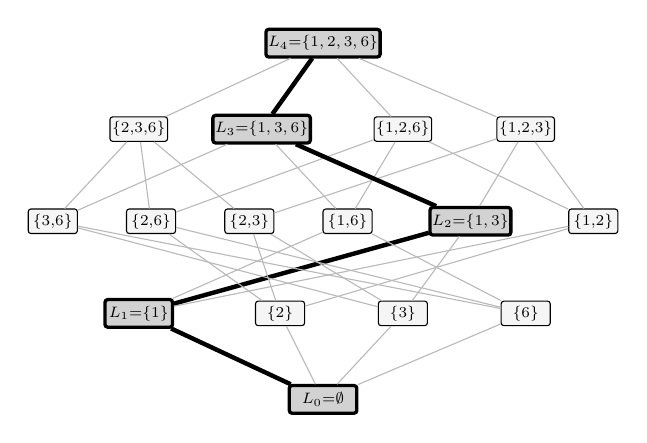
\begin{tikzpicture}[
    every node/.style={font=\scriptsize},
    pt/.style={draw, rounded corners=1pt, fill=gray!8,
               minimum width=8mm, minimum height=4mm, inner sep=1pt},
    chosen/.style={draw=black, very thick, fill=gray!35,
                   rounded corners=1pt,
                   minimum width=11mm, minimum height=4.5mm,
                   inner sep=1pt},
    edge/.style={-, thin, gray!55},
    chosenedge/.style={-, ultra thick, black},
    scale=0.78, transform shape,
]
% Layer 4 (top): L_4 = {1,2,3,6}
\node[chosen] (L4) at (4.0, 5.4) {$L_4{=}\{1,2,3,6\}$};
% Layer 3: 4 nodes; L_3 = {1,3,6}
\node[pt]     (n3a) at (1.0, 4.0) {\{2,3,6\}};
\node[chosen] (L3)  at (3.0, 4.0) {$L_3{=}\{1,3,6\}$};
\node[pt]     (n3c) at (5.3, 4.0) {\{1,2,6\}};
\node[pt]     (n3d) at (7.3, 4.0) {\{1,2,3\}};
% Layer 2: 6 nodes; L_2 = {1,3}
\node[pt]     (n2a) at (-0.4, 2.5) {\{3,6\}};
\node[pt]     (n2b) at (1.2, 2.5) {\{2,6\}};
\node[pt]     (n2c) at (2.8, 2.5) {\{2,3\}};
\node[pt]     (n2d) at (4.4, 2.5) {\{1,6\}};
\node[chosen] (L2)  at (6.4, 2.5) {$L_2{=}\{1,3\}$};
\node[pt]     (n2f) at (8.4, 2.5) {\{1,2\}};
% Layer 1: 4 nodes; L_1 = {1}
\node[chosen] (L1)  at (1.0, 1.0) {$L_1{=}\{1\}$};
\node[pt]     (n1b) at (3.3, 1.0) {\{2\}};
\node[pt]     (n1c) at (5.3, 1.0) {\{3\}};
\node[pt]     (n1d) at (7.3, 1.0) {\{6\}};
% Layer 0 (bottom)
\node[chosen] (L0) at (4.0, -0.4) {$L_0{=}\emptyset$};

% Edges layer 0 -> 1
\draw[chosenedge] (L0) -- (L1);
\draw[edge] (L0) -- (n1b);
\draw[edge] (L0) -- (n1c);
\draw[edge] (L0) -- (n1d);
% Edges layer 1 -> 2
\draw[edge]       (L1) -- (n2d);   % {1} -> {1,6}
\draw[chosenedge] (L1) -- (L2);    % {1} -> {1,3}
\draw[edge]       (L1) -- (n2f);   % {1} -> {1,2}
\draw[edge] (n1b) -- (n2b);  % {2} -> {2,6}
\draw[edge] (n1b) -- (n2c);  % {2} -> {2,3}
\draw[edge] (n1b) -- (n2f);  % {2} -> {1,2}
\draw[edge] (n1c) -- (n2a);  % {3} -> {3,6}
\draw[edge] (n1c) -- (n2c);  % {3} -> {2,3}
\draw[edge] (n1c) -- (L2);   % {3} -> {1,3}
\draw[edge] (n1d) -- (n2a);  % {6} -> {3,6}
\draw[edge] (n1d) -- (n2b);  % {6} -> {2,6}
\draw[edge] (n1d) -- (n2d);  % {6} -> {1,6}
% Edges layer 2 -> 3
\draw[edge] (n2a) -- (n3a);  % {3,6} -> {2,3,6}
\draw[edge] (n2a) -- (L3);   % {3,6} -> {1,3,6}
\draw[edge] (n2b) -- (n3a);  % {2,6} -> {2,3,6}
\draw[edge] (n2b) -- (n3c);  % {2,6} -> {1,2,6}
\draw[edge] (n2c) -- (n3a);  % {2,3} -> {2,3,6}
\draw[edge] (n2c) -- (n3d);  % {2,3} -> {1,2,3}
\draw[edge] (n2d) -- (L3);   % {1,6} -> {1,3,6}
\draw[edge] (n2d) -- (n3c);  % {1,6} -> {1,2,6}
\draw[chosenedge] (L2) -- (L3);    % {1,3} -> {1,3,6}
\draw[edge]       (L2) -- (n3d);   % {1,3} -> {1,2,3}
\draw[edge] (n2f) -- (n3c);  % {1,2} -> {1,2,6}
\draw[edge] (n2f) -- (n3d);  % {1,2} -> {1,2,3}
% Edges layer 3 -> 4
\draw[edge]       (n3a) -- (L4);
\draw[chosenedge] (L3)  -- (L4);
\draw[edge]       (n3c) -- (L4);
\draw[edge]       (n3d) -- (L4);
\end{tikzpicture}
\caption{Hasse diagram of the consistency lattice
$\mathcal{L} = \langle 2^{\{A_1, A_2, A_3, A_6\}}, \subseteq
\rangle$. Each node is the subset of anomalies excluded by that
model, with set elements abbreviated by their anomaly indices
(e.g., $\{1, 3\}$ means $\{A_1, A_3\}$). Of the sixteen points
and thirty-two cover edges, the chosen $L_n$ chain (bold) is
one of $4! = 24$ maximal chains. The remaining eleven unnamed
points are realized by the parameterized runtime of
Section~4.2 of the main paper.}
\label{fig:lattice}
\end{figure}

\begin{table}[h]
\centering
\caption{Each named lattice point on the chosen chain admits
($\checkmark$) or prevents ($\times$) each of the four formalized
anomalies. ADMITS column entries are verified by explicit TLC
counter-example traces; PREVENTS column entries follow from the
definitions of Section~4 of the main paper and are mechanically verified
by the TLAPS coherence check (Section~5 of the main paper). The eleven
unnamed lattice points are not tabulated; their admissions and
preventions follow from their subset memberships and are checked
individually in Section~4.2 of the main paper.}
\label{tab:chain}
\begin{tabular}{lcccc}
\hline
Level & $A_1$ & $A_2$ & $A_3$ & $A_6$ \\
\hline
$L_0$ & $\checkmark$ & $\checkmark$ & $\checkmark$ & $\checkmark$ \\
$L_1$ & $\times$     & $\checkmark$ & $\checkmark$ & $\checkmark$ \\
$L_2$ & $\times$     & $\checkmark$ & $\times$     & $\checkmark$ \\
$L_3$ & $\times$     & $\checkmark$ & $\times$     & $\times$     \\
$L_4$ & $\times$     & $\times$     & $\times$     & $\times$     \\
\hline
\end{tabular}
\end{table}


\smallskip
\noindent\emph{The value domain, and what widening it changes.} A
single-element $\mathit{Values}$ is the sharpest restriction in that
configuration, and it is not cosmetic: \texttt{Guarded.tla} constrains a
write to a cell of the write set to be non-\textsc{null}, so with one
non-\textsc{null} value every write writes it, and an $A_1$ witness in the
matrix can only be a read of the initial sentinel. A conflict between two
\emph{written} values is not expressible at that bound. We therefore re-ran
the safety half at $\mathit{Values}=\{v_1,v_2\}$. All $32$ safety runs
remain \textsc{safe}, over $2{,}076{,}952$ to $8{,}102{,}746$ distinct
states---a $6.1$ to $8.8${-fold} growth, since the symmetry declaration
covers agents and cells but not values---with no run exceeding a one-hour
timeout or the $6$\,GB heap. These two-value figures (tracked in \texttt{v2\_safe\_cells.txt}) were
measured on the model as it stood before $G_3$ became output commit---their
$6.1$ to $8.8$-fold growth is relative to that model's single-value counts
($342{,}120$--$941{,}970$)---and the two-value safety half has not been re-run
since; for \textsc{NoA3} it is a result about the superseded guard. The realizability claim is thus not an artifact
of the single-value domain on the side where it could have been: the four
disciplines still prevent exactly their avoidance sets when a second value
exists for them to fail on. The $32$ witness runs were not re-run, and do
not need to be: widening $\mathit{Values}$ only adds behaviours, so every
witness trace at $\mathit{Values}=\{v_1\}$ remains a trace at
$\{v_1,v_2\}$. What the wider domain does \emph{not} do is make a new
witness class reachable, and establishing that corrected an attribution we
had made earlier.

Write $\textsc{NoA1NonNullRead}$ for Definition~1 of the main paper restricted to the class a
single-value domain cannot express: the stale read observed a value another
agent had written, not the initial sentinel, and the superseding write carried
a different real value. Checking it on the unguarded configuration across both
parameters gives a complete answer:

\begin{center}
\setlength{\tabcolsep}{3.5pt}
\begin{tabular}{@{}lcc@{}}
\toprule
& $\mathit{MaxOps}{=}2$ & $\mathit{MaxOps}{=}3$ \\
\midrule
$\mathit{Values}{=}\{v_1\}$     & unreach. ($1{,}049{,}042$) & unreach. ($1{,}480{,}723$) \\
$\mathit{Values}{=}\{v_1,v_2\}$ & unreach. ($9{,}227{,}002$) & \textbf{reachable} ($14{,}976$) \\
\bottomrule
\end{tabular}
\end{center}

Both conditions are necessary and neither suffices alone. A second value is
required because with one non-\textsc{null} value the read and the superseding
write cannot differ. Three operations are required because
\texttt{Memory.tla} constrains a read to observe memory
($\neg\mathit{AllowSkew} \Rightarrow \mathit{rv} = \mathit{memory}$) and memory
begins all-\textsc{null}, so the witness needs a seeding write, the
superseding write, and the reader's own commit---three entries in a log that
$\mathit{MaxOps}=2$ caps at two. We had previously attributed the limitation
to the value domain alone; the table shows that is wrong, and the
sixteen-point matrix is bounded on the witness side by
$\mathit{MaxOps}$. The safety side, which is what realizability
asserts, is unaffected: all $32$ safety runs hold at
$\mathit{Values}=\{v_1,v_2\}$ as reported above.

\medskip
\noindent\textbf{Interaction, characterized.}
The matrix is also the interaction analysis. At the safety level the four
disciplines do not interact: because the carriers are disjoint, enabling
one guard neither creates nor removes any other anomaly---$G_3$'s
cascading retractions induce no stale generation, phantom tool, or
reordering, and $G_1$'s refusals induce no uncompensated cascade---and the
check confirms this on every one of the $2^4$ combinations rather than on
the single three-way composition of Section~5.4 of the main paper. The interaction
that does exist is at the cost level: a guard prevents by refusing a
commit, a refused commit is a lost generation, and the lost generations are
the abort-rate envelope of Section~6.6 of the main paper. Whether one guard's
refusals raise another's---sequencing lengthens the window in which
validation can fail---is a cost measurement, not a safety question, and is
the empirical follow-up.

\medskip
\noindent\textbf{Scope.}
This is bounded model checking at small parameters, in the same sense as
the witnesses of Section~3 of the main paper: witness traces embed upward into
larger configurations; the safety runs are exhaustive within the bounds,
not proofs. The Verus product of the $L_2$, $L_3$, and $L_4$ models
(Section~5.4 of the main paper) mechanizes the all-enabled point; extending that
product with the four switches is the proof-level follow-up. The
\VerusCurated-obligation headline of Section~5.2 of the main paper does not include
these runs.

% =====================================================================

\section*{Appendix M: Synthetic pilot; cost Findings 1--5 and the inference-cost sweep}

\subsection*{Workload}
The pilot uses seven synthetic but reproducible task scenarios
designed to surface specific points in the lattice:
\begin{itemize}
    \item \textbf{Concurrent stale-read.} Two agents read the same
    cell at the same clock tick, then commit divergent values in
    different orders. Designed to surface $A_1$.
    \item \textbf{Tool deprecation.} An agent plans a tool at
    \texttt{begin}; the tool is removed from the registry before
    \texttt{commit}. Designed to surface $A_2$.
    \item \textbf{Phantom-write cascade.} An agent reports having
    read a value of $c$ that no committed write produced---a
    commit-log skew. Designed to surface the flat-trace residue of
    Appendix~G; the synthetic traces carry no provenance or
    externalization fields, so Definition~4 of the main paper itself is not decidable on them.
    \item \textbf{Tool-effect reorder.} An agent issues writes in
    order $[x, y]$ but the store commits them in order $[y, x]$,
    simulating asynchronous tool execution. Designed to surface
    $A_6$.
    \item \textbf{Linear pipeline (clean).} Three agents update a
    shared progress cell in strict sequence. Control: no anomaly
    expected.
    \item \textbf{Fan-out merge.} A coordinator forks two workers
    writing disjoint cells, then merges. Branching control with no
    shared write target.
    \item \textbf{Single-agent control.} One agent makes three
    sequential updates. Single-agent control: no anomaly possible.
\end{itemize}
We executed 700 trace generations with scenarios drawn uniformly at
random under a fixed seed, producing 700 JSON Lines traces. The first
four scenarios are designed to surface one anomaly each; the
remaining three are controls with no anomaly expected.


\paragraph{Witness classes, and the further runs.}
The 100\% rate in
edit-review is structurally guaranteed by workload design, and the mechanism
is worth naming because it is not the one the narrative of
Section~1.1 of the main paper suggests. Classifying every committed
Definition~1 of the main paper witness by what the stale read actually observed
(\texttt{python/witness\_classes.py}) splits them in two: a \emph{cold-start}
witness read the store's initial sentinel, so the reader reached the cell
before anyone had written it, while a \emph{supersession} witness read a value
another agent wrote and had it overwritten inside its window. All $300$
edit-review-vanilla witnesses across the three runs are cold-start, and
$94.2\%$ of the synthetic pilot's $485$ witnesses are. The live study of
Section~6.1 of the main paper is the opposite: all $292$ of its witnesses are
supersessions. The two halves of the empirical section therefore exercise
different witness classes, and the synthetic rates should not be read as
smaller-scale measurements of what the live study measures. The same split
bounds the formal side, though not for the reason we first recorded. At
$|\mathit{Values}|{=}1$ the lattice matrix of Section~4.2 of the main paper can indeed
express only the cold-start class, since a write to a cell in the write set is
constrained non-\textsc{null} and one non-\textsc{null} value leaves a
supersession with nothing to differ from. But widening the domain does not by
itself reach the other class, and Section~4.2 of the main paper reports the check that
shows why: the binding constraint is the operation budget, not the value
domain. Plan-execute is
0/100; the 42\% in triage is the only non-trivial intermediate
measurement. Two further independent runs of the same protocol give edit-review
100/100 and 100/100, plan-execute 0/100 and 0/100, and triage 52/100 and
48/100; these are \texttt{20260913T0128Z} and the vanilla column of the
Table~4 of the main paper run \texttt{20260913T0150Z}, both committed
with their traces; pooled over the three runs, triage is
$142/300$ [41.6, 53.2].

Table~4 of the main paper reports the level distribution. Three
findings.

First, the edit-review rate of 100\% confirms that under
round-robin scheduling with both agents required to read the same
cell before either writes, $A_1$ is \emph{structurally guaranteed}
rather than empirically observed. We retain this workload in the
table not as a measurement of $A_1$ prevalence in the wild but as a
calibration point: the rate at which the LLM follows the prescribed
2-call (read, write) pattern, with the residual 0\% accounted for
by sessions in which the model collapsed reads and writes into a
single turn.

Second, the plan-execute rate of 0\% ($0/300$ pooled over three runs,
[0, 1.2]) confirms that strictly sequential workflows --- where no cell
is concurrently readable by two agents whose writes follow --- suppress
$A_1$; an earlier run reported a single firing that the regenerated
traces do not reproduce.

Third, the triage rate of 42\% (48\% and 52\% in two further runs;
$142/300$ pooled) is the only measurement of the three that occupies a
non-trivial intermediate regime. The 3-agent pipeline produces $A_1$
when the engineer's read of \texttt{ticket} interleaves with the
triager's still-active read window, but not always; the variability comes
from the LLM's tool-call ordering within each agent's turn, and the
run-to-run spread at a fixed harness seed is the sampling variance of
the model, which the seed does not pin.


\subsection*{Synthetic baseline comparison}
To check whether the rates above are artifacts of an unguarded runtime, we
re-ran the 700-trace synthetic pilot through three variants (vanilla;
pessimistic locking, on-conflict ops silently dropped; snapshot isolation,
on-conflict commits aborted) on the same scenarios, seed, and detector
pipeline. Pessimistic locking drives both $A_1$ and $A_2$ to $0\%$ at the
cost of 285 dropped operations (40.7\%); snapshot isolation drives $A_1$ to
$0\%$ but leaves $A_2$ at $21.1\%$ (its scope is value memory, not the tool
registry) at 145 aborts (20.7\%); vanilla exhibits $A_1$ at $20.7\%$ and
$A_2$ at $21.1\%$ with no aborts. Under these scripted scenarios both
guarded runtimes pay $\geq 1$ abort per anomaly prevented, and a
sound-and-complete detector returning $L_4$ is machine-checkable evidence
of an anomaly-free trace. This controlled-scale result is superseded by the
LLM-scale baseline of Section~6.2 of the main paper, where each drop or
abort corresponds to a re-issued inference call.

\paragraph{Observation: snapshot isolation's classical incompleteness manifests in the agent setting.}
The SI runtime validates a committing operation against concurrent writers
to its read set \emph{at commit time}, but validation triggers only on a
non-empty write set; a read-only operation ticks the clock and emits a
no-write $\fld{OpRecord}$ without validation. This is the classical
write-only SI behavior---read-only transactions in textbook SI are not
validated~\citep{CahillRohmFekete2008SSI,FeketeEtAl2005MakingSI}, and
read-set serialization (SSI) closes the gap. We did not implement SSI in
the pilot (a deliberate scope choice); the residuals are the fraction of
sessions in which a read-only operation's decision reaches downstream
agents without materializing as a validated write, not a general claim.
Concretely, in each of the five edit-review residuals the reviewer's
no-write commit at $t=2$ follows the editor's write at $t=1$ that landed
inside the reviewer's window opened at $t=0$; in the eight triage
residuals the reporter writes the ticket twice and the triager or
engineer, having read the first version, commits without writes against
the second. The conceptual content---read-only operations
that influence downstream agents need SSI-style validation---is identical
to the database case; the operational regime in which it matters is what
is new.

\paragraph{Pessimistic locking eliminates $A_1$ in every cell, by
dropping the contested operation.}
The pessimistic-locking runtime drops every conflicting operation
silently (Appendix~M), and every cell of
Table~4 of the main paper shows zero $A_1$ instances---because in
edit-review the reviewer's operation is gone in 99 of 100 sessions and in
triage one of three agents' operations is gone in 95 of 100. The
mechanism is stronger than SI's because the lock is acquired \emph{before}
the operation reads, and a failed acquisition drops the operation without
invoking the LLM beyond the agent's planning phase; what it prevents is
the stale commit, and what it costs is the second agent's contribution.
It is the right mechanism only where a dropped contribution is
acceptable and a wasted inference is not; where the contribution must
survive, the $L_1$ discipline that keeps it is validation with retry (SSI,
Section~5.2 of the main paper), whose cost is the re-spent generation of
Section~6.6 of the main paper.

\paragraph{Cost of prevention.}
Both disciplines drop a substantial fraction of operations under
contention. Scored on the committed traces
(\texttt{python/task\_utility.py}), in edit-review pessimistic locking drops
the reviewer's commit in $99\%$ of sessions and default-SI in $95\%$, though
the LLM inference still ran (SI aborts at validation,
pessimistic fails acquisition---which could in principle short-circuit the
call but does not in our implementation).

\smallskip
\noindent\emph{Prevention scored on the outcome, not on the anomaly rate.}
A discipline can drive the anomaly rate to zero by refusing every contested
commit, and a token metric records that as cheap. We therefore score each
cell on three quantities: \emph{clean} (no Definition~1 of the main paper witness),
\emph{complete} (every role that commits in the unguarded cell of the same
run also commits here---derived from the baseline rather than declared), and
\emph{both}. On edit-review the unguarded baseline is complete $100/100$ and
clean $0/100$; pessimistic locking is clean $100/100$ and complete $1/100$;
default-SI is clean $95/100$ and complete $5/100$, and those five are exactly
the five that fired, so on this workload the reviewer's contribution reaches
the log \emph{if and only if} it is stale. No discipline, including the
baseline, delivers more than one complete-and-clean session out of a hundred
there. On triage the picture differs and is worth stating against our own
recommendation: default-SI is complete-and-clean in $45/100$ while the
unguarded baseline is in $52/100$, because default-SI drops the engineer in
$47\%$ of sessions. Only plan-execute, which aborts nothing, is unaffected.
\emph{Complete} is a structural proxy---it counts whether the baseline's set
of contributors reappears, not whether a human would call the task done---and
a session missing one role may still be useful output. With that caveat, a
prevention claim should be read against \emph{both}, and the main paper's discussion's
recommendation of snapshot isolation should be read as workload-dependent
rather than general. A defensible cost claim requires
per-session token counts from the client \texttt{usage} callbacks, which
the original pilot did not capture (character-derived estimates
underestimate cost by ignoring history growth and intermediate tool-call
exchanges). We measure token-level cost at LLM scale in
Section~6.6 of the main paper.


\medskip
\noindent\textbf{Finding 1: between sessions, snapshot isolation's token cost
is not separable from the unguarded runtime's.}
The SSI mean sits within sampling noise of vanilla in every cell: CIs overlap
on edit-review (3.11 vs 3.13), plan-execute (1.95 vs 1.93), and triage (3.13
vs 3.23). This is a statement about a per-session denominator, which credits a
discipline for work it declined to do; Finding~6 re-prices the same run per
sound committed operation, and the parity does not survive. An earlier version
cited here a paired ${\sim}8\%$ overhead on plan-execute. That figure comes
from the study of Appendix~O, whose aborts are injected at a fixed
probability; the real store never aborts on plan-execute, so the figure prices
the injection and not the discipline, and we no longer cite it as a cost of
snapshot isolation. The $A_1$-prevention
rate of the pilot's default-SI store is 95\%, 100\%, and 92\%
respectively (Table~4 of the main paper); the SSI mode of the Rust
runtime (Section~5.2 of the main paper), which validates read-only commits,
is the mechanism the cost figures should be read against. The classical cost asymmetry that
motivates serializable snapshot isolation in the database setting
\citep{CahillRohmFekete2008SSI}---validation rather than locking keeps
reads non-blocking---transfers to the agent setting in the form most
favorable to deployment.

\medskip
\noindent\textbf{Finding 2: pessimistic locking incurs bounded
overhead, concentrated in multi-stage contention.}
On edit-review the pessimistic overhead is statistically zero
(CIs marginally overlap: 3.21--3.38 vs 3.11--3.16). On
plan-execute the overhead is also zero (slightly cheaper than
vanilla, within noise). On triage the overhead is real and
statistically significant: \$5.21\,m vs \$3.23\,m, with CIs
[4.90, 5.54] vs [2.93, 3.55] that do not overlap, an
$\approx$62\% increase. The pattern matches Appendix~M: pessimistic locking
adds cost where lock contention forces wait-and-retry across pipeline
stages, and is essentially free in single-writer or low-overlap
workloads.

\medskip
\noindent\textbf{Finding 3: the cost asymmetry in the agent
setting is bounded at $\leq$1.6\,$\times$ vanilla in the worst
measured workload on gpt-4o, not the unbounded "orders of
magnitude" that Section~2 of the main paper speculated.}
Our pre-measurement intuition---that a discarded LLM inference is
"cripplingly expensive"---is empirically wrong for these workloads at
this scale: worst-case overhead is bounded, typical-case near zero.
Abort costs remain non-trivial in kind (Appendix~M:
pessimistic locking drops 40.7\% of synthetic operations), but not
order-of-magnitude in measured cost.

\medskip
\noindent\textbf{Cross-model validation on Claude Sonnet 4.5.}
To probe whether the gpt-4o findings reflect properties of the
runtime model or of one specific model family, we replicated
the full 900-session protocol against Anthropic's
\texttt{claude-sonnet-4-5-20250929}, identical workloads and
identical instrumentation. Table~S2 (this appendix) reports the
per-session cost. Claude pricing at the time of the run is
\$3.00/M input tokens, \$15.00/M output tokens.

\smallskip
\noindent\textbf{Rerun with operation records (run
\texttt{20261014T0253Z-claude}, 2026-10-14).} The replication above
predates the operation recorder, so its sessions carry no \A1 verdict. The
vanilla column was rerun on \texttt{claude-sonnet-4-5} with the recorder
on, $100$ sessions per workload, seed $42$, and scored under Definition~1 by
the same scorer as the gpt-4o cells: edit-review $100/100$ (the forced
overlap, as on gpt-4o), plan-execute $0/100$ (the sequential control).
Per session the vanilla cells cost $4{,}315$ and $2{,}504$ tokens
($\$0.0162$, $\$0.0094$; $8.3$\,s and $4.8$\,s wall-clock) against $1{,}016$
and $620$ tokens on gpt-4o, the model answering at greater length in five
and three calls respectively. The triage cell is \emph{void}: in $100/100$
sessions the reporter wrote a ticket reading ``no bug description provided''
and the triager and engineer wrote nothing, so no operation of the pipeline
could overlap a write; the same harness delivered the ticket text to
gpt-4o's reporter (run \texttt{20260913T0150Z}: $17$ distinct trace shapes,
\texttt{priority} written in $28/100$ sessions). Whether the description was
dropped by the provider adapter or declined by the model is not resolved by
these records, and the cell is reported as void rather than as $0/100$. The
guarded cells (pessimistic, snapshot isolation) of this rerun did not
execute (an import path broken by the repository migration) and remain
listed as not run in the main paper. All $750$ records pass the H0/H1 gates
(\texttt{hypothesis\_gates}: $0$ overlaps, $0$ read-after-commit).


\medskip
\noindent\textbf{Finding 4: SSI between-session cost-parity replicates
across model families; pessimistic-overhead pattern is
qualitatively consistent, quantitatively model-dependent.}
The strongest claim in this section---that snapshot isolation
adds no cost overhead detectable between sessions vs vanilla---
holds in both model families. All six SSI cells (three
workloads $\times$ two providers) have means within sampling
noise of their vanilla counterparts: CIs overlap on every cell.
Pessimistic overhead retains the same shape on both providers
(approximately zero on edit-review and plan-execute, real
overhead concentrated in triage), but the magnitude of the
triage overhead scales differently: gpt-4o exhibits a 62\%
overhead in triage-pessimistic, while Claude Sonnet 4.5
exhibits a 124\% overhead in the same cell (
$\$27.73$\,m vs $\$12.36$\,m vanilla, non-overlapping CIs).
Wall-clock latency follows the same pattern: triage-pessimistic
on Claude requires 21.4\,s median wall-clock vs 10.5\,s
vanilla, a 2$\times$ latency penalty matching the cost penalty.
The magnitude difference is not explainable from these data alone
(candidate mechanisms: retry budgets, client-side tool serialization,
tokenization density); the qualitative conclusion stands on both
providers---bounded, $\leq$1.6$\times$ (gpt-4o) to $\leq$2.3$\times$
(Claude), never order-of-magnitude.

\medskip
\noindent\textbf{Finding 5: SSI costs one re-spent generation per abort,
and a re-spent generation costs $1.074\times\,[1.052,1.096]$ a first-attempt
one.}
To test the discipline where its abort-and-retry machinery engages, we ran
a paired high-contention sweep (\Cref{fig:cost-envelope}): contention
varied two independent ways---fan-in $W \in \{2,4,8,16\}$ at one cell, and
cell count $C \in \{2,4,8,16,32\}$ at $W{=}8$---over 155 paired sessions on
gpt-4o-mini at realized abort rates $0.09$--$0.93$. Token cost is counted
exactly (including generations re-spent on aborts), and the harness
re-verifies per session that the baseline exhibits $A_1$ while the guarded
disciplines do not---scored with the superstep form of the predicate
(Appendix~C), since each round of the sweep is a single
superstep whose commits land at one tick---so the measured quantity is the
cost of \emph{working} prevention.

\smallskip
\noindent\emph{What in this sweep is arithmetic.} Regressing token overhead
on the realized abort rate returns
$+0.1\% + 108\%\times\text{abort\_rate}$ at $R^2 = 0.94$, and that
regression is an accounting identity rather than a result. The committed
sessions show why: in all $155$ SSI sessions the harness records
$\mathit{generations} = W\!\cdot\!\mathit{depth} + \mathit{aborts}$, and in
all $155$ vanilla and $155$ pessimistic sessions
$\mathit{generations} = W\!\cdot\!\mathit{depth}$. The realized abort rate
$\mathit{aborts}/(W\!\cdot\!\mathit{depth})$ is therefore exactly
\emph{extra generations per baseline generation}, while token overhead is
extra tokens per baseline token; regressing the second on the first
recovers one quantity only---the price of a retried generation relative to
a first-attempt one---and the $R^2$ measures how tightly tokens track
generations, not how well a law fits. The collapse of the two contention
mechanisms onto a common line is forced for the same reason: any mechanism
that produces aborts lands there.
\texttt{python/fig\_cost\_envelope.py -{-}stats-only} prints the identity
check and every figure below.

\smallskip
\noindent\emph{What the sweep establishes.} Four things the identity does
not force. \emph{(i)} The fitted intercept is indistinguishable from zero
($+0.05\%$, $95\%$ CI $[-1.5,+1.7]$), and the eight sessions that aborted
not at all cost $+0.56\%$ in the mean: SSI carries no fixed overhead, only
a per-abort one. \emph{(ii)} The per-abort price does not steepen with
contention---below abort rate $0.5$ the slope is $110.7\%\,[99.8,121.4]$
and above it $106.5\%\,[97.5,115.2]$---so aborts do not compound, which a
discipline that re-validated a growing read set on every retry would not
satisfy. \emph{(iii)} The two contention mechanisms agree on the per-abort
price in absolute tokens ($1.077\,[1.05,1.11]$ for the fan-in sweep,
$1.071\,[1.04,1.10]$ for the cell-count sweep), so the retry price is a
property of the discipline rather than of how contention is induced.
\emph{(iv)} A retried generation costs $1.074\times$ a first-attempt one
($95\%$ CI $[1.052,1.096]$, bootstrap over the $147$ sessions with at least
one abort): re-prompting after a refused commit is measurably dearer than
the original attempt, because the retry carries the conflict into its
prompt. That ratio is the entire empirical content of the $108\%$ above,
and \Cref{fig:cost-envelope}B shows it directly, against the null in which
a retry costs exactly one generation.

\smallskip
\noindent The practical envelope follows from \emph{(i)}--\emph{(iv)}
rather than from the regression: overhead is zero when nothing aborts and
$1.074$ generations per abort thereafter, so it reaches $15\%$ at an abort
rate of $0.14$---which is $0.15/1.074$, arithmetic on the measured retry
price and not a fitted breakpoint. The lowest cell measures
$+9.9\%\,[5.6,14.5]$ at abort rate $0.09$, so that regime is measured
rather than extrapolated, and what it measures is low overhead, not zero.
We do not establish that deployed workloads occupy it (the corpus audit of
Appendix~C is consistent with it but is not an abort-rate
measurement); the envelope instead makes the question auditable per
deployment. Pessimistic locking is the complementary profile:
token-neutral between sessions ($\pm1\%$) but serializing critical
sections, so its cost is real yet invisible to a token metric (wall-clock
figures here are \emph{composed} from per-call latencies, not measured
under a live concurrent runtime, and grow several-fold at $16$-way).

\begin{figure*}[t]
\centering
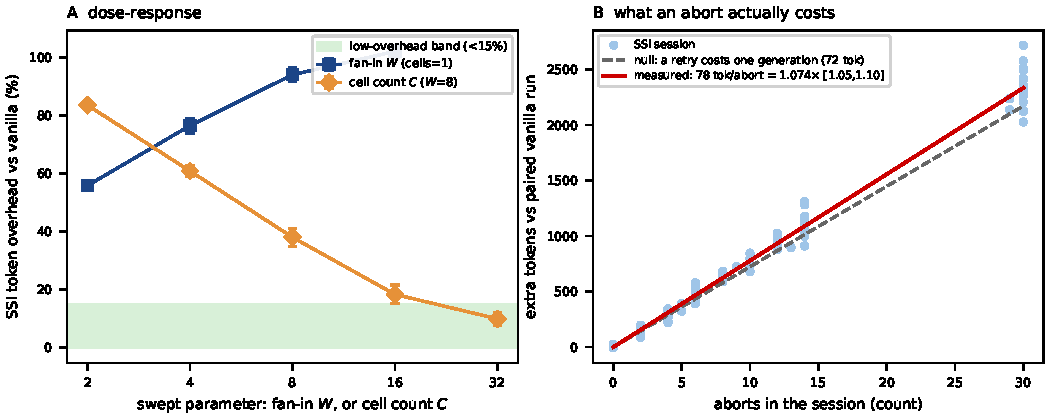
\includegraphics[width=0.86\textwidth]{fig_cost_envelope.pdf}
\caption{The high-contention sweep (gpt-4o-mini, 155 paired
sessions), separated into what the accounting identity forces and what
the data measures. \textbf{A}: mean SSI token overhead against the
parameter we \emph{set}---fan-in $W$ at one cell (squares) and cell count
$C$ at $W{=}8$ (diamonds), error bars $\pm1$ s.e.---rather than against
the realized abort rate, which is another outcome of the same runs. The
two knobs move overhead in opposite directions and the sweep crosses the
low-overhead band (${<}15\%$; a descriptive plotting threshold---the
pre-declared equivalence margin of Appendix~O is the stricter
$\pm10\%$). \textbf{B}: extra tokens against aborts in absolute units.
The dashed line is the null in which a retried generation costs the same
as a first-attempt one ($72$ tokens); the fitted line is the measurement,
$78$ tokens per abort, a ratio of $1.074\,[1.052,1.096]$. The gap between
the lines is the only quantity the former $108\%$ slope carried.
Pessimistic locking is token-neutral in between-session means but incurs the wall-clock
cost reported in the text. Regenerate with
\texttt{python/fig\_cost\_envelope.py}.}
\label{fig:cost-envelope}
\end{figure*}


\medskip
\noindent\textit{What this section cannot establish.}
The measurement covers gpt-4o and Claude Sonnet 4.5 on these
three workloads. Cost behavior on Gemini or other providers, and
on workloads with materially larger read-sets, is not measured;
the high-contention sweep of Finding 5 covers fan-in up to 16
agents and multi-round pipelines, but only on gpt-4o-mini. The measured cost asymmetry is consistent with the
design intuition that SSI offers a near-optimal cost-correctness
trade-off in low-to-moderate contention regimes and pessimistic
locking is preferable only under workload-specific contention
patterns; the two-provider replication strengthens this claim
qualitatively but does not generalize to open-weights models or
to model families optimized for low-latency tool use. Three-plus
provider replication including local open-weights inference
(Llama, Mistral) and higher-contention workload exploration are
identified as principal empirical follow-up
(Section~8 of the main paper).


\section*{Appendix N: Operational materiality: table, scope and the advisory layer}

\begin{table}[t]
\centering
\caption{Operational disagreement probability $p_{\text{op}}$: fraction of
flagged events that change the agent's decision. The controlled task uses
an exact categorical comparator; pilot-trace free-text outcomes are
LLM-judged at decision level (a softer signal). All pilot events are
read-before-write ($v_{\text{stale}}=\textsc{null}$). Only the reviewer
row is scored on Definition~1 of the main paper firings; the engineer and editor rows are
scored on later-rewrite events (the rewrite landed after the reader's
commit), which the corrected predicate does not classify as $A_1$.}
\label{tab:operational-materiality}
\small
\footnotesize
\begin{tabular}{@{}llcc@{}}
\toprule
Setting & Role / decision & $p_{\text{op}}$ & 95\% CI \\
\midrule
Controlled & triage priority (categorical) & 75.0\% & [68.4, 80.8] \\
Pilot ($A_1$)  & reviewer (assess doc)      & 100\%  & [91.8, 100] \\
Pilot (later rw.) & engineer (resolve, judged) & 54.5\% & [36.4, 71.9] \\
Pilot (later rw.) & editor (author, judged)   & 0\%    & [0, 3.6] \\
\bottomrule
\end{tabular}
\end{table}

\paragraph{Scope.} The controlled task is a proxy with an exact
comparator; deployed free-text outcomes are judged by an LLM of the same
family under a decision-level rubric and are reported as a softer,
corroborating signal. On a blind sample of 60 judged firings---the
coder shown only the two free-text outputs, not the model's
verdict---manual coding agreed with the LLM judge on 59 of 60
($98\%$; Cohen's $\kappa=0.96$ between judge and human, approximate
95\% CI $[0.89, 1.00]$), so the judge tracks a human reading of
decision-level divergence rather than a lexical artifact. We state the sample's composition rather than let it
be inferred: those 60 rows are 35 editor, 10 engineer and 15 reviewer
events, so 45 of them belong to the later-rewrite class this subsection
withdraws, and only 15 of the reviewer's 43 genuine firings were blind
coded. The agreement figure is therefore evidence that the judge tracks
human decision-level reading in general, not a validation restricted to
the 43; re-coding those 43 is outstanding. All pilot firings are read-before-write,
so value-staleness is exercised only by the controlled experiment. The
editor and engineer results reflect these workloads, in which the
producer does not fully consume the read; they are not a claim that
producer roles are universally immune. The triager cell had only three
qualifying firings, too few to estimate a rate, and is omitted from
\Cref{tab:operational-materiality}.

\paragraph{Design consequence: an advisory materiality layer over the
verified core.} The controlled result---one flagged mismatch in four did
not change the decision---bears directly on the objection that a boolean
detector firing can be operationally meaningless. The verified core remains
the boolean predicate of Section~5.1 of the main paper; we do not weaken its
sound-and-complete guarantee. A deployment can wrap it in an \emph{advisory}
pair $(\textit{detected},\,\hat{p}_{\text{op}})$, with
$\hat{p}_{\text{op}}$ estimated per prompt by the counterfactual re-prompt of
this section, so that an abort policy gates on $\hat{p}_{\text{op}}>\theta$
rather than on the raw firing. An earlier version proposed estimating
$\hat{p}_{\text{op}}$ from the firing agent's \emph{role}; the role-dependence
that rested on is withdrawn above, and the knob is withdrawn with it. The
layer is deliberately unverified and outside the trust base: it changes which
firings a runtime \emph{acts} on, not which the verified detector
\emph{reports}.

% =====================================================================

\section*{Appendix O: The injected-abort wall-clock study}

\subsection*{Within-model wall-clock study (injected aborts)}

The token-instrumented cost study of Section~6.6 of the main paper
reports relative overhead within each provider but invites the
objection that any comparison \emph{across} providers conflates
runtime overhead with tokenization, pricing, and serialization
differences, and that billed tokens are not the same quantity as
wasted wall-clock computation. This subsection reports the
instrument we identified as the clean resolution: a study that
holds the model fixed (gpt-4o), varies only the runtime
strategy, and measures \emph{wall-clock seconds} rather than
billed tokens.

\medskip
\noindent\textbf{Method.}
We ran 270 sessions
(\texttt{python/wallclock\_cost\_study.py}): three workloads
(edit-review, plan-execute, triage) $\times$ three strategies
(vanilla, pessimistic with a 20\% per-write abort probability,
SSI with a 5\% commit-time abort probability) $\times$ 30
sessions, on gpt-4o (and replicated on open-weights Llama-3.2 below) with
deterministic mock tools so that
the measured wall-clock isolates LLM-inference and
abort-and-retry time from external-service latency. We report
bootstrap 95\% confidence intervals (5000 resamples) on the
per-cell mean wall-clock.

\smallskip
\noindent\emph{The aborts in this study are injected.} Each strategy is
simulated by wrapping the workload's tools so that a write fails with the
stated fixed probability and is retried, independently of contention; neither
store of Section~5.2 of the main paper runs. The study therefore measures what a
retry costs, in wall-clock and in tokens, at abort rates we chose. It does not
measure the abort rate either discipline produces, and no comparison between
the two strategies' overheads can be read from it, since the $20\%$ and $5\%$
are inputs.


\medskip
\noindent\textbf{Finding.}
The wall-clock overhead of both guarded strategies over vanilla
is small and \emph{not statistically separable from
API-latency noise at $n=30$ in any of the three workloads}:
every pessimistic and SSI confidence interval overlaps the
corresponding vanilla interval. The directional pattern is
nonetheless the expected one. The overhead is largest where a session makes the most writes and so draws
the most injected aborts---triage, in which the $20\%$ injection produced 14
aborts across 30 sessions versus 6--7 in the other workloads---and the triage pessimistic interval ([4.82, 5.49])
sits almost entirely above the vanilla interval ([4.57, 5.07]),
a $+6.6\%$ point estimate. The within-cell token overhead
mirrors this: $+5.6\%$ on triage, $+3.4\%$ on edit-review,
$-1.4\%$ on plan-execute. The two apparent inversions where a
guarded strategy is point-faster than vanilla (edit-review
pessimistic and SSI) are artifacts of API-latency variance:
vanilla drew several high-latency outliers, and the strategies
do near-identical compute when realized abort counts are low.

\medskip
\noindent\textbf{What this resolves, and what it does not.}
The within-model design removes the cross-provider confound by construction:
every comparison in Table~S5 (this appendix) holds gpt-4o fixed, so
tokenization, pricing, and serialization differences cannot enter. And
measuring wall-clock rather than billed tokens addresses the ``tokens are not
wasted computation'' objection for the quantity measured: the real-time price
of retry at the injected rates is single-digit-percent and at the noise floor,
smaller than the billed-token figures, because the additional tokens of a
retried operation are largely cached-prompt context that is processed quickly
relative to a fresh generation. The conclusion is correspondingly narrow: at
injected abort rates of up to $0.47$ per session, retry imposes no wall-clock
cost separable from inference noise at $n=30$. Whether the stores' \emph{real}
abort rates on these workloads fall in that range is answered by
Table~3 and Table~4 of the main paper, not here, and on edit-review they
do not: the reviewer's commit is refused in $95$--$99\%$ of sessions.

\medskip
\noindent\textbf{Open-weights replication (Llama-3.2).}
We re-ran the identical 270-session protocol on open-weights Llama-3.2
served locally through Ollama, where dollar cost is negligible and
wall-clock is the only meaningful unit (Table~S6 (this appendix)).
Per-session wall-clock is an order of magnitude larger than on gpt-4o
(local inference at $24$--$38$\,s versus $5$--$9$\,s), and against that
latency the abort-and-retry overhead of both guarded strategies is
invisible: every pessimistic and SSI interval overlaps the corresponding
vanilla interval, with point ratios in $[0.82, 1.04]\times$ and SSI
point-faster than vanilla in all three workloads---an artifact of the large
per-call latency variance, not a real speed-up. The open-weights result
extends the noise-floor conclusion to a third model family: at the
injected abort rates, retry imposes no wall-clock cost separable from
inference noise on local Llama-3.2 either.


\medskip
\noindent\textbf{Scope.}
This is a two-model-family ($n=30$ per cell each) study with mock
deterministic tools; its aborts are injected rather than produced by the stores, and it does not capture real-tool latency, and at $n=30$ the API-noise floor
exceeds the overhead signal, so the study bounds the overhead
from above rather than resolving its exact magnitude. A
higher-contention workload, larger $n$, or real external tools
would be required to separate the triage signal from noise.
The \texttt{wallclock\_results.json} output is in the artifact
bundle.

\medskip
\noindent\textbf{Paired re-analysis and power.}
These are the injected-abort sessions above, so every overhead below is the
price of the injected retries, not of a store. Because the same per-session
seed was used under each strategy, a paired analysis (matched on $\langle$workload, seed$\rangle$) removes
between-session variance and yields an explicit MDE at $\alpha{=}0.05$,
power $0.80$. On \emph{token} cost it separates two small overheads from
zero---SSI on plan-execute ($+91$ tokens, ${\sim}8\%$, $[+32,+150]$,
$p{=}0.007$) and pessimistic on triage ($+41$ tokens, ${\sim}5.5\%$,
$p{=}0.04$, nominal only: not surviving Holm correction across the six
tests)---while pessimistic-on-plan-execute and SSI-on-triage are genuine
nulls (MDE $\approx 54$--$87$ tokens, below the $10\%$ effect of interest),
established as \emph{equivalent} by a two-one-sided test against the
pre-declared $\pm10\%$ margin. SSI-on-plan-execute is \emph{not} equivalent
($90\%$ CI $[+40,+140]$ vs.\ a $111$-token margin: up to ${\sim}12.6\%$),
and edit-review is underpowered (MDE $\approx 290$ tokens). On
\emph{wall-clock} time the paired MDEs ($0.7$--$3.4$\,s) exceed the
candidate effects and the lone nominal cell is in the cost-\emph{reducing}
direction (residual latency confounding), so we claim neither overhead nor
equivalence there. The paired analysis thus quantifies the earlier
statement: the token price of the injected retries is $\leq 8\%$ where separable, and
their wall-clock price is below the resolution of an $n{=}30$ design.


\section*{Appendix P: $L_2$ measurement, \texttt{ToolNode} and cost-metric notes}

\begin{table}[t]
\centering
\caption{The $L_2$ measurement on $1{,}000$ seeded schedules per depth
(\texttt{examples/l2\_measure.rs}; main paper, Section~6.3). Every figure is
decided by the schedule and the store; none is an estimate. Exposed effects:
count (scenarios).}
\label{tab:l2}
\footnotesize
\setlength{\tabcolsep}{3.5pt}
\begin{tabular}{@{}llrrr@{}}
\toprule
 & Arm & depth 2 & depth 3 & depth 5 \\
\midrule
Definition 4 (of 1000) & verified & 0 & 0 & 0 \\
 & unguarded & 519 & 624 & 563 \\
 & cascade   & 519 & 624 & 563 \\
Surviving-dependent (of 1000) & cascade & 0 & 0 & 0 \\
\midrule
Exposed effects & verified  & 402 (199) & 547 (199) & 549 (199) \\
 & unguarded / cascade & 1{,}538 (771) & 2{,}059 (771) & 2{,}010 (771) \\
Relabeled after release & cascade & 767 & 1{,}288 & 1{,}239 \\
Release refused at least once & verified & 748 & 1{,}255 & 1{,}272 \\
\quad of which released on approval & verified & 184 & 315 & 383 \\
Committed-and-unaborted released & verified & 2{,}870/2{,}870 & 3{,}494/3{,}494 & 5{,}545/5{,}545 \\
\bottomrule
\end{tabular}
\end{table}

\smallskip
\noindent\emph{What erasure costs the caller, and what the runtime now does
about it.} Under plain \texttt{cargo} every \texttt{requires} clause of the
exec API disappears, so a caller that breaks one corrupts the runtime
silently. An earlier version of this section stated that limitation and
discharged the obligations in the measurement driver. The runtime now
discharges them itself: every mutating entry point checks its own
precondition and refuses instead of assuming. \texttt{begin} returns
\texttt{Option}; \texttt{write}, \texttt{read}, \texttt{commit},
\texttt{abort} and \texttt{externalize} return whether they acted;
\texttt{commit} decides \texttt{commit\_valid} with the verified
\texttt{can\_commit} rather than trusting the caller; and each contract
states both that the return value equals the exact guard and that a refusal
leaves the abstract state unchanged. The only remaining precondition is
\texttt{wf()}, the type invariant the API itself maintains. What is still
trusted is stated in the trust base: the runtime's fields are \texttt{pub},
so a caller that writes them directly is outside what is verified.


Three properties of those figures are worth stating rather than leaving to
be checked. The baselines fail \emph{often but not always}: a baseline that fails in every scenario would make the comparison a tautology, and the
earlier $1000/1000$ was exactly that. The gate refuses in every cell, so the
freshness check is exercised rather than inert---under the previous schedule
it refused nothing at all, and a correct gate and a gate with no check were
therefore indistinguishable in the measurement. And a differential
regression test pins the difference directly: on a read-modify-write
schedule the superseded carve-out gate accepts a commit that
\texttt{commit\_valid} forbids, so the defect cannot be reintroduced
silently.


We state the shape of that evidence rather than let the pooled figure carry it.
\texttt{Llama-3.2} supplies $62$ of the $66$ retractions; the two API models
contribute four events between them, so a per-model statement for them would rest on
$n=3$ and $n=1$. We make the pooled statement and no per-model one, and raising
the API models' $n$ would mean engineering the supervisor prompt toward
retraction---which would make the rate an artifact of our design, the objection
Section~6.9 of the main paper already concedes elsewhere. The prevention is
structural: the executor depends on the planner because it read the plan cell,
and output commit holds the executor's effect until the plan's review is
decided, so a retracted plan takes its held dependent with it before anything
is out; the $0\%$ holds by construction of the verified discipline regardless
of model. The live runs therefore do not claim the model's
reasoning \emph{causes} $A_3$; they demonstrate the verified discipline
operating under real, divergent agent behavior (a $0.5$--$31.0\%$ spread of
supervisor judgment) at real cost and liveness, closing the gap between the
model-level proof and a running multi-agent loop.


\noindent\textbf{Mechanized refinement of the executable runtime.}
The measured bytes are themselves the verified ones:
\texttt{lib\_l2\_exec.rs} implements the $L_2$ protocol in
Verus \emph{exec mode} and is mechanically verified to refine the abstract
model. Each state transition (\texttt{new}, \texttt{begin},
\texttt{read}, \texttt{write}, \texttt{commit}, \texttt{abort},
\texttt{externalize}) carries a postcondition equating \texttt{self.view()}
with $\texttt{step}_X(\texttt{old.view()}, \dots)$ when the call acts and with
\texttt{old.view()} when it refuses, where \texttt{view()} maps the executable, \texttt{u64}-keyed
runtime state into the model's \texttt{RuntimeState}, and each preserves the
well-formedness predicate $\textit{wf} \equiv \textit{inv\_l2} \wedge \textit{inv\_output\_commit} \wedge \textit{fresh\_ok} \wedge \textit{keys\_contiguous}$. The model's
$A_3$-freedom theorem (\texttt{lemma\_l2\_reachable\_no\_a3}) therefore
transfers to the executable runtime as a capstone (\texttt{a3\_free}): every
well-formed runtime state is $A_3$-free, by construction of the transitions
that produce it. Crucially, the interning of heap identifiers as
\texttt{u64} keys is \emph{natively injective}---the $\texttt{u64} \to
\texttt{int}$ embedding via \texttt{as int} requires no axiom---so the
exec-to-model refinement adds \emph{zero author-introduced} entries to the
trust base. (The exec state is \texttt{HashMap}-backed and so relies on
vstd's standard \texttt{group\_hash\_axioms}, trusted with the Verus
standard library; we add no axiom of our own.) This is
a stronger footing than the four spec--runtime refinements of Section~5.2 of the main paper, which share two structural axioms. The file
re-includes the $L_2$ model verbatim and verifies at 73 obligations end to end (0 errors, 0 \texttt{assume}, 0 \texttt{admit}, 0 added axioms).


\emph{The live replay now runs on the same artifact.} It was produced by the
superseded twin in an earlier version and is re-run here through
\texttt{src/l2\_exec.rs}, gated by the verified \texttt{can\_commit}, over
sessions that are committed with the artifact. What remains weaker about it is
not the runtime but the sample: two of the three model families retract too
rarely under a neutral supervisor prompt to support a per-model claim, and we
say so where the figure is reported. Second, the exec runtimes
are sequential objects: a multi-threaded caller must serialize its calls with a
lock of its own choosing, which is outside what is verified (the $L_0$/$L_1$
stores, by contrast, carry their verified lock inside,
Section~5.2 of the main paper). Third, the workload is a synthetic
cascade against our own baselines, so the measurement shows the
discipline \emph{executes and prevents $A_3$ as proved}, not that
uncompensated cascades occur at this rate in the wild (the prevalence
question of Appendix~C is separate). The same two-artifact
closure extends to $L_3$ and $L_4$: \texttt{lib\_l3\_exec.rs} (7) verifies
an executable sequencer whose invariant pins emitted order to issuance
order ($A_6$-freedom by invariant), and \texttt{lib\_l4\_exec.rs} (11)
verifies a dispatcher that returns a binding exactly when dispatching against
the \emph{live} registry is not $A_2$ and refuses otherwise; both are
self-contained (zero axioms). $L_3$'s measurement runs a dependency-free twin
under seed-varied schedules, with completeness guards confirming prevention is
not by dropping effects; $L_4$'s runs the verified dispatcher itself.

\smallskip
\noindent\emph{What the baselines measure, and what they do not.} An earlier
form of both twins fixed its own baseline. The $A_6$ generator reshuffled
inside a rejection loop until the permutation was not the identity---the one
schedule under which $A_6$ cannot fire---so the unsequenced baseline reported
$1000/1000$ for every width and seed by construction, and the test asserted
that figure. The $A_2$ generator rewrote the planned tool's signature
unconditionally after its churn loop, so its baseline was likewise
$1000/1000$ by construction. Both constructions are removed. The $A_6$
baseline can now be checked against a closed form: a uniform random
permutation is the identity with probability $1/w!$, so it is $487/1000$,
$955/1000$ and $1000/1000$ at widths $2$, $4$ and $8$ against a predicted
$1-1/w!$ of $0.500$, $0.958$ and $0.99998$, with prevention $0/1000$ in every
cell.


\smallskip
\noindent\emph{Grades of evidence.} $L_2$ and $L_4$ are verified and measured
on the bytes Verus verified, and $L_2$ additionally on $600$ recorded live sessions (above); $L_3$ remains verified at the model level and measured on a
separate twin, which the trust base records. For $A_6$,
Section~6.4 of the main paper adds an intermediate grade of evidence---the anomaly
and its $L_3$ prevention demonstrated against a released framework on real
model-emitted call orders, with tool effects modeled.


\medskip
\noindent\textbf{The intended order is genuine, and the reorder is
latency-driven.} We reproduced the defect on the released \texttt{ToolNode}
(\texttt{langgraph}~1.2.5) with an order-dependent pipeline of five tools
(\texttt{create\_database} $\to$ \texttt{run\_migrations} $\to$
\texttt{seed\_reference\_data} $\to$ \texttt{build\_search\_index} $\to$
\texttt{enable\_live\_traffic}) under a natural prompt that states the task and
the tools with no instruction to parallelize. The model emits the calls in
canonical order within a single turn; that emitted sequence is the issuance
order $\fld{io}$ of Definition~5 of the main paper, not an order we imposed. Two controls
isolate the mechanism. (i)~Under \emph{equal} per-tool latency the committed
order equals issuance in every run---a uniform-latency control yielding $0$
reorderings---so the reorder is a function of latency \emph{differences}, which
real tools always exhibit (the stateful UI actions of issue \#861; a cache read
beside an external write). (ii)~In every trace the committed order is the
latency argsort, $\fld{co}=\operatorname{argsort}(\text{latency})$, checkable
per run. With the fastest call committing first, the harness routed live
traffic to a database it had not yet created.

\medskip
\noindent\textbf{Whether a model triggers it varies sharply---which is the
argument for $L_3$, not against it.} The trigger is whether a backbone batches
order-dependent calls into one turn, and that behavior is model- and
version-dependent, not something a deployment controls. Under the natural
prompt, \texttt{gpt-4o-mini} batched in $30/30$ turns and reordered in $22$
(including all $18$ turns in which it batched the full five-step pipeline);
\texttt{llama-3.2} batched in $3/30$ (reordering $2$); and
\texttt{claude-haiku-4-5} batched in $0/30$---across $60$ turns under two
prompt conditions it issued one call per turn and never exhibited $A_6$. A
backbone that batches walks into the defect; one that sequences sidesteps it.
The point is not that one model is wrong, but that effect-order correctness
would otherwise rest on a property no specification pins down: the same task
yields $A_6$ on one backbone and not another. The reordering rate scales with
batch width (\texttt{gpt-4o-mini}: $4/12$ at width two, $18/18$ at width five),
confirming that $\fld{co}$ tracks completion rather than issuance. We report
these per model and deliberately do not pool them into a single headline rate;
the rate is a property of the workload and the backbone, not of the framework
alone.

\medskip
\noindent\textbf{The anomaly is invisible in the transcript.} In all batched
turns the returned \texttt{ToolMessage} list preserved issuance order
($33/33$), because \texttt{gather} orders \emph{results} by input position
while the \emph{effects} have already committed out of order. The conversation
history a developer would inspect shows the correct order; the external state
does not. $A_6$ is thus undetectable by reading the artifact most operators
check, which is why a runtime-level discipline---rather than a prompt
instruction or a transcript audit---is the appropriate remedy.


\smallskip
\noindent\emph{Two clocks and one anomaly.} Reported as three figures---$42$,
$0$, and a summary grounded in a superseded plan in $300/300$
sessions---this invites the objection that $A_1$ is an artifact of the clock
rather than an anomaly. It is not, and the relation is formal.
\texttt{tla/MC\_ClockSensitivity.tla} carries both clocks on one record and
adds a third predicate, $\textsc{A1Semantic}$, that mentions no completion
order at all: a different agent superseded the reader's value no later than
the reader's own barrier. \texttt{tla/check\_clocks.sh} settles six claims by
TLC over $747{,}361$ states, each carrying exactly the hypotheses it needs.

Both clock-bearing predicates imply the semantic one. $\textsc{A1Barrier}
\Rightarrow \textsc{A1Semantic}$ needs no hypothesis; $\textsc{A1Temporal}
\Rightarrow \textsc{A1Semantic}$ needs exactly one, that the completion clock
refines the barrier order---a node body cannot return before a barrier
preceding it has closed---and dropping it makes the implication false, which
the check confirms rather than assumes. So $42/100$ is a \emph{lower bound}
on $300/300$, not a rival measurement. The converse fails, and TLC's
counterexample is the case the harness actually produces: two bodies
returning in the same completion slot, where Definition~1 of the main paper's strict window
cannot see a supersession that happened. That gap is the distance between
$42$ and $100$.

The $0/100$ deserves the sharpest statement of the three, because it is
\emph{definitional}. When every write lands in one barrier,
$\textsc{A1Barrier}$'s window requires
$\mathit{write\_barrier}_j < \mathit{write\_barrier}_i$, which one barrier
makes impossible: the barrier clock reports zero whatever the agents did.
The completion clock is not blind there, and the check shows that too. A
zero under the barrier clock is therefore evidence about the clock and not
about the execution, and we do not offer it as prevention.


\medskip
\noindent\textbf{Cost-metric limitations and silent failures.}
The cost analysis of Section~6.6 of the main paper reports
per-session token counts, the metric the LLM providers
expose through usage callbacks. This is an incomplete
proxy for the cost-asymmetry argument in two specific ways.
First, an aborted commit after a 30-second generation is
\emph{wall-clock waste} that is not fully captured by the
token count, since the inference phase has already
consumed compute regardless of whether the commit succeeds.
A within-model wall-clock measurement (same model,
different runtime strategies) isolates the runtime-overhead
question; we report one in Appendix~O, but its aborts are
injected at fixed probabilities rather than produced by the stores, so it
prices a retry and does not bound either discipline's wall-clock overhead; a
wall-clock study on the real stores is outstanding. The token-cost finding should accordingly be read
as ``no order-of-magnitude token-cost asymmetry'' rather
than ``no runtime-cost asymmetry.''
Second, snapshot isolation's residual $A_1$ rates of 5\% in
edit-review and 8\% in triage (Table~4 of the main paper) reflect
read-only operations that bypass SI validation; these are
\emph{silent}---they succeed from the runtime's perspective
and consume tokens normally---but produce stale outputs.
The between-session cost-parity finding therefore cannot be read as
``SI is operationally equivalent to vanilla''; it is
``SI's per-session token cost overlaps with vanilla's,
modulo a silent residual anomaly rate that does not appear
in the cost metric.''

\medskip
\noindent\textbf{Cross-model cost comparison is confounded.}
Pricing, tokenization density, tool-call serialization, and retry budgets
differ between gpt-4o and Claude, so the magnitude difference in
pessimistic overhead ($1.6\times$ vs.\ $2.3\times$) cannot be attributed
to runtime strategy alone; we make only the within-model claims of Section~6.6 of the main paper.

The operational model itself --- single shared key-value store,
discrete monotonic clock, in-process agents --- abstracts away
network partitioning, replica divergence, and asynchronous tool
execution, whose consequences are discussed in Section~8 of the main paper.


\medskip
\noindent\textbf{Concurrency-model granularity.}
The abstract-machine safety theorems and the four refinements hold for
sequential interleavings of atomic begin/commit (and abort) transitions. For
the two deployed guarded stores the lift to multi-threaded execution is
proved, not assumed: every state any thread observes satisfies the store
invariant under \texttt{vstd}'s verified reader--writer lock
(Section~5.2 of the main paper). A mutex assumption survives in two places
only: the abstract lift of the sequential refinements, bounded-checked under
RC11 with GenMC at small agent counts, and the $L_2$--$L_4$ exec artifacts,
which are sequential objects a multi-threaded caller must serialize itself.
Liveness is verified nowhere (Section~8 of the main paper).

% =====================================================================

\section*{Appendix Q: Framework probes and further occurrence evidence}

\noindent\emph{Reading note.} The deer-flow bug described below needs no parallelism: it is a sequential blind overwrite under a last-value channel, not a concurrency anomaly, and the main paper does not count it as evidence for any cataloged predicate. It is kept here as a record of what last-value channels do to accumulated state.

\medskip
\smallskip
\noindent\textbf{Three measurements the argument needs and does not have.}
(a)~\emph{The exposure--latency trade-off of output commit.} Output commit
removes exposure only while an effect is held, so what a deployment needs is
exposure as a function of the hold deadline, given the latency of its reviews.
The synthetic harness fixes one point of that curve (a quarter of reviews
arrive after release, and the residue is exactly that quarter,
Section~6.3 of the main paper); the live driver that ships with the artifact holds
every dependent until the verdict, the opposite extreme, and its runs are not
in this paper. The curve between the two points is unmeasured.
(b)~\emph{The wall-clock study on the real stores}: Appendix~O
injects its aborts, so the wall-clock price of either discipline under its own
abort rate is unmeasured. (c)~\emph{A denominator-backed prevalence study}: a
sampled population of public LangGraph graphs, classified by whether a reader
and a writer of one channel or store key can share a superstep or overlap
across threads, with the sampling frame and the classifier's error stated.
Every occurrence figure in this paper is either a constructed race or a
precondition rate; (c) is the study that would turn them into a prevalence
estimate.

\smallskip
\noindent\textbf{CrewAI: the shape is rejected at construction.} We probed
CrewAI 1.15 the same way and with no model calls
(\texttt{python/crewai\_shape\_probe.py}), because the question is what the
framework will accept rather than what an agent writes. A crew in which one
asynchronous task takes another asynchronous task's output as its context is
refused by a model validator before any agent runs. Two controls locate the
rule precisely: two asynchronous tasks that share no context edge construct
without complaint, so this is not a ban on concurrency; and interposing one
synchronous task makes the same pair legal, which is the framework's
documented escape and is staging by another name. What the validator rejects
is exactly a concurrent read of a concurrently-produced value---the
precondition Definition~1 of the main paper requires. CrewAI's memory does not supply one
either: its surface is records, matches and slices retrieved by embedding
similarity, with no keyed cell for a second agent to overwrite inside a
window.

\smallskip
\noindent\textbf{A prediction we tested and must withdraw.} An earlier
version of this section named the human-in-the-loop \texttt{interrupt} as
the sharpest remaining case, reasoning that a gate lasting minutes rather
than seconds must swamp every latency term and make stale-generation
structural rather than a race. We tested it
(\texttt{python/langgraph\_interrupt\_probe.py}; deterministic, no model
calls, since the question is about resumption semantics rather than about
what an agent writes) and the reasoning is wrong. \texttt{interrupt} resumes
by re-executing the node from its start---the API documents this---so a read
taken before the gate is re-taken after it and the window is closed. That
holds where the value lives in a graph channel and where it lives in a
\texttt{BaseStore}, and identically on \texttt{langgraph} 1.2.0, the version
of Section~6.1 of the main paper, and 1.2.11.

\noindent The mechanism that closes the window opens a different hazard,
and the same probe measures it: an irreversible external effect issued
\emph{before} the gate is emitted twice, and when the shared value was
revised during the gate the two emissions carry different arguments---in our
run, a hold for 14 June followed by a hold for 21 June. Three controls
separate cause from coincidence: moving the effect after the gate yields one
emission, omitting the revision yields two identical emissions, and a graph
with no \texttt{interrupt} runs each node once. This is duplication, not the
within-record reordering $A_6$ formalizes, and the catalog of
Section~3 of the main paper has no predicate for it: the operational model of
Section~2 of the main paper assumes at-most-once externalization without ever saying
so, and a documented resumption path in the most-deployed framework breaks
that assumption. We record it as a limitation of the model rather than
enrol it as a fifth anomaly, and note that the fix the framework
documents---place external effects after the gate---is itself an instance of
the discipline-versus-anomaly trade the lattice is built to express.


\subsection*{Occurrence and susceptibility in deployed frameworks}
The anomaly classes of Section~3 of the main paper are not confined to our
model: the lowest lattice point $L_0$---unsynchronized shared mutable
state---is the \emph{default} coordination mode of the most widely
deployed multi-agent framework, LangGraph, and its anomalies are
observable, reproducible, and reported in the wild. We probed this with
three complementary, fully reproducible artifacts (deterministic, with no
LLM calls, runnable offline; identical results on LangGraph
\texttt{v1.2.0} and \texttt{v1.2.4}). We do not run our Verus-verified
detector pipeline against production deployments---that refinement remains
the principal follow-up (Section~2 of the main paper)---so what follows is
occurrence-and-susceptibility evidence for one framework, not a
production-trace prevalence measurement.

\paragraph{Mechanism: the default channel admits the $L_0$ anomaly class.}
LangGraph executes parallel nodes in Pregel supersteps over shared state
channels. When a state key carries no reducer (the default), two
behaviors arise. (i)~Two nodes writing the same key in one superstep
fail-stop with \texttt{INVALID\_CONCURRENT\_GRAPH\_UPDATE}
\citep{LangGraphInvalidConcurrent} (``Can receive only one value per
step''). (ii)~A node that reads a key concurrently updated by another, or
a downstream node whose partial update overwrites an accumulated value,
silently commits a stale or clobbered result---no error is raised. Our
artifact reproduces both on an unmodified LangGraph runtime with
deterministic nodes: a parallel edit/summarize graph commits a summary
generated from a superseded snapshot (a stale-generation witness in the
$A_1$ family, raising nothing), and a two-writer graph fail-stops.
Declaring the key with a merge reducer (e.g.\ \texttt{Annotated[list,
op]}) removes the fail-stop and the clobber: a different, stronger channel
contract, not a patch. It does \emph{not} remove the stale read---the superstep
experiment of Section~6.1 of the main paper runs on a reducer-declared channel and the
summary is grounded in the superseded plan in $300/300$ sessions---so the
reducer buys lost-update freedom, not $L_1$. The
structural fail-stop check is moreover neither sound nor complete for our
$A_1$ predicate: LangGraph issue \#6446~\citep{LangGraphIssue6446} reports
it firing when a parallel sub-graph updates a \emph{different} key (a
false positive), while the silent variant~(ii) shows it is also
incomplete. A verified predicate-level specification of the kind we
provide (Section~5.1 of the main paper) is a candidate oracle against which
such framework checks could be validated.

\paragraph{Occurrence: the detectable variant in real third-party code.}
The fail-stop variant raises a fixed error string, so its incidence is
measurable. A reproducible GitHub query over issues and pull requests
matching the two exact strings LangGraph
emits\footnote{\texttt{INVALID\_CONCURRENT\_GRAPH\_UPDATE} (50 issues/PRs)
and ``Can receive only one value per step'' (56); the union is 44
repositories, of which 34 are third-party (non-\texttt{langchain-ai}).
Both totals fall below GitHub's per-query page limit, so the union is
complete for these strings rather than a sample. The query and captured
results are included in the artifact.} returns \textbf{34
distinct third-party repositories} containing an issue or pull request that
mentions one of the error strings. They include widely-starred projects
(\texttt{bytedance/deer-flow}, \texttt{FlowiseAI/Flowise},
\texttt{CopilotKit/CopilotKit}) alongside a long tail of smaller ones; we
report the repository count as an \emph{occurrence} signal only---a star
count measures a project's popularity, not how often the anomaly fires, and
a repository mentioning the error string is evidence the fail-stop was
reached there, not a prevalence rate. Because the silent variant emits
nothing, it is absent from any such count, so \textbf{34 is a lower bound on
occurrence} and the undetectable variant is the more dangerous of the two.

\paragraph{In the wild: the silent variant, reproduced from a live bug.}
The silent variant is not merely a possibility we constructed. ByteDance's
deer-flow carries open issue \#3123~\citep{DeerFlowIssue3123} (filed May
2026, labeled \emph{help wanted}): a todo list is visible during
streaming but \emph{disappears} once the run completes. The project's own
regression test attributes the cause to a downstream node's partial state
update with \texttt{todos=None} overwriting the accumulated value under
the default last-write-wins channel---a silent lost-update / stale-overwrite
in the $L_0$ class (the surviving state is stale with respect to the
accumulated value; we do not claim it instantiates the exact $A_1$
temporal predicate, only its staleness family). Our artifact reproduces
\#3123 on an unmodified runtime using deer-flow's \emph{own} reducer:
without it, two seeded todos are silently lost when a downstream node
emits \texttt{todos=None}; with it, both survive. The fix history is
itself instructive about why a consistency lattice is useful: the reducer
patch (\#3180~\citep{DeerFlowPR3180}) in turn collided with LangChain's
\texttt{TodoListMiddleware}, which declares the same \texttt{todos}
channel with an incompatible type (\texttt{Channel 'todos' already exists
with a different type}, open issue \#3199~\citep{DeerFlowIssue3199});
reverting the reducer reintroduces \#3123. The resolution is to enforce a
single consistent channel contract. The full in-the-wild arc---default
$\Rightarrow$ silent loss $\Rightarrow$ reducer ascent $\Rightarrow$
channel-contract conflict $\Rightarrow$ unify the contract---is a
production instance of exactly the reasoning the lattice is built to
support, including that agreeing the consistency discipline \emph{across
components} is the hard part.

\paragraph{Formalized: the reducer fix as a verified lost-update-freedom theorem.}
The placements of Section~6.8 of the main paper are informal, but the mechanism
deer-flow \#3123 exercises we discharge formally. A core Verus model of
LangGraph's per-superstep channel update, parameterized by the reducer, proves
(machine-checked) that the additive channel's value equals the initial value
followed by the concatenation of every payload, so no committed contribution is
ever lost, while a concrete two-superstep execution exhibits the default
last-write-wins channel silently dropping a contribution (deer-flow \#3123 in
miniature) (\texttt{lib\_langgraph\_refinement.rs}; 7 verified, 0 axioms). We
are precise about where this sits. Lost update is not one of the four cataloged
predicates, and lost-update freedom is not $\neg A_1$: the additive channel
preserves every contribution and still hands a co-superstep reader a
superseded snapshot (Section~6.1 of the main paper). The theorem is a verified statement
about the most-used framework's own channel semantics at the base of the
lattice, not a refinement to $L_1$ as Section~4 of the main paper defines it; an
earlier version labeled it $L_0 \rightarrow L_1$, and that label is withdrawn.
The second construction is the one that reaches $L_1$: a versioned-channel
model under optimistic concurrency (Orleans-style ETag, as AutoGen's
persistence layer adopts) proves version monotonicity and that any
channel-changing write read the current head---no stale-grounded write, which
is read validation and hence the $L_1$ discipline---with a witness the
version-unaware channel accepts but the OCC channel rejects
(\texttt{lib\_occ\_l2\_refinement.rs}; 8 verified, 0 axioms). That file's
header numbers its two disciplines $L_1$ and $L_2$ in a local sense, and an
earlier version of this paper carried the numbering over as an
$L_1 \rightarrow L_2$ edge of the lattice; nothing in the file concerns $A_3$,
and that label is withdrawn too. Two channel mechanisms that real frameworks
ship are thus verified against their own semantics; the higher edges remain
future work.

\paragraph{A second system: Letta shared memory.}
The $L_0$ class is not specific to LangGraph's channel reducers. Letta, the
production successor to MemGPT~\citep{PackerEtAl2023MemGPT}, lets several
agents share a single memory block, and its own documentation warns that
concurrent edits lose updates, advising each agent write a separate
section---single-writer partitioning, the oldest remedy for lost updates. We ran the
unguarded default: on a self-hosted Letta server, four agents attached to
one shared block were asked concurrently to read the shared plan and append
their next step (\texttt{gpt-4o} backbone, ordinary collaborative-editing
prompt; harness \texttt{python/letta\_a1\_probe.py}). Across six rounds of
four writers, 18 of 24 appends were silently lost to last-writer-wins. This
is the same silent $L_0$ lost-update as deer-flow \#3123, reproduced in an
independent deployed system of a different architectural family. We
classify it as $L_0$, \emph{not} a cross-agent $A_1$ witness, and the
reason is architectural rather than observational: Letta re-renders the
\emph{current} block into each agent's context at every generation step, so
no commit is grounded in a superseded read and Definition~1 of the main paper's precondition
cannot persist; the only anomaly concurrent load produces is the write-side
clobber we measure. We attempted to certify $A_1$ by intercepting the model
call and report the negative outcome (the per-step refresh leaves no
persistent stale read, and modern backbones bypass a drop-in proxy). We
read this as architecture-level evidence that the window is a property of
the coordination design: refresh-based memory closes it, while the
superstep-pinned channels described above do not. A second, independent
mechanism closes it the same way---LangGraph's own \texttt{interrupt}
re-executes a node from its start on resume (Section~8 of the main paper), so a
read taken before a human gate is refreshed after it. Two different
designs, per-step re-rendering and on-resume re-execution, close the window;
superstep pinning leaves it open. The discriminating property is whether a
read is retaken, not how long the interval is.

\smallskip
\noindent\textbf{Four mechanisms, one open.} Taken with
Section~8 of the main paper's CrewAI probe and the AutoGen contrast below, the
deployed systems we have examined close the window in four distinct ways and
leave it open in one. Letta re-renders the shared block into each agent's
context at every generation step. LangGraph's \texttt{interrupt} re-executes
the node from its start on resume. CrewAI rejects the concurrent-read graph
shape at construction. AutoGen's actors own their state and exchange
messages, so there is no shared cell. LangGraph's superstep channels pin a
read snapshot across a node body that may contain a model call, and are the
one case in which the window is open---which is where
Section~6.1 of the main paper measures it. We state this as a characterization rather
than a survey: five systems is not a sample, and the value of the list is
that each entry names a \emph{mechanism} a designer can choose, not a rate.
The open empirical question is therefore not whether a deployed framework
pins a read snapshot across a long generation---LangGraph's superstep
does---but how often deployed graphs place a reader and a writer of one channel
in the same superstep, which none of our evidence measures.

\paragraph{Architectural contrast: AutoGen.}
The susceptibility tracks the coordination architecture, not the workload.
AutoGen uses an actor model: each agent owns its state and agents
communicate by asynchronous message passing, so the shared-mutable-state
lost-update class does not arise from a built-in channel by construction.
The corresponding AutoGen pain is fragmented conversational state---a
community discussion~\citep{AutoGenDiscussion7144} describes users building
propose/validate/commit layers over the message log (an application-level
OCC), and AutoGen's own state-persistence work~\citep{AutoGenPR3954} adopts
Orleans-style ETag-based optimistic concurrency. Shared-mutable-state
(LangGraph) versus message-passing actors (AutoGen) is precisely the
$L_0$-versus-higher axis the lattice formalizes: the framework that
defaults to unsynchronized shared state is the one whose users file the
conflicts. We also record one adjacent atomicity gap our model does
\emph{not} capture: AutoGen issue \#7043~\citep{AutoGenIssue7043} describes
a cross-record persistence failure (a completed agent's output is logged
but the next-agent queue is not enqueued atomically), related to but
outside $A_6$'s within-record reordering; our per-record-atomicity
assumption (Section~2 of the main paper) would need relaxing to formalize it.

\paragraph{What this establishes, and what it does not.}
The reproductions show that LangGraph's default semantics admit the $L_0$
class (fail-stop and silent) on an unmodified runtime, that the reducer discipline removes the lost update and not the stale read, that $\geq 34$ third-party projects
have hit the detectable variant, that deer-flow \#3123 is a live silent
instance reproduced from the project's own code, that Letta exhibits
the same loss in a different architectural family, and---under live
inference---that LangGraph's shared store commits stale-grounded bookings
in every session in which a concurrent revision lands inside the pinned
generation window (Section~6.1 of the main paper). It does \emph{not}
establish a production anomaly \emph{rate} (we measure occurrence and
susceptibility, not the fraction of runs affected), nor that our model
refines either framework in full---only two channel mechanisms are discharged formally---lost-update freedom of
the additive reducer and read validation of an Orleans-style ETag channel---the
rest being future work. The bounded
claim the evidence supports: the lattice's lowest point is the default of
the most-used framework, its lost updates are real and reproducible there, and its pinned superstep
snapshot admits the stale-generation window (Section~6.1 of the main paper).


\section*{Appendix R: Extended related work}

Viotti and Vukoli\'c~\cite{ViottiVukolic2016Consistency} provide the canonical taxonomy
of non-transactional consistency models in distributed storage;
their classification covers per-object, per-key, and session-level
guarantees under network propagation delay. Our lattice targets a
different operational regime (long-running operations under
neural-inference latency, not network propagation), but their
methodology---enumerating anomalies and stratifying levels by
negation---is the direct analogue we follow.
Abadi~\cite{Abadi2012PACELC} refines the CAP theorem with a
latency/consistency tradeoff that captures, at a higher level of
abstraction, the same tension our lattice makes explicit at the
level granularity. Globally distributed
databases~\citep{CorbettEtAl2012Spanner,ThomsonEtAl2012Calvin} achieve
serializability and external consistency under wide-area replication
through synchronized clocks and deterministic concurrency control
respectively; the techniques bear on the implementability of $L_4$
guarantees in deployed agent runtimes, modulo cost-asymmetry
considerations.

The distributed-systems consistency literature more
broadly~\citep{LloydEtAl2011COPS,MahajanEtAl2011,TerryEtAl1994,Burckhardt2014,ShapiroEtAl2011CRDT}
addresses replicated state but assumes operations are discrete
events with summarizable signatures.


\paragraph{Transactional memory and multi-version concurrency
control.} Software transactional memory~\citep{ShavitTouitou1995STM,
HerlihyMoss1993TM} is the closest concurrency-control paradigm to
the agent setting: long-running transactions, optimistic execution
with abort-and-retry, and conflict detection at commit, in the
tradition of optimistic concurrency control~\citep{KungRobinson1981OCC}. The
asymmetry that distinguishes the agent setting from STM is the
cost-asymmetry assumption (Section~2 of the main paper): an aborted
transaction costs microseconds in STM and seconds-to-minutes in the
agent setting, which one would expect to invert the favored strategy from optimistic to
pessimistic. Our measurements do not bear that expectation out
(Section~6.6 of the main paper): a re-spent generation costs about one generation,
validation carries no fixed overhead, and pessimistic locking pays instead in
dropped contributions and serialized critical sections. Multi-version concurrency
control~\citep{BernsteinGoodman1983MVCC} solves a related problem
in databases by retaining multiple versions of each cell to support
read-only transactions without conflicts; an MVCC-style mechanism
applied to the agent setting would prevent $A_1$ at the cost of
storing pre-generation snapshots for the duration of every
operation, which is feasible but expensive at LLM-inference
latency. The transaction-modeling
literature---specifically~Chrysanthis and Ramamritham's~\cite{ChrysanthisRamamritham1992ACTA}
ACTA framework for advanced transaction models---provides the
formal vocabulary (commit dependencies, abort dependencies,
view-serializability) that we adapt informally for the
saga-compensation discussion of $A_3$. Our contribution is not a
new transaction model in this lineage but a lattice of consistency
predicates over a specific operational regime.


\subsection*{Workflow systems, long-lived transactions, and compensations}
The challenge of consistency over long-running activities is not
new to multi-agent LLM systems. The advanced-transaction-model
literature~\citep{ElmagarmidEtAl1992ATM,ChrysanthisRamamritham1994ACTA}
formalizes long-running and nested-transaction semantics including
sagas~\citep{GarciaMolinaSalem1987Sagas}, the original
compensation-based approach for long-running activities; the
ConTract model~\citep{ReuterWachter1991ConTract} extending sagas
with explicit dependency contracts; and WS-BusinessActivity for
web-services compositions. Modern workflow engines apply these
ideas to business-process orchestration. Our work adopts the
compensation-aware framing of $A_3$ from this tradition and the
no-write-without-compensation pattern from sagas; the agent
setting introduces the additional cost-asymmetry constraint
(Section~2 of the main paper) which neither classical sagas nor
ConTract address.


\subsection*{Actor systems and message-passing concurrency}
The actor model~\citep{Hewitt1973} treats concurrent computation as
isolated actors communicating via asynchronous messages. Modern
implementations---Erlang/OTP, Akka, Microsoft
Orleans~\citep{BernsteinEtAl2014Orleans} and its virtual-actor
abstraction---realize this model with various strong-consistency
extensions including transactional actors, ETag-based optimistic
concurrency, and grain-level state. The relevance to multi-agent
LLM systems is direct: AutoGen's underlying coordination model is
message-passing, and AutoGen's ongoing state-persistence
work~\citep{AutoGenPR3954} adopts Orleans-style ETag-based OCC.
Our operational model assumes a single shared key-value store, a
simplification relative to the message-passing reality of these
frameworks; the lattice points and predicates we formalize
correspond to the consistency contracts an actor system can
implement, but the operational mapping from a message-passing
runtime to our shared-store model is non-trivial and deferred to
future work.

\medskip


\medskip
A related formal lineage is \emph{behavioral} and \emph{session}
types~\citep{HondaYoshidaCarbone2008MPST}, which type communication
channels by the protocol of messages they carry and statically enforce that
interacting components agree on that protocol. This is directly germane to
one of our field reports: the deer-flow channel-type conflict
(``Channel `todos' already exists with a different type,'' issue
\#3199~\citep{DeerFlowIssue3199}), whose resolution is to unify the channel
contract across components, is in essence a behavioral-typing
concern---components must agree on the consistency discipline of a shared
channel before they compose, and multiparty session types are the formal
home for that agreement. We note the connection but do not formalize it:
our operation-record model classifies runtime traces against a consistency
contract rather than statically typing channel protocols, and bridging the
two is left to future work.


\subsection*{Verification-aware and model-checking approaches}
Two contemporary lines of work address the formal verification
of multi-agent LLM systems with methodologies distinct from
ours. VeriMAP~\citep{Xu2025VeriMAP} integrates verification
into the planning process itself: a planner agent emits, for
each subtask in a DAG decomposition, planner-generated
verification functions in Python and natural language; an
executor produces JSON outputs verified by these functions,
with retries and replanning managed by a coordinator. This is
a different design point than the one we occupy: we classify
traces post-hoc against a formal consistency contract,
whereas VeriMAP integrates per-subtask verification into the
plan. The two are complementary; VeriMAP can prevent
task-level misalignments that our anomaly detector would not
catch (it does not look at subtask-pass criteria), and our
detector can identify cross-agent staleness that VeriMAP's
per-subtask VFs would not test for (they verify outputs, not
inter-agent state coherence).

AgentVerify~\citep{AgentVerify2026} formalizes agent safety
properties in LTL and verifies them via model checking,
treating the LLM as a non-deterministic oracle within a
finite-state machine defined by the orchestration layer. Its
compositional library covers memory integrity, tool-call
protocols, MCP/skill invocations, and
human-in-the-loop boundaries. The methodological contrast
with our work is that AgentVerify uses LTL specifications
over orchestration FSMs, whereas we use TLA$^+$ predicates
over operation records and lift the executable detectors via
Verus refinement. AgentVerify's compositional FSM model is
better suited to safety-property verification across complex
orchestration topologies; our operation-record model is
better suited to anomaly classification on captured traces.
Combining the two methodologies---LTL safety specification
over an orchestration FSM with operation-record-level
anomaly classification at runtime---is an attractive
direction we have not pursued.


\medskip
Both VeriMAP and AgentVerify descend from a longer tradition of
\emph{multi-agent systems verification} that predates LLM agents:
temporal-epistemic model checking, embodied in the MCMAS
checker~\citep{LomuscioQuRaimondi2017MCMAS}, verifies CTL/ATL and
epistemic properties of interacting agents over an interpreted-systems
semantics. That line targets knowledge, strategy, and coordination
properties of agent protocols, whereas our predicates target
shared-state consistency over operation records; the two are
complementary specification layers over the same systems, and we adopt
the trace/operation-record granularity precisely because the
consistency anomalies we formalize are not naturally expressed as
epistemic or strategic modalities.


\subsection*{Runtime verification and trace monitoring}
Our detector is, in the terminology of the runtime-verification (RV)
field, a \emph{trace monitor}: it decides a formally specified property
over an observed execution rather than verifying the producing system.
The methodology and its limits are well charted. Havelund and
Ro\c{s}u~\citep{HavelundRosu2002} synthesize monitors from safety
properties; Leucker and Schallhart~\citep{LeuckerSchallhart2009} survey
the area; and Bauer, Leucker, and
Schallhart~\citep{BauerLeuckerSchallhart2011} characterize
\emph{monitorability}---which LTL/TLTL properties can be soundly decided
from finite prefixes---and give the standard three-valued
($\top/\bot/?$) semantics for online monitoring. Two consequences bear
on our detector. First, the anomalies we monitor are finitary
predicates over a completed operation history (a non-repeatable read,
an aborted predecessor in a causal closure), so they are monitorable in
the strong sense---decidable from the trace---which is why the Verus
soundness-and-completeness result of Section~5.1 of the main paper is
achievable at all, rather than merely a sound one-sided alarm. Second,
the RV literature's distinction between detecting a violation and
establishing operational impact is exactly the gap our
operational-materiality study (Section~6.7 of the main paper)
addresses empirically. What our detector adds over generic RV is that
the monitor itself is mechanically verified against its specification;
most deployed RV tools are unverified monitor implementations. The
database-trace checkers Cobra~\citep{TanEtAl2020Cobra} and
Elle~\citep{Aphyr2020Elle} discussed above are the domain-specific
instances of this same monitoring paradigm. Closer to our deployment
target, AgentSpec~\cite{WangEtAl2025AgentSpec} enforces user-written
runtime rules over an LLM agent's actions (preconditions on tool calls,
budgets, prohibited effects); it is a policy-enforcement layer over
single-agent behavior, orthogonal to the shared-state consistency
predicates we monitor, and the two compose: AgentSpec rules gate what an
agent may do, our detector classifies what a set of agents did to shared
state.


\subsection*{Concurrent program logics}
The concurrent-semantics lift of Section~5.2 of the main paper sits
in the territory of program logics for shared-state concurrency, and we
situate it there rather than claim to advance it. The
foundational systems---Owicki and Gries's interference-freedom
method~\citep{OwickiGries1976} and Jones's rely-guarantee
calculus~\citep{Jones1983RelyGuarantee}---reason compositionally about
threads sharing memory, and concurrent separation logic
(O'Hearn~\citep{OHearn2007CSL}, with Brookes's
semantics~\citep{Brookes2007CSL}) adds ownership-based local reasoning,
mechanized in modern form as Iris~\citep{JungEtAl2018Iris} and applied
to Rust by RustBelt~\citep{rustbelt2018}. These logics are the
proper tool for discharging---not merely enumerating---the mutex
obligation our lift relocates to the runtime's lock crate: a
rely-guarantee or CSL proof that \texttt{parking\_lot::Mutex} realizes the
abstract Acquire/Release protocol would close the residual that
Section~5.2 of the main paper leaves open, and RustBelt has carried
out exactly that style of proof for the standard library's
synchronization primitives---which the deployed runtime does not use, so
the obligation is not discharged even by proxy. The concurrent store of
Section~5.2 of the main paper takes the other route: its lock is
\texttt{vstd}'s reader--writer lock, verified in the tokenized-state-machine
style of Hance et al.~\cite{HanceEtAl2020Storage,HanceEtAl2023Sharding}, so
the correspondence is inside the verified library rather than relocated to
a program logic.
We deliberately do \emph{not} reconstruct such a logic here: our lift is
a minimal, mechanically-verified identification of the abstract
protocol the sequential refinements require, conditional on that
protocol holding, and the program-logic machinery needed to verify the
condition is future work (Section~8 of the main paper). Complementing the
deductive approach, the stateless-model-checking line for weak
memory---GenMC~\citep{genmc2021} (which we use),
CDSChecker~\citep{NorrisDemsky2013CDSChecker}, and
Nidhugg~\citep{AbdullaEtAl2015Nidhugg}---decides the same lock-protocol
question exhaustively but only at bounded thread counts, which is the
precise scope and limit of our RC11 check.


\subsection*{Operational transformation and CRDTs for collaborative editing}
The collaborative-editing literature treats concurrent edits through
operational transformation (OT) and CRDTs. OT, originating in
GROVE~\citep{EllisGibbs1989Grove,EllisGibbsRein1991GROVE} and deployed in
Google Docs, \emph{re-serializes} concurrent operations for the classes its
transformation functions cover---tool invocations and budget decrements are
not among those classes. CRDTs~\citep{ShapiroEtAl2011CRDT} provide
merge functions guaranteeing eventual convergence, with a verification
tradition of its own (Gomes et al.~\citep{GomesEtAl2017SEC} verify strong
eventual consistency in Isabelle/HOL) parallel to our exclusion-axis
verification. CodeCRDT~\citep{codecrdt} is a CRDT-based agent
runtime on a different contract than our $L_1$, and LangGraph's recommended
\texttt{operator.add}-reducer workaround for
\texttt{INVALID\_CONCURRENT\_GRAPH\_UPDATE}~\citep{LangGraphInvalidConcurrent}
is likewise a contract change, not $A_1$ prevention
(Appendix~Q). Merge-convergence is thus an axis
\emph{orthogonal} to the exclusion lattice (as CALM's coordination-avoidance
axis~\citep{Hellerstein2020CALM} is): for commutative effects a CRDT
contract can make $A_1$ prevention unnecessary, while for non-commutative
effects no merge restores a serial order and the exclusion lattice applies.
Neither axis subsumes the other; non-serializable convergence points are
future work.


\subsection*{Agent-memory systems}
The regime our catalog targets---shared mutable state across LLM
agents---is realized concretely by agent-memory systems such as
MemGPT~\citep{PackerEtAl2023MemGPT} and its successor Letta, which give
agents persistent, editable memory partitioned into context tiers. These
systems make shared-mutable-state coordination a first-class concern but
provide no explicit consistency contract over concurrent memory edits;
they are therefore candidate deployment substrates for the prevention
contracts our lattice formalizes, and instrumenting one is the principal
empirical follow-up we identify in Section~8 of the main paper. We do not
formalize their operational models here.


\subsection*{Probabilistic program verification}
The probabilistic refinement of Appendix~I stops at a count bound and leaves Hoeffding-grade
concentration~\citep{Hoeffding1963} unmechanized, for want of real-number
probability theory in the current Verus distribution. The probabilistic-verification
literature is the natural home for closing it: probabilistic relational
Hoare logic~\citep{BartheEtAl2012pRHL} for relating a stochastic agent's
behavior under counterfactual reads, and weakest-pre-expectation
calculi~\citep{KaminskiEtAl2016wp} for expectation and concentration
reasoning over probabilistic programs; mature probabilistic model checkers
such as Storm~\citep{DehnertEtAl2017Storm} supply the algorithmic backend
such reasoning ultimately invokes. Adapting either to a Verus-style
mechanization of the disagreement-probability estimator is the path to a
genuine concentration guarantee; we identify it as formalization
follow-up rather than claiming it here.


\subsection*{Deterministic databases}
Deterministic database systems---Calvin~\citep{ThomsonEtAl2012Calvin},
H-Store~\citep{KallmanEtAl2008HStore}, and the broader line of work
on deterministic transaction processing---obtain serializability
without locking by ordering transactions globally before
execution. The ordering is taken as the canonical schedule and all
replicas execute it identically. The connection to our $L_4$
target is direct: deterministic ordering is one mechanism by which
$L_4$ could be implemented in a multi-agent runtime, with
phantom-tool prevention encoded as part of the deterministic
schedule. We do not pursue this implementation strategy in the
current paper, but identify it as a candidate $L_4$ runtime
worth investigating in deployment.



\smallskip
\noindent Two further points of contact are worth drawing out, because they
run in opposite directions and the paper is stronger for stating both.

\emph{Their premise is one our measurements independently support.} CoAgent's
case against classical concurrency control is that abort-and-retry destroys
the work rather than merely delaying it. Section~6.6 of the main paper reaches the
same conclusion from a verified runtime and a different measurement: scored on
the joint outcome, pessimistic locking on edit-review is clean in $100$ of
$100$ sessions and complete in $1$, and default-SI on triage is
complete-and-clean in $45/100$ against the unguarded baseline's $52/100$.
Neither result depends on the other's implementation, and they agree that a
discipline evaluated only on its anomaly rate will look better than it is.

\emph{Where the two part company is what sits inside the correctness
argument.} MTPO's guarantee is conditional on A3---that a notified agent
correctly identifies which of its premises and pending operations a
conflicting write invalidates---and that condition is discharged empirically,
by a model, at a measured failure rate. The corresponding decision in this
development is \texttt{can\_commit} (Section~6.3 of the main paper), verified
two-sided against \texttt{commit\_valid}, with no model in the trust base and
no residual to measure. The two positions are not rivals so much as opposite
answers to one question---whether the judgment that a conflict matters should
be made by the agent or by the runtime---and the answers have different
failure modes: an advisory protocol degrades with model quality, a verified
gate degrades with the fidelity of its specification, which
Section~6.9 of the main paper enumerates. We take the honest comparison to be that
CoAgent buys concurrency at the price of a model-shaped hole in its proof,
and the lattice buys a closed proof at the price of refusing work that
Section~6.6 of the main paper now quantifies.


\subsection*{Duplicated external effects and checkpoint--restore}
The hazard Section~8 of the main paper records---an irreversible effect issued
before a re-executable gate and emitted a second time with different
arguments---is an instance of the classical \emph{output commit}
problem~\citep{StromYemini1985Optimistic,ElnozahyEtAl2002Rollback}: a
system may publish an external effect only when it can guarantee it will
not republish it after recovery. Classical rollback-recovery discharges
this with identity-keyed duplicate suppression, which is sound because
piecewise determinism makes the replayed effect identical to the original.
Agent runtimes break that premise from two independent directions.
ACRFence~\citep{ZhengEtAl2026ACRFence} documents the first: surveying
twelve frameworks it finds tool-call side-effect issues pervasive and
re-synthesis nondeterminism defeating request-identifier deduplication.
Section~8 of the main paper exhibits the second, which involves no model at
all---the shared value is legitimately revised while the gate is open, so
the two emissions differ because the \emph{state} changed rather than
because the generation did. We record this as a limitation of the
operational model rather than as a fifth anomaly, and note that
identity-keyed suppression does not repair it: suppressing the second
emission is exactly what retains the stale one.


\subsection*{Mechanized consistency conditions}
Transactional memory supplies the closest correctness conditions for
long-running optimistic operations. Opacity~\citep{GuerraouiKapalka2008}
strengthens serializability by constraining what aborted transactions may
observe, not only what committed ones leave behind, and a reader who knows
that literature will reasonably ask whether $L_2$ is opacity renamed. It
is not: opacity governs the doomed transaction's view, while the $L_n$
predicates govern which committed histories a runtime may emit, and in
this regime a doomed operation's view is not the interesting case because
re-execution is the dominant cost rather than a correctness hazard. The
two are compatible and address different halves of the problem.
Chapar~\citep{LesaniBellChlipala2016Chapar}, discussed in
Section~7.5 of the main paper, remains the closest prior mechanization of a
consistency model together with a deployed store.
Isolde~\citep{BarrosEtAl2026Isolde} supports tool-assisted reasoning about
transactional isolation levels at the specification level, and
TxnSails~\citep{ZhouEtAl2025TxnSails} selects isolation levels adaptively
from a learned model---the database-side counterpart of the cost-aware
refinement Section~8 of the main paper leaves open, and evidence that the
selection problem is live in databases as well as in agent runtimes.


\subsection*{Mechanized storage verification, and integrity outside the store}
Two lines outside the agent literature bear directly on this work, and a
referee is entitled to ask why the paper did not engage them.

The first is the machine-checked concurrent-storage lineage.
Perennial~\citep{ChajedEtAl2019Perennial} extends the Iris concurrency
framework with recovery leases, recovery helping and versioned memory, and
verifies a concurrent crash-safe mail server in Coq;
GoJournal~\citep{ChajedEtAl2021GoJournal} builds a verified concurrent
journaling system on Perennial~2.0 and reports finding a serious concurrency
bug that the system's unit tests had not, which is the argument for
mechanization in one sentence. Closest to our open obligation is
Argosy~\citep{ChajedEtAl2019Argosy}, which verifies \emph{layered} storage
systems by recovery refinement: exactly the shape of the
concrete-store-to-abstract-machine step Section~5.2 of the main paper
leaves open, discharged there for a crash model rather than a
stale-generation one. The differences are real---those systems verify
against crash and durability specifications, ours against an anomaly
predicate over an emitted trace, and they work in Coq rather than
Verus---but the refinement discipline transfers, and we take Argosy's
layering as the template the remaining step should follow rather than
inventing one.

The second is a database result this paper is in some sense a restatement
of. \emph{Feral concurrency control}~\citep{BailisEtAl2015Feral} studied
ORM-backed applications and found that application-level invariants were
used some thirty-seven times more often than transactions, and that a
measurable fraction of them fail to hold under concurrency precisely because
the store is not told about them. An agent framework is the same
arrangement at one further remove: the invariants live in prompts and
reducers, the store sees uninterpreted channel writes, and
Section~6.4 of the main paper measures one consequence. What is different is that
the agent case has no ORM-shaped seam at which a database could be told; the
footprint is not merely undeclared but, as Section~6.8 of the main paper
records for LangGraph, not statically derivable at all. Read that way, the
present work is an attempt to give the feral case a specification it can be
checked against.



\section*{Appendix T: The Definition-1 transcription gate, the outcome rescoring, and the obligation-count history}

\noindent\textbf{Three transcriptions of Definition 1.} The artifact carries
Definition~1 of the main paper in three executable forms: the \TLA{}
predicate (\texttt{Anomalies.tla}), the Verus \texttt{spec} restatement
(\texttt{lib\_detector\_equivalence.rs::a1\_witness}) against which
\texttt{detect\_a1} is proved sound and complete, and the Rust scorer
(\texttt{rust-analyser/src/anomalies.rs}) that produced the main paper's
Tables~3, 4 and 7. They differ in two conjuncts. The Verus \texttt{OpRecord}
has no agent field, so its predicate omits $h[i].\fld{agent}\neq
h[j].\fld{agent}$, and it returns ``no witness'' when either value is absent
(\texttt{(Some, Some) => r != w, \_ => false}); the Rust scorer also omits
the agent conjunct and compares \texttt{Option}s, so an absent read value
\emph{fires}. Lemma~1 of the main paper (step $\langle2\rangle2$ of
\texttt{CommitOrder.tla}) shows the agent conjunct is implied by the model's
per-agent non-overlap and read-before-commit invariants, so the three forms
coincide on every history the model admits. On the committed data they
coincide outright: across all $8{,}425$ operation records in the artifact
there is no read cell without a recorded value and no same-agent pair whose
window is non-empty. \texttt{harness/macaudit/predicate\_matrix\_a1.py
-{}-strict} scores every committed cell under all three forms and exits
non-zero on any divergence; \Cref{tab:predmatrix} is its output for this
version.

\begin{table*}[t]
\centering
\caption{The Definition-1 transcription gate on every committed cell: sessions
in which the predicate fires under the \TLA{} form (Def.~1), the Verus
restatement and the Rust scorer. Zero cells diverge.}
\label{tab:predmatrix}
\footnotesize
\begin{tabular}{@{}lrrrr@{}}
\toprule
Cell & $n$ & Def.~1 & Verus & scorer \\
\midrule
runs/20260913T0424Z edit-review / plan-execute / triage (vanilla) & 300 & 100 / 0 / 42 & same & same \\
runs/20260913T0150Z vanilla (three workloads) & 300 & 100 / 0 / 48 & same & same \\
runs/20260913T0150Z pessimistic (three workloads) & 300 & 0 / 0 / 0 & same & same \\
runs/20260913T0150Z snapshot isolation (three workloads) & 300 & 5 / 0 / 8 & same & same \\
runs/20260913T0128Z vanilla (three workloads) & 300 & 100 / 0 / 52 & same & same \\
live\_a1 gpt-4o-mini: vanilla / validated / sequential / superstep & 400 & 60 / 0 / 0 / 42 & same & same \\
live\_a1 claude-haiku-4-5: vanilla / validated / sequential / superstep & 400 & 91 / 0 / 0 / 72 & same & same \\
live\_a1 Llama-3.2: vanilla / validated / sequential / superstep & 400 & 1 / 0 / 0 / 26 & same & same \\
synthetic pilot traces & 700 & 107 & same & same \\
oprecords / dynamic / MAST / cookbook (width-one windows) & 2{,}170 & 0 & same & same \\
\bottomrule
\end{tabular}
\end{table*}

\medskip
\noindent\textbf{The outcome rescoring.} The main paper's Table~3 reads the
booking's date and the trip date at the end of every live session off the
store. The earlier form of that table reported a ``material'' column
computed as $A_1 \wedge (\textit{date\_used}\in\textit{text}) \wedge
(\textit{final}\notin\textit{text})$, i.e.\ conditioned on the predicate,
which cannot exceed the firing count by construction. The outcome column is
\texttt{harness/macaudit/outcome\_rescore.py}, which reproduces every cell
of Table~3 from \texttt{results.json} and emits the \LaTeX{} body with
\texttt{--tex}. Under $L_1$ the booking disagrees with the final trip date in
$34$, $7$ and $100$ of $100$ sessions on the three families; in every such
session the revision landed after the commit (the committed record carries
the revised date in its validating read in the other $66$, $93$ and $0$), so
the residue is the post-commit supersession the main paper discusses, and the
$100/100$ on the local family is the serialization of its serving stack, under
which the revision never lands inside the window.

\medskip
\noindent\textbf{Obligation-count history.} Earlier public versions of the
artifact stated different Verus totals ($274/295$, $331/352$, $338/359$ and
$358/379$, curated/full) as the development grew between rounds and READMEs
were not regenerated; \texttt{verus\_count.sh} under the pinned build is the
only authority, \texttt{CLAIMS.json} is written from it, and
\texttt{harness/macaudit/claims\_gate.py} fails the build when any README or
\texttt{.tex} states a figure that \texttt{CLAIMS.json} does not. The
per-file inventory of Appendix~S is the current one.

\section*{Appendix U: The residue predicate $R$ (artifact: $A_7$), the basis ledger $G_7$, and the ledger-composition matrix}
\label{app:u}

\noindent\textbf{The predicate in \TLA{}.} The main paper's residue predicate $R$ (Definition~6) is named \texttt{SupersededBasisEffect} / \texttt{NoA7} in the artifact, where it was introduced as a fifth predicate before the main paper separated it from the anomaly catalog; the artifact names are kept so that scripts and logs match. \texttt{Guarded5.tla} extends
\texttt{Guarded.tla} with two record fields, $\fld{basis}$ (a set of (cell,
value) pairs) and $\fld{obligation}$ (a Boolean), one constant $G_7$, and the
predicate
{\footnotesize\begin{verbatim}
SupersededBasisEffect(h) ==
  \E i \in 1..Len(h) :
    /\ h[i].externalized /\ ~h[i].obligation
    /\ \E b \in h[i].basis : \E j \in 1..Len(h) :
        /\ b[1] \in h[j].write_set
        /\ h[j].write_time > h[i].write_time
        /\ \A k \in 1..Len(h) :
             (b[1] \in h[k].write_set
              /\ h[k].write_time > h[i].write_time)
               => h[k].write_time <= h[j].write_time
        /\ h[j].write_values[b[1]] # b[2]
\end{verbatim}}
In \texttt{GCompleteWrite} the basis is a nondeterministic subset of the
operation's (cell, read value) pairs---{\footnotesize\texttt{\textbackslash E basis
\textbackslash in SUBSET \{<<c, op.read\_values[c]>> : c \textbackslash in
op.read\_set\}}}---so
every provenance extractor, including the argument-provenance one of
Appendix~T$'$ below, is a refinement of the model. $G_7$ acts at three
points and refuses nothing: at commit, an effect released immediately on a
basis the store already disagrees with has $\fld{obligation}$ set; a
committing write marks, in the same step, every externalized record whose
basis holds the written cell with a different value
(\texttt{Supersedes(k, ws, wv)}); and a release under output commit marks the
released record if its basis is stale by then. The invariant checked is
\texttt{NoA7 == \textasciitilde SupersededBasisEffect(log)}.

\smallskip\noindent\textbf{The witness (no guards).} TLC reaches a violation
of \textsc{NoA7} at depth five in about three seconds ($3{,}360$ distinct
states explored): an agent reads $c_1=\mathrm{NULL}$ (\texttt{StartRead}),
commits an effect with basis $\{\langle c_1,\mathrm{NULL}\rangle\}$ released
at commit (\texttt{GCompleteWrite}, $\wt=1$, $\fld{externalized}$, no
obligation), reads again, and commits $c_1=v_1$ at $\wt=2$. The record at
$\wt=2$ is the latest post-commit writer of $c_1$ and wrote a value other
than $\mathrm{NULL}$. The trace is not an \A1 witness (the superseding write
is after the first operation's commit, not inside its window). The same
depth-five shape with the second operation by the other agent is reached
when the agent conjunct is added to the predicate; Definition~6 of the main
paper does not add it, because the obligation is owed whoever supersedes.
The main paper's verified arm of the live study (probe~303, \texttt{--modes
verified}) and its bridge (\texttt{crates/runtime/examples/l1\_server.rs})
are described in Appendix~V.

\smallskip\noindent\textbf{The ledger in Verus.}
\texttt{crates/verus-detector/src/lib\_l5\_ledger.rs} restates the ledger
over the Verus \texttt{OpRecord} of Appendix~T: a \texttt{spec}
\texttt{superseded\_basis\_effect} transcribing \texttt{SupersededBasisEffect},
the invariant \texttt{inv\_l5} (every externalized record whose basis a later
committed write disagrees with carries the obligation flag), four
preservation lemmas (commit, superseding write, release under $G_3$, and
the non-superseding write) and \texttt{lemma\_l5\_no\_a7} (\texttt{inv\_l5}
implies $\lnot R$), plus two non-vacuity lemmas exhibiting a reachable
state on each side of the flag. It verifies under the pinned build
(\texttt{verus-version.txt}): \LfiveVerus. It is
counted as scaffolding and not as a lattice point: the executable ledger of
the live study is harness code, so the correspondence between these bytes
and the measurement is weaker than at $L_1$, $L_2$ and $L_4$ (main paper
Table~2). With it, \texttt{verus\_count.sh} reports \VerusCurated{} curated
and \VerusFull{} full distinct obligations (Appendix~S).

\smallskip\noindent\textbf{Exhaustive runs with $G_7$.} At the lattice
bounds ($|A|=2$, two cells, one value, $\fld{MaxOps}=2$, symmetry on agents
and cells) \textsc{NoA7} holds over \NoAsevenStates{} distinct states with
$G_7$ alone and over \NoAsevenStatesGthree{} with $G_7$ and $G_3$, where a
held effect can be superseded before its release and the release-time
registration is the case exercised.

\smallskip\noindent\textbf{The ledger-composition matrix.}
\texttt{lattice32.sh} runs \texttt{Guarded5.tla} for every subset of
$\{G_1,G_2,G_3,G_6,G_7\}$ against each of \textsc{NoA1}, \textsc{NoA2},
\textsc{NoA3}, \textsc{NoA6}, \textsc{NoA7}: \LatticeThirtyTwoRuns{} runs,
each expected \textsc{SAFE} (exhaustive) when the matching guard is on and
a witness otherwise, with the result, the expectation and the
distinct-state count of each run in \texttt{lattice32\_results.json}. The
main paper reads this matrix as a composition result, not as a
thirty-two-point lattice: the carrier of $G_7$ (basis and obligation) is
written by no other guard and read by no other predicate, so the sixty-four
anomaly cells with $G_7$ on reproduce \texttt{lattice16.sh}'s verdicts, and
\textsc{NoA7}'s verdict depends on $G_7$ alone. \LatticeThirtyTwoOutcome{}
The two-value safety half of \texttt{lattice16.sh} on the current model
(\texttt{lattice16\_v2.sh}): \LatticeVtwoOutcome{} Both matrices were rerun
on the author's machine on 2026-10-14 (TLC 1.8.0): $160/160$ and $32/32$
verdicts as expected, with the same distinct-state counts
(\texttt{formal/tla/lattice32\_results.json},
\texttt{lattice16\_v2\_results.json}).

\smallskip\noindent\textbf{Appendix T$'$: $A_7$ by argument provenance on the
live records.} \texttt{harness/macaudit/a7\_rescore.py} scores every
committed live session (Table~3 of the main paper) under Definition~6 with
the basis recovered from the records alone: for the booking record $i$ (a
write to \texttt{trip/bookings/*}), $\fld{basis}(i)=\{(c,\rv_i[c]) : c\in
\fld{read\_set}_i,\ \rv_i[c]\ \text{appears in the effect's arguments}\}$,
where the arguments are the external write values and, when recorded, the
booking text. Nothing is declared by the agent. In the September run no ledger ran, so
every $\fld{obligation}$ field is absent and $R$ reduces to ``the latest
post-commit writer of a basis cell wrote a different value''. Over the nine cells (three
models $\times$ vanilla, validated, sequential), $A_1+A_7$ equals the
\emph{booking $\neq$ final date} count in every cell---\texttt{-{}-check}
exits non-zero otherwise---and under $L_1$ the \A1 column is $0$ and $R$
equals the residue (\AsevenGptValidated, \AsevenHaikuValidated{} and
\AsevenLlamaValidated{} of $100$). The $L_5$ arm of probe~303
(\texttt{-{}-modes ledger}) runs the same harness with a basis ledger
(\texttt{BasisLedger.register / superseded}) wrapped around the store and a
rebooking compensator that issues a replacement booking when an obligation
is registered; the scorer reads its $\fld{obligation}$ and
$\fld{compensation}$ fields, so a correct ledger yields $R=0$ by
construction and the outcome column measures the compensator. In the
October run (main paper Table~3) the ledger arm's outcome is
\LfiveLiveOutcome{}. \texttt{a7\_rescore.py -{}-check} now also scores every
probe-303 trace (a trace is one seed-to-booking run; the offset sweep
appends every offset's run of a session to one file, each opening with its
own seed record) and compares $A_1$, $R$ and \emph{booking $\neq$ final}
with the cell the probe wrote: $39/39$ cells agree (three families $\times$
four arms at $150$\,ms, plus three $\times$ two modes $\times$ four
offsets). Under the ledger arm the records carry no $\fld{obligation}$
field; the ledger registers the obligation by firing the compensator, so the
scorer reads an obligation off the later compensation record on the same
effect cell---the probe's own count and the independent one agree on $R=0$
in all three ledger cells. \texttt{hypothesis\_gates.py} on the same $9{,}649$
records ($3{,}600$ traces): H0 and H1 hold ($0$ violations), value-unique
writes hold, $418$ \A1 witnesses, none overwrite-restore, basis recovered for
$3{,}600/3{,}600$ bookings; the totals in the main paper add these to the
September campaigns. (An earlier version of the gate split a sweep file by
session only, merging the four offset runs of a session into one trace and
reporting $1{,}014$ spurious same-agent overlaps; the trace delimiter is now
the seed record, and the probe tags every record with its offset.)

\smallskip\noindent\textbf{The offset sweep (main paper Fig.~3).}
\Cref{tab:sweep} lists every cell of the sweep: revision probability $0.5$,
$n=100$ per cell, the date agent started $0$, $150$, $500$ or $1{,}500$\,ms
after the flight agent's read.

\begin{table}[t]
\centering\footnotesize
\caption{Probe 303 offset sweep, per cell: $A_1$ / $R$ / booking $\neq$ final (of $100$ sessions; about half revise). The three columns of each cell sum as $A_1+R=$ wrong in every cell.}
\label{tab:sweep}
\begin{tabular}{@{}llcccc@{}}
\toprule
Model & Mode & $0$\,ms & $150$\,ms & $500$\,ms & $1{,}500$\,ms \\
\midrule
gpt-4o-mini & vanilla & \SweepGptVanillaOZ & \SweepGptVanillaOOXZ & \SweepGptVanillaOXZZ & \SweepGptVanillaOOXZZ \\
 & validated ($L_1$) & \SweepGptValidatedOZ & \SweepGptValidatedOOXZ & \SweepGptValidatedOXZZ & \SweepGptValidatedOOXZZ \\
claude-haiku-4-5 & vanilla & \SweepHaikuVanillaOZ & \SweepHaikuVanillaOOXZ & \SweepHaikuVanillaOXZZ & \SweepHaikuVanillaOOXZZ \\
 & validated ($L_1$) & \SweepHaikuValidatedOZ & \SweepHaikuValidatedOOXZ & \SweepHaikuValidatedOXZZ & \SweepHaikuValidatedOOXZZ \\
deepseek-chat & vanilla & \SweepDeepseekVanillaOZ & \SweepDeepseekVanillaOOXZ & \SweepDeepseekVanillaOXZZ & \SweepDeepseekVanillaOOXZZ \\
 & validated ($L_1$) & \SweepDeepseekValidatedOZ & \SweepDeepseekValidatedOOXZ & \SweepDeepseekValidatedOXZZ & \SweepDeepseekValidatedOOXZZ \\
\bottomrule
\end{tabular}
\end{table}

\section*{Appendix V: Closest systems, dimension by dimension; the verified-store bridge}
\label{app:v}

\begin{table*}[t]
\centering
\caption{The systems nearest this paper, on the dimensions a reader needs to compare guarantees. ``Model'' = a checked formal model; ``proof'' = machine-checked proof; ``bytes'' = verified code executed in the evaluation. Entries are our reading of each paper's own statements; ``---'' = not addressed.}
\label{tab:systems}
\scriptsize
\setlength{\tabcolsep}{4pt}
\begin{tabular}{@{}p{2.6cm}p{2.5cm}p{1.9cm}p{1.9cm}p{2.6cm}p{2.3cm}p{2.0cm}p{1.9cm}@{}}
\toprule
System & Consistency model (history property) & Read validation before release & Tool validity at dispatch & External effects & Formal verification & Implementation correspondence & Evaluation; cost \\
\midrule
This paper & four named anomalies; CORC (Thm.~1); residue $R$ & $L_1$ at commit; validated-at-dispatch $L_4$ & id and signature ($L_4$) & held until causal basis externalized ($L_2$); sequenced ($L_3$); obligation ledger for $R$ & TLC (bounded), TLAPS (Thm.~1), Verus (detectors, $L_1$--$L_4$) & bytes at $L_1$ (pilot, verified arm), $L_2$, $L_4$; port at $L_3$ & controlled races, synthetic cascades, pilot; per sound committed op \\
MemTX~\cite{LiEtAl2026MemTX} & two invariants (belief commit) & staged writes under SI & --- & gated on current belief; cascading repair on retraction & bounded enumeration (5.5M states) & not stated & five backbones; per session \\
CoAgent~\cite{LyuEtAl2026CoAgent} & advisory protocol & notify-and-repair & --- & --- & --- & --- & model-judged repair ($5\%$ failure); lock/OCC cost \\
STORM~\cite{LiuEtAl2026STORM} & per-file read validation & yes ($L_1$-like) & --- & --- & --- & --- & file workloads \\
Agentic transactions~\cite{SunEtAl2026AgenticTx} & semantic ACID (single agent) & explore--execute--validate cycles & skill hub & transaction-aware state & --- & --- & task success ($+10.6\%$) \\
CommitGuard~\cite{SantosGrueiro2026CommitGuard} & commit-time authorization & evidence fresh at commit & --- & fail-closed monitor at commit & --- & --- & protected commit points \\
Stale $\neq$ unsafe~\cite{ZhengEtAl2026Stale} & semantic commit predicates & freshness guards (measured $92$--$95\%$ benign blocks) & --- & --- & --- & --- & guard precision under races \\
EffectMatch~\cite{ZhangEtAl2026EffectMatch} & approved-outcome validation & --- & --- & persistent outcomes compared with approval & --- & --- & 206 business tasks \\
Versioned execution~\cite{ZhangEtAl2026Revisable} & version holds publish authority & --- & --- & obsolete version revoked & --- & vLLM implementation & TTFT \\
SagaLLM~\cite{GengChang2025SagaLLM} & saga compensation & --- & --- & compensating actions & --- & --- & planning tasks \\
Atomix~\cite{MohammadiEtAl2026Atomix} & atomic multi-step & --- & --- & --- & --- & --- & --- \\
\bottomrule
\end{tabular}
\end{table*}

\noindent\textbf{The verified-store bridge.} The live LangGraph study's $L_1$
arm re-implements read validation at the application layer (re-read,
discard, regenerate), which measures the predicate--harm gap but does not
execute the verified bytes. Probe~303's \texttt{verified} mode routes the
same decision through \texttt{si\_concurrent::SiConcurrent}, the Verus-verified
$L_1$ store of the runtime crate, running as a subprocess
(\texttt{crates/runtime/examples/l1\_server.rs}, JSON lines on stdio): every
LangGraph \texttt{get} is paired with a verified \texttt{begin} and every
\texttt{put} with a verified \texttt{commit} under one harness mutex, a
refused commit regenerates, and the per-session verified trace is kept in
the receipt. The bridge is about $100$ lines of Rust plus the harness's
interning of cell names and values to integers; it and the mutex are the
only additions to the trust base (item~xi of the main paper), and the
validation decision itself---\texttt{validate} / \texttt{commit\_step}---is
the verified code. A protocol mock (\texttt{probes/303\_l1\_server\_mock.py})
exercises the client without a Rust toolchain and is not a measurement
path.

\section*{Appendix S: Verified obligation inventory}



\label{app:obligations}

The verification sections report \VerusCurated{} curated and \VerusFull{}
full distinct verified proof obligations (0 errors). This appendix reproduces the per-file accounting
those figures derive from, exactly as emitted by \texttt{verus\_count.sh}. The script verifies every
\texttt{src/*.rs} file in the \texttt{verus-detector} crate standalone under
\texttt{verus --crate-type=lib}, subtracts each obligation that one file
re-verifies from another once per re-inclusion edge, and prints the
arithmetic, so the totals are auditable rather than asserted. The default
invocation applies the curated exclusion of four non-headline helper files
(marked~$\dagger$ in \Cref{tab:obligations}); \texttt{verus\_count.sh --full}
clears that exclusion. Every counted file verifies at 0 errors.

\begin{table}[t]
\centering
\footnotesize
\caption{Per-file Verus obligation counts
(\texttt{verus\_count.sh --full}). $\dagger$ marks the four helper files
excluded from the \VerusCurated{} curated headline; the default \texttt{verus\_count.sh}
run applies that exclusion. \texttt{verified\_a1.rs} carries no proof
obligations. The distinct totals subtract re-included obligations once per
edge (listed below the table).}
\label{tab:obligations}
\begin{tabular}{@{}lr@{}}
\toprule
File (\texttt{verus-detector/src/}) & Verified \\
\midrule
\texttt{lib\_a3\_residue.rs}                    & 6  \\
\texttt{lib\_a4\_split\_view.rs}                 & 9  \\
\texttt{lib\_concurrent\_semantics.rs}           & 9  \\
\texttt{lib\_consistency\_lattice.rs}            & 53 \\
\texttt{lib\_default\_si.rs}                     & 9  \\
\texttt{lib\_detect\_a1\_exec.rs}$\dagger$       & 9  \\
\texttt{lib\_detector\_equivalence.rs}           & 24 \\
\texttt{lib\_l2\_exec.rs}                        & 73 \\
\texttt{lib\_l2\_projection.rs}                  & 3  \\
\texttt{lib\_l2\_safety.rs}                      & 33 \\
\texttt{lib\_l3\_exec.rs}                        & 7  \\
\texttt{lib\_l3\_safety.rs}                      & 6  \\
\texttt{lib\_l3\_sequencer.rs}                   & 5  \\
\texttt{lib\_l4\_exec.rs}                        & 11  \\
\texttt{lib\_l4\_safety.rs}                      & 9  \\
\texttt{lib\_l5\_ledger.rs}                      & 7  \\
\texttt{lib\_langgraph\_refinement.rs}           & 7  \\
\texttt{lib\_occ\_l2\_refinement.rs}             & 8  \\
\texttt{lib\_pessimistic\_exec.rs}$\dagger$      & 5  \\
\texttt{lib\_pessimistic\_invariant.rs}$\dagger$ & 3  \\
\texttt{lib\_refinement\_default\_si.rs}         & 18 \\
\texttt{lib\_refinement\_pessimistic.rs}         & 31 \\
\texttt{lib\_refinement\_ssi\_chain.rs}          & 19 \\
\texttt{lib\_refinement\_ssi.rs}                 & 18 \\
\texttt{lib.rs}                                  & 23 \\
\texttt{lib\_rustbelt\_interface.rs}             & 4  \\
\texttt{lib\_si\_commit\_invariant.rs}$\dagger$  & 4  \\
\texttt{lib\_pess\_concurrent.rs}                & 31 \\
\texttt{lib\_si\_concurrent.rs}                  & 18 \\
\texttt{lib\_si\_projection.rs}                  & 3  \\
\texttt{lib\_ssi.rs}                             & 8  \\
\texttt{verified\_a1.rs}                         & --- \\
\midrule
Raw per-file sum (counted files)                 & 473 \\
\bottomrule
\end{tabular}
\end{table}

\emph{Re-inclusion edges.} \texttt{lib\_consistency\_lattice.rs} re-includes
\texttt{lib\_l2\_safety.rs} ($-33$, via \texttt{mod}),
\texttt{lib\_l3\_safety.rs} ($-6$, \texttt{mod}), and
\texttt{lib\_l4\_safety.rs} ($-9$, \texttt{mod}); \texttt{lib\_l2\_exec.rs}
re-includes the $L_2$ model textually ($-33$). These four edges remove the $81$
double-counted obligations. \texttt{lib\_l2\_safety.rs} is subtracted twice---
once for each distinct parent that re-includes it---leaving its 33 obligations
counted exactly once.

\emph{Totals.} The full distinct total is $473 - 81 = 392$. The four
$\dagger$ helper files contribute $9 + 5 + 3 + 4 = 21$ obligations to the raw
sum; excluding them gives a curated raw sum of $452$ and hence the curated
distinct total $452 - 81 = 371$ (both under the pinned build
\texttt{0.2026.09.13.671956e}; the previous build counted $364/385$ before
\texttt{lib\_l5\_ledger.rs} existed). \texttt{verus\_count.sh} reproduces the
latter; \texttt{verus\_count.sh --full} reproduces the former.

% =====================================================================

\begin{thebibliography}{99}
\bibitem{lahav2017} O.~Lahav, V.~Vafeiadis, J.~Kang, C.-K. Hur, and D.~Dreyer,
``Repairing sequential consistency in C/C++11,'' in \emph{PLDI}, 2017, pp.
618--632.
\bibitem{genmc2021} M.~Kokologiannakis and V.~Vafeiadis, ``GenMC: A model
checker for weak memory models,'' in \emph{CAV}, 2021, pp. 427--440.
\bibitem{rustbelt2018} R.~Jung, J.-H. Jourdan, R.~Krebbers, and D.~Dreyer,
``RustBelt: Securing the foundations of the Rust programming language,'' in
\emph{POPL}, 2018, pp. 66:1--66:34.
\bibitem{sagallm} E.~Y. Chang and L.~Geng, ``SagaLLM: Context management,
validation, and transaction guarantees for multi-agent LLM planning,''
\emph{PVLDB}, 2025, arXiv:2503.11951.
\bibitem{atomix} B.~Mohammadi, N.~Potamitis, L.~Klein, A.~Arora, and
L.~Bindschaedler, ``Atomix: Timely, transactional tool use for reliable agentic
workflows,'' arXiv:2602.14849, 2026.
\bibitem{codecrdt} S.~Pugachev, ``CodeCRDT: Observation-driven coordination for
multi-agent LLM code generation,'' arXiv:2510.18893, 2025.
\bibitem{Abadi2012PACELC}
D.~J. Abadi, ``Consistency tradeoffs in modern distributed database system
  design: {CAP} is only part of the story,'' \emph{IEEE Computer}, vol.~45,
  no.~2, pp. 37--42, 2012.

\bibitem{AbdullaEtAl2015Nidhugg}
P.~A. Abdulla, S.~Aronis, M.~F. Atig, B.~Jonsson, C.~Leonardsson, and
  K.~Sagonas, ``Stateless model checking for {TSO} and {PSO},'' in \emph{Tools
  and Algorithms for the Construction and Analysis of Systems (TACAS)}, 2015,
  pp. 353--367.

\bibitem{AgentVerify2026}
E.~Fang, ``{AgentVerify}: Compositional formal verification of {AI} agent
  safety properties via {LTL} model checking,'' Preprints.org, 2026, manuscript
  202604.1029.

\bibitem{Aphyr2020Elle}
K.~Kingsbury and P.~Alvaro, ``{Elle}: Inferring isolation anomalies from
  experimental observations,'' arXiv:2003.10554, 2020.

\bibitem{AutoGenDiscussion7144}
{Discussion \#7144, microsoft/autogen}, ``Handling shared state across
  multi-agent conversations in {AutoGen},''
  \url{https://github.com/microsoft/autogen/discussions/7144}, 2025, accessed
  November 2025.

\bibitem{AutoGenIssue7043}
{Issue \#7043, microsoft/autogen}, ``{GraphFlow} state persistence bug:
  workflow gets stuck after interruption during agent transitions,''
  \url{https://github.com/microsoft/autogen/issues/7043}, 2025, accessed
  November 2025.

\bibitem{AutoGenPR3954}
{Pull Request \#3954, microsoft/autogen}, ``Stateful persistence grains for
  each agent,'' \url{https://github.com/microsoft/autogen/pull/3954}, 2024,
  accessed November 2025.

\bibitem{BailisEtAl2012PBS}
P.~Bailis, S.~Venkataraman, M.~J. Franklin, J.~M. Hellerstein, and I.~Stoica,
  ``Probabilistically bounded staleness for practical partial quorums,''
  \emph{Proceedings of the {VLDB} Endowment}, vol.~5, no.~8, pp. 776--787,
  2012.

\bibitem{BailisEtAl2015Feral}
P.~Bailis, A.~Fekete, M.~J. Franklin, A.~Ghodsi, J.~M. Hellerstein, and
  I.~Stoica, ``Feral concurrency control: An empirical investigation of modern
  application integrity,'' in \emph{Proc. ACM SIGMOD International Conference
  on Management of Data}, 2015, pp. 1327--1342.

\bibitem{BarrosEtAl2026Isolde}
M.~Barros, A.~Cunha, J.~Pereira, and E.~Kang, ``Reasoning about transactional
  isolation levels with {Isolde},'' arXiv preprint arXiv:2604.00159, 2026.

\bibitem{BartheEtAl2012pRHL}
G.~Barthe, B.~K{\"o}pf, F.~Olmedo, and S.~Zanella-B{\'e}guelin,
  ``Probabilistic relational reasoning for differential privacy,'' in
  \emph{Proceedings of the 39th ACM SIGPLAN-SIGACT Symposium on Principles
  of Programming Languages (POPL)}, 2012, pp. 97--110.

\bibitem{BauerLeuckerSchallhart2011}
A.~Bauer, M.~Leucker, and C.~Schallhart, ``Runtime verification for {LTL} and
  {TLTL},'' \emph{ACM Transactions on Software Engineering and Methodology},
  vol.~20, no.~4, pp. 14:1--14:64, 2011.

\bibitem{BernsteinEtAl2014Orleans}
P.~A. Bernstein, S.~Bykov, A.~Geller, G.~Kliot, and J.~Thelin, ``{Orleans}:
  Distributed virtual actors for programmability and scalability,'' in
  \emph{Microsoft Research Technical Report MSR-TR-2014-41}, 2014.

\bibitem{BernsteinGoodman1983MVCC}
P.~A. Bernstein and N.~Goodman, ``Multiversion concurrency control---theory and
  algorithms,'' \emph{ACM Transactions on Database Systems}, vol.~8, no.~4, pp.
  465--483, 1983.

\bibitem{Brookes2007CSL}
S.~Brookes, ``A semantics for concurrent separation logic,''
  \emph{Theoretical Computer Science}, vol.~375, no.~1--3, pp. 227--270, 2007.

\bibitem{Burckhardt2014}
S.~Burckhardt, \emph{Principles of Eventual Consistency}.\hskip 1em plus 0.5em
  minus 0.4em\relax now publishers, 2014.

\bibitem{CahillRohmFekete2008SSI}
M.~J. Cahill, U.~R{\"o}hm, and A.~D. Fekete, ``Serializable isolation for
  snapshot databases,'' in \emph{Proceedings of the {ACM} {SIGMOD}
  International Conference on Management of Data}, 2008, pp. 729--738.

\bibitem{ChajedEtAl2019Argosy}
T.~Chajed, J.~Tassarotti, M.~F. Kaashoek, and N.~Zeldovich, ``{Argosy}:
  verifying layered storage systems with recovery refinement,'' in
  \emph{Proc. 40th ACM SIGPLAN Conference on Programming Language Design and
  Implementation (PLDI)}, 2019, pp. 1054--1068.

\bibitem{ChajedEtAl2019Perennial}
T.~Chajed, J.~Tassarotti, M.~F. Kaashoek, and N.~Zeldovich, ``Verifying
  concurrent, crash-safe systems with {Perennial},'' in \emph{Proc. 27th ACM
  Symposium on Operating Systems Principles (SOSP)}, 2019, pp. 243--258.

\bibitem{ChajedEtAl2021GoJournal}
T.~Chajed, J.~Tassarotti, M.~Theng, R.~Jung, M.~F. Kaashoek, and
  N.~Zeldovich, ``{GoJournal}: a verified, concurrent, crash-safe journaling
  system,'' in \emph{Proc. 15th USENIX Symposium on Operating Systems Design
  and Implementation (OSDI)}, 2021, pp. 423--439.

\bibitem{ChrysanthisRamamritham1992ACTA}
P.~K. Chrysanthis and K.~Ramamritham, ``{ACTA}: The {SAGA} continues,'' in
  \emph{Database Transaction Models for Advanced Applications}, A.~K.
  Elmagarmid, Ed.\hskip 1em plus 0.5em minus 0.4em\relax Morgan Kaufmann, 1992,
  pp. 349--397.

\bibitem{ChrysanthisRamamritham1994ACTA}
P.~K. Chrysanthis and K.~Ramamritham, ``Synthesis of extended transaction
  models using {ACTA},'' \emph{ACM Transactions on Database Systems}, vol.~19,
  no.~3, pp. 450--491, 1994.

\bibitem{CorbettEtAl2012Spanner}
J.~C. Corbett, J.~Dean, M.~Epstein, A.~Fikes, C.~Frost, J.~J. Furman,
  S.~Ghemawat, A.~Gubarev, C.~Heiser, P.~Hochschild, W.~Hsieh, S.~Kanthak,
  E.~Kogan, H.~Li, A.~Lloyd, S.~Melnik, D.~Mwaura, D.~Nagle, S.~Quinlan,
  R.~Rao, L.~Rolig, Y.~Saito, M.~Szymaniak, C.~Taylor, R.~Wang, and
  D.~Woodford, ``Spanner: {Google's} globally-distributed database,'' in
  \emph{OSDI}, 2012, pp. 251--264.

\bibitem{DeerFlowIssue3123}
{Issue \#3123, bytedance/deer-flow}, ``To-do list shown during streaming
  disappears after the run completes,''
  \url{https://github.com/bytedance/deer-flow/issues/3123}, 2026, accessed
  June 2026.

\bibitem{DeerFlowIssue3199}
{Issue \#3199, bytedance/deer-flow}, ``[runtime] Plan mode fails with
  duplicate todos channel type conflict,''
  \url{https://github.com/bytedance/deer-flow/issues/3199}, 2026, accessed
  June 2026.

\bibitem{DeerFlowPR3180}
{Pull Request \#3180, bytedance/deer-flow}, ``fix(agents): preserve todos
  state across node updates,''
  \url{https://github.com/bytedance/deer-flow/pull/3180}, 2026, accessed
  June 2026.

\bibitem{DehnertEtAl2017Storm}
C.~Dehnert, S.~Junges, J.-P. Katoen, and M.~Volk, ``A storm is coming: A
  modern probabilistic model checker,'' in \emph{Computer Aided Verification
  (CAV)}, ser. LNCS, vol. 10427.\ Springer, 2017, pp. 592--600.

\bibitem{EllisGibbs1989Grove}
C.~A. Ellis and S.~J. Gibbs, ``Concurrency control in groupware systems,'' in
  \emph{Proceedings of the 1989 ACM SIGMOD International Conference on
  Management of Data}, 1989, pp. 399--407.

\bibitem{EllisGibbsRein1991GROVE}
C.~A. Ellis, S.~J. Gibbs, and G.~L. Rein, ``Groupware: Some issues and
  experiences,'' \emph{Communications of the ACM}, vol.~34, no.~1, pp. 39--58,
  1991.

\bibitem{ElmagarmidEtAl1992ATM}
A.~K. Elmagarmid, ``Database transaction models for advanced applications,''
  \emph{Morgan Kaufmann}, 1992.

\bibitem{ElnozahyEtAl2002Rollback}
E.~N. Elnozahy, L.~Alvisi, Y.-M. Wang, and D.~B. Johnson, ``A survey of
  rollback-recovery protocols in message-passing systems,'' \emph{ACM Computing
  Surveys}, vol.~34, no.~3, pp. 375--408, 2002.

\bibitem{FeketeEtAl2005MakingSI}
A.~Fekete, D.~Liarokapis, E.~O'Neil, P.~O'Neil, and D.~Shasha, ``Making
  snapshot isolation serializable,'' \emph{ACM Transactions on Database Systems
  ({TODS})}, vol.~30, no.~2, pp. 492--528, 2005.

\bibitem{GarciaMolinaSalem1987Sagas}
H.~Garcia-Molina and K.~Salem, ``Sagas,'' in \emph{Proceedings of the 1987 ACM
  SIGMOD International Conference on Management of Data}, 1987, pp. 249--259.

\bibitem{GomesEtAl2017SEC}
V.~B.~F. Gomes, M.~Kleppmann, D.~P. Mulligan, and A.~R. Beresford,
  ``Verifying strong eventual consistency in distributed systems,''
  \emph{Proceedings of the ACM on Programming Languages}, vol.~1, no.
  OOPSLA, pp. 109:1--109:28, 2017.

\bibitem{GuerraouiKapalka2008}
R.~Guerraoui and M.~Kapalka, ``On the correctness of transactional memory,'' in
  \emph{Proceedings of the 13th ACM SIGPLAN Symposium on Principles and Practice
  of Parallel Programming (PPoPP)}, 2008, pp. 175--184.

\bibitem{HanceEtAl2020Storage}
T.~Hance, A.~Lattuada, C.~Hawblitzel, J.~Howell, R.~Johnson, and B.~Parno,
  ``Storage systems are distributed systems (so verify them that way!),''
  in \emph{Proceedings of the 14th USENIX Symposium on Operating Systems
  Design and Implementation (OSDI)}, 2020, pp. 99--115.

\bibitem{HanceEtAl2023Sharding}
T.~Hance, Y.~Zhou, A.~Lattuada, R.~Achermann, A.~Conway, R.~Stutsman,
  G.~Zellweger, C.~Hawblitzel, J.~Howell, and B.~Parno, ``Sharding the state
  machine: Automated modular reasoning for complex concurrent systems,'' in
  \emph{Proceedings of the 17th USENIX Symposium on Operating Systems Design
  and Implementation (OSDI)}, 2023.

\bibitem{HavelundRosu2002}
K.~Havelund and G.~Ro\c{s}u, ``Synthesizing monitors for safety properties,''
  in \emph{Tools and Algorithms for the Construction and Analysis of Systems
  (TACAS)}, 2002, pp. 342--356.

\bibitem{HawblitzelEtAl2015IronFleet}
C.~Hawblitzel, J.~Howell, M.~Kapritsos, J.~R. Lorch, B.~Parno, M.~L. Roberts,
  S.~Setty, and B.~Zill, ``{IronFleet}: Proving practical distributed systems
  correct,'' in \emph{Proceedings of the 25th ACM Symposium on Operating
  Systems Principles (SOSP)}, 2015, pp. 1--17.

\bibitem{Hellerstein2020CALM}
J.~M. Hellerstein and P.~Alvaro, ``Keeping {CALM}: When distributed consistency
  is easy,'' \emph{Communications of the ACM}, vol.~63, no.~9, pp. 72--81,
  2020.

\bibitem{HerlihyMoss1993TM}
M.~Herlihy and J.~E.~B. Moss, ``Transactional memory: Architectural support for
  lock-free data structures,'' in \emph{Proceedings of the 20th International
  Symposium on Computer Architecture (ISCA)}, 1993, pp. 289--300.

\bibitem{Hewitt1973}
C.~Hewitt, P.~Bishop, and R.~Steiger, ``A universal modular {ACTOR} formalism
  for artificial intelligence,'' in \emph{IJCAI}, 1973, pp. 235--245.

\bibitem{Hoeffding1963}
W.~Hoeffding, ``Probability inequalities for sums of bounded random
  variables,'' \emph{J. Amer. Statist. Assoc.}, vol.~58, no. 301, pp. 13--30,
  1963.

\bibitem{HondaYoshidaCarbone2008MPST}
K.~Honda, N.~Yoshida, and M.~Carbone, ``Multiparty asynchronous session
  types,'' in \emph{Proceedings of the 35th ACM SIGPLAN-SIGACT Symposium on
  Principles of Programming Languages (POPL)}, 2008, pp. 273--284.

\bibitem{Jones1983RelyGuarantee}
C.~B. Jones, ``Tentative steps toward a development method for interfering
  programs,'' \emph{ACM Transactions on Programming Languages and Systems},
  vol.~5, no.~4, pp. 596--619, 1983.

\bibitem{JungEtAl2018Iris}
R.~Jung, R.~Krebbers, J.-H. Jourdan, A.~Bizjak, L.~Birkedal, and D.~Dreyer,
  ``Iris from the ground up: A modular foundation for higher-order concurrent
  separation logic,'' \emph{Journal of Functional Programming}, vol.~28,
  e20, 2018.

\bibitem{KallmanEtAl2008HStore}
R.~Kallman, H.~Kimura, J.~Natkins, A.~Pavlo, A.~Rasin, S.~Zdonik, E.~P.~C.
  Jones, S.~Madden, M.~Stonebraker, Y.~Zhang, J.~Hugg, and D.~J. Abadi,
  ``{H-Store}: A high-performance, distributed main memory transaction
  processing system,'' \emph{Proceedings of the VLDB Endowment}, vol.~1, no.~2,
  pp. 1496--1499, 2008.

\bibitem{KaminskiEtAl2016wp}
B.~L. Kaminski, J.-P. Katoen, C.~Matheja, and F.~Olmedo, ``Weakest
  precondition reasoning for expected run-times of probabilistic
  programs,'' in \emph{Programming Languages and Systems (ESOP)}, 2016,
  pp. 364--389.

\bibitem{KungRobinson1981OCC}
H.~T. Kung and J.~T. Robinson, ``On optimistic methods for concurrency
  control,'' \emph{ACM Transactions on Database Systems}, vol.~6, no.~2,
  pp. 213--226, 1981.

\bibitem{LangGraphInvalidConcurrent}
{LangChain AI}, ``{INVALID\_CONCURRENT\_GRAPH\_UPDATE}: {LangGraph} error
  reference,''
  \url{https://docs.langchain.com/oss/python/langgraph/errors/INVALID_CONCURRENT_GRAPH_UPDATE},
  2025, accessed November 2025.

\bibitem{LangGraphIssue6446}
{Issue \#6446, langchain-ai/langgraph}, ``{InvalidUpdateError} when using
  parallel subgraphs with shared state keys in {LangGraph},''
  \url{https://github.com/langchain-ai/langgraph/issues/6446}, 2025, accessed
  November 2025.

\bibitem{Lattuada2023Verus}
A.~Lattuada, T.~Hance, C.~Cho, M.~Brun, I.~Subasinghe, Y.~Zhou, J.~Howell,
  B.~Parno, and C.~Hawblitzel, ``Verus: Verifying {Rust} programs using linear
  ghost types,'' in \emph{Proceedings of the {ACM} on Programming Languages
  (OOPSLA)}, vol.~7, 2023, pp. 286--315.

\bibitem{LesaniBellChlipala2016Chapar}
M.~Lesani, C.~J. Bell, and A.~Chlipala, ``{Chapar}: Certified causally
  consistent distributed key-value stores,'' in \emph{Proceedings of the 43rd
  Annual ACM SIGPLAN-SIGACT Symposium on Principles of Programming Languages
  (POPL)}, 2016.

\bibitem{LeuckerSchallhart2009}
M.~Leucker and C.~Schallhart, ``A brief account of runtime verification,''
  \emph{Journal of Logic and Algebraic Programming}, vol.~78, no.~5, pp.
  293--303, 2009.

\bibitem{LloydEtAl2011COPS}
W.~Lloyd, M.~J. Freedman, M.~Kaminsky, and D.~G. Andersen, ``Don't settle for
  eventual: Scalable causal consistency for wide-area storage with {COPS},'' in
  \emph{SOSP}, 2011, pp. 401--416.

\bibitem{LomuscioQuRaimondi2017MCMAS}
A.~Lomuscio, H.~Qu, and F.~Raimondi, ``{MCMAS}: an open-source model checker
  for the verification of multi-agent systems,'' \emph{International Journal
  on Software Tools for Technology Transfer}, vol.~19, no.~1, pp. 9--30, 2017.

\bibitem{MahajanEtAl2011}
P.~Mahajan, L.~Alvisi, and M.~Dahlin, ``Consistency, availability, and
  convergence,'' UT Austin, Tech. Rep. UTCS-TR-11-22, 2011.

\bibitem{NorrisDemsky2013CDSChecker}
B.~Norris and B.~Demsky, ``{CDSchecker}: checking concurrent data structures
  written with {C/C++} atomics,'' in \emph{Proceedings of the ACM Conference
  on Object-Oriented Programming, Systems, Languages, and Applications
  (OOPSLA)}, 2013, pp. 131--150.

\bibitem{OHearn2007CSL}
P.~W. O'Hearn, ``Resources, concurrency, and local reasoning,''
  \emph{Theoretical Computer Science}, vol.~375, no.~1--3, pp. 271--307, 2007.

\bibitem{OwickiGries1976}
S.~Owicki and D.~Gries, ``Verifying properties of parallel programs: an
  axiomatic approach,'' \emph{Communications of the ACM}, vol.~19, no.~5, pp.
  279--285, 1976.

\bibitem{PackerEtAl2023MemGPT}
C.~Packer, V.~Fang, S.~G. Patil, K.~Lin, S.~Wooders, and J.~E. Gonzalez,
  ``{MemGPT}: Towards {LLMs} as operating systems,'' \emph{arXiv preprint
  arXiv:2310.08560}, 2023.

\bibitem{ReuterWachter1991ConTract}
A.~Reuter and H.~W{\"a}chter, ``The {ConTract} model,'' \emph{IEEE Data
  Engineering Bulletin}, vol.~14, no.~1, pp. 39--43, 1991.

\bibitem{ShapiroEtAl2011CRDT}
M.~Shapiro, N.~Pregui{\c{c}}a, C.~Baquero, and M.~Zawirski, ``Conflict-free
  replicated data types,'' in \emph{SSS}, 2011, pp. 386--400.

\bibitem{ShavitTouitou1995STM}
N.~Shavit and D.~Touitou, ``Software transactional memory,'' in
  \emph{Proceedings of the 14th ACM Symposium on Principles of Distributed
  Computing (PODC)}, 1995, pp. 204--213.

\bibitem{StromYemini1985Optimistic}
R.~E. Strom and S.~Yemini, ``Optimistic recovery in distributed systems,''
  \emph{ACM Transactions on Computer Systems}, vol.~3, no.~3, pp. 204--226,
  1985.

\bibitem{TanEtAl2020Cobra}
C.~Tan, C.~Zhao, S.~Mu, and M.~Walfish, ``{Cobra}: Making transactional
  key-value stores verifiably serializable,'' in \emph{Proceedings of the 14th
  {USENIX} Symposium on Operating Systems Design and Implementation ({OSDI})},
  2020, pp. 63--80.

\bibitem{TerryEtAl1994}
D.~B. Terry, A.~J. Demers, K.~Petersen, M.~J. Spreitzer, M.~M. Theimer, and
  B.~B. Welch, ``Session guarantees for weakly consistent replicated data,'' in
  \emph{PDIS}, 1994, pp. 140--149.

\bibitem{ThomsonEtAl2012Calvin}
A.~Thomson, T.~Diamond, S.-C. Weng, K.~Ren, P.~Shao, and D.~J. Abadi, ``Calvin:
  Fast distributed transactions for partitioned database systems,'' in
  \emph{ACM SIGMOD}, 2012, pp. 1--12.

\bibitem{ViottiVukolic2016Consistency}
P.~Viotti and M.~Vukoli{\'c}, ``Consistency in non-transactional distributed
  storage systems,'' \emph{ACM Computing Surveys}, vol.~49, no.~1, pp.
  19:1--19:34, 2016.

\bibitem{WangEtAl2025AgentSpec}
H.~Wang, C.~M. Poskitt, and J.~Sun, ``AgentSpec: Customizable runtime
  enforcement for safe and reliable LLM agents,'' arXiv preprint
  arXiv:2503.18666, 2025.

\bibitem{Xu2025VeriMAP}
T.~Xu \emph{et~al.}, ``Verification-aware planning for multi-agent systems,''
  \emph{arXiv preprint arXiv:2510.17109}, 2025.

\bibitem{ZhengEtAl2026ACRFence}
Y.~Zheng, Y.~Yang, W.~Zhang, and A.~Quinn, ``{ACRFence}: Preventing semantic
  rollback attacks in agent checkpoint-restore,'' arXiv preprint
  arXiv:2603.20625, 2026.

\bibitem{ZhouEtAl2025TxnSails}
W.~Zhou, Y.~Zhang, Z.~Peng, and G.~Yu, ``{TxnSails}: Achieving serializable
  transaction scheduling with self-adaptive isolation level selection,'' arXiv
  preprint arXiv:2502.00991, 2025.


\bibitem{LiEtAl2026MemTX}
X.~Li, Y.~Wang, H.~Lu, Z.~Chen, M.~Li, P.~Song, M.~Zheng, and T.~Cai, ``{MemTX}: Transactional belief commit for stateful agent memory,'' arXiv preprint arXiv:2607.23929, 2026.
\bibitem{LyuEtAl2026CoAgent}
H.~Lyu, D.~Zhang, M.~Wu, X.~Wei, and H.~Chen, ``{CoAgent}: Concurrency control
  for multi-agent systems,'' arXiv preprint arXiv:2606.15376, 2026.
\bibitem{LiuEtAl2026STORM}
M.~Liu, T.~Chen, Z.~Xu, X.~Jiang, and Y.~Dong, ``Multi-agent collaboration with
  state management,'' arXiv preprint arXiv:2605.20563, 2026.
\bibitem{SunEtAl2026AgenticTx}
Z.~Sun, X.~Wang, and G.~Li, ``Agentic transaction: Towards {ACID}-compliant agent systems,'' arXiv preprint arXiv:2608.13900, 2026.
\bibitem{SantosGrueiro2026CommitGuard}
I.~Santos-Grueiro, ``Temporary authority, permanent effects: Commit-time authorization for {LLM} agents,'' arXiv preprint arXiv:2607.10487, 2026.
\bibitem{ZhengEtAl2026Stale}
Z.~Zheng, J.~Long, B.~Li, and J.~Yao, ``Stale does not mean unsafe: Guard precision for tool-using {LLM} agents under infrastructure state races,'' arXiv preprint arXiv:2609.29522, 2026.
\bibitem{ZhangEtAl2026EffectMatch}
H.~Zhang, H.~Zhang, Z.~Liang, Y.~Yan, D.~Zuo, and H.~Wang, ``Beyond approved actions: Runtime validation of persistent outcomes in agent workflows,'' arXiv preprint arXiv:2609.31301, 2026.
\bibitem{ZhangEtAl2026Revisable}
Y.~Zhang, R.~Sharma, N.~Vegesna, Z.~Fu, C.~Liu, and T.~Krishnamurthy, ``Serving a revisable world: Versioned execution for interruptible agents,'' arXiv preprint arXiv:2610.01160, 2026.
\bibitem{GengChang2025SagaLLM}
E.~Y. Chang and L.~Geng, ``{SagaLLM}: Context management, validation, and
  transaction guarantees for multi-agent {LLM} planning,'' \emph{Proceedings of
  the VLDB Endowment}, 2025, arXiv:2503.11951.
\bibitem{MohammadiEtAl2026Atomix}
B.~Mohammadi, N.~Potamitis, L.~Klein, A.~Arora, and L.~Bindschaedler, ``Atomix:
  Timely, transactional tool use for reliable agentic workflows,'' \emph{arXiv
  preprint arXiv:2602.14849}, 2026, preprint; not yet peer-reviewed at time of
  writing.

\end{thebibliography}

\end{document}
